\documentclass[12pt]{article}

% Preamble with packages used
% Defaults
\usepackage[T1]{fontenc}
\usepackage[utf8]{inputenc}
\usepackage[english]{babel}

% Appearance
\usepackage[a4paper, margin=2.5cm, bindingoffset=0.5cm]{geometry}
\usepackage{microtype}
\usepackage{lmodern}
\usepackage[english=british, autostyle]{csquotes}
\setlength{\skip\footins}{18pt}

% Further packages
\usepackage[automark,autooneside=false,markcase=noupper,singlespacing=true]{scrlayer-scrpage}
\usepackage{mathtools}
\usepackage{graphicx}
\graphicspath{ {./images/} }
\usepackage{tabularx}
\usepackage{caption}
\usepackage{listings}
\usepackage{hyperref}
\usepackage{url}
\usepackage{verbatim}
\usepackage{setspace}
\usepackage[acronym]{glossaries}
\usepackage[toc,page]{appendix}
\usepackage{xcolor}
\usepackage{textcomp}
\usepackage{titlesec}
\usepackage{enumitem}
\usepackage{setspace}
\usepackage{xurl}
\usepackage{longtable}
\usepackage[normalem]{ulem}
\usepackage{lscape}
\usepackage{booktabs}
\usepackage[htt]{hyphenat}
\useunder{\uline}{\ul}{}

% Header Configuration
\pagestyle{scrheadings}
\clearpairofpagestyles
\ihead{\leftmark}
\ohead{\pagemark}

% Headline Configuration
\titleformat*{\section}{\large\bfseries}
\titleformat*{\subsection}{\normalsize\bfseries}
\titleformat*{\subsubsection}{\small\bfseries}

% Line Spacing
\linespread{1.5}

% Lists
\setlist[itemize]{noitemsep, topsep=6pt}
\setlist[enumerate]{noitemsep, topsep=6pt}

% Quotes
\expandafter\def\expandafter\quote\expandafter{\quote\singlespacing}


% Abbreviations
\newacronym{ctf}{CTF}{Capture The Flag}
\newacronym{lan}{LAN}{Local Area Network}
\newacronym{rtd}{RtD}{Research through Design}
\newacronym{hci}{HCI}{Human-Computer Interaction}
\newacronym{ide}{IDE}{Integrated Development Environment}
\newacronym{html}{HTML}{Hypertext Markup Language}
\newacronym{css}{CSS}{Cascading Stylesheets}
\newacronym{api}{API}{Application Programming Interface}
\newacronym{npm}{NPM}{Node Package Manager}
\newacronym{url}{URL}{Uniform Resource Locator}

\makenoidxglossaries

\glsaddall



% Beginning of the document
\begin{document}

% Bibliography Name
\renewcommand\refname{Bibliography}

% Title Page
\begin{titlepage}

  % Right aligned logo
  \raggedleft
  
\includegraphics[totalheight=3cm]{./images/fhsalzburg.png}
  
\includegraphics[totalheight=3cm]{./images/unisalzburg.jpg}
  \vspace{1.6cm}

  % Left aligned title page contet
  \raggedright
  \begin{spacing}{1.1}
    {\huge\bfseries Playful Onboarding in Software Development Projects\\}
    \vspace{0.4cm}
    {\large \textit{Exploring Play in Digital Onboarding Processes}}
  \end{spacing}

  \vspace{1cm}
  {Master's thesis for the award of the academic degree\\}
  {\large\bfseries Master of Science\\}

  \vspace{0.3cm}
  {Author: Dennis Schoepf}
  \vfill
  {Presented for the Joint Master Programme on Human-Computer Interaction\\}
  \vspace{0.3cm}
  {Assessed by:\\}
  {Dr. Bernhard Maurer\\}
  \vspace{1cm}
  {Salzburg, 6th of September 2021\par}
\end{titlepage}

% Declaration On Oath 
\section*{Declaration on oath}

I, Dennis Schoepf, born on 21.04.1994 in Fürstenfeldbruck, hereby certify that I have adhered to the principles of scientific work to the best of my knowledge and belief and that this Master's thesis was written by me independently. I have not used any sources and aids other than those indicated.
I affirm that I have not previously submitted the Master's thesis as an examination thesis in any form, either in Austria or abroad, and that this thesis is consistent with the thesis submitted to the assesors.

\raggedright
\vspace{0.6cm}
Salzburg, on 6th of September 2021

\vspace{1.6cm}
\begin{tabularx}{\textwidth}{XX}
  ~              & \textbf{1910833012} (FHS)      \\
  ~              & \textbf{11935775} (PLUS)       \\
  Dennis Schoepf & Personal Identification Number \\
\end{tabularx}

% German Abstract
\section*{Zusammenfassung}

Dies ist die deutsche Zusammenfassung mit ca. 200 Wörtern.

% English Abstract
\section*{Abstract}

This is an english abstract of the master's thesis with approximately 200 words.

% Link to the accompanying source code
\section*{Supplementary Material}

Throughout the research of this thesis supplementary material was generated. This includes source code for a web application built for the study and the raw data generated by the participants, as they have gone through the study. This supplementary material can be found within a git repository on a Gitlab instance that the University of Applied Sciences Salzburg provides. Whenever a file or directory of this repository is referred to (usually in the footnotes of the text), you can access the respective file or directory by prefixing the file or folder path with the URL plus the following text: \texttt{-/blob/master/}. For more information on the structure of the repository, refer to its \texttt{README.md} file. The link to directly access the repository is as follows:

\begin{center}
  \textbf{\url{https://gitlab.mediacube.at/fhs45214/master-thesis/}}
\end{center}
% Acknowledgements (optional)
% \include{./includes/acknowledgements.tex}
% Table Of Contents
\tableofcontents
% Content
% Introduction
\section{Introduction}


\blockquote{
  \textit{Note for feedback}
  \textbf{This is going to be in this part:}

  Introducing what will be researched and the research fields involved.

}

\subsection{Motivation}

\blockquote{
  \textit{Note for feedback}
  \textbf{This is going to be in this part:}

  \textit{This is taken from the expose and is going to be reworked during the course of writing the thesis}

  With a projected growth of the number of software developers by about 4.8 million to 28.7 million in 2024 \cite{evans2019developers} it is paramount to research how these new developers can be onboarded in an ever-increasing number of software development projects. With an increase in the number of tools available as well, like packages and micro-packages in many ecosystems (e.g. Javascript \cite{kula2017impact}). As many of these packages can be freely combined in development projects, the complexity of these projects increases as well. Therefore it is of utmost importance to ease the onboarding of the increasing number of developers, within the increasing number of software projects with the increased complexity. Improvements in this area could reap real benefits like a decrease in onboarding time or increase in developer productivity and morale can directly affect the success of the respective of projects. While there are tools to help with that, as I am going to lay out later, these often require to already be within the project’s code and find your way from a specific point in code rather than helping holistic onboarding in projects. This is especially important for nascent and new software developers that do not know their way around a specific codebase but rather have to explore the project as a whole. I believe that theories, systems, and design patterns from Play Theory can help with that. This area of research is often used to create an enjoyable experience and provides methods for users to let them explore environments by themselves. Miguel Sicart for example states that play is a way of exploring the world \cite[p. 3]{sicart2014play} and this could be applicable on a smaller project-level as well. Therefore using these approaches could potentially lead to a more effective, more enjoyable way of onboarding software developers. This is why my master’s thesis is going to be all about: “Playful exploration in Software Development Projects”

  Special attention will be given to the emotional side of software development (\cite{graziotin2017unhappiness,graziotin2018happens,ortu2016emotional}) and if and how Play could lead to emotional benefits and a more enjoyable onboarding experience.

}

\subsection{Research Questions \& Contribution}

\blockquote{
  \textit{Note for feedback}
  \textbf{This is going to be in this part:}

  These are the research questions as of now:

  \begin{itemize}
    \item{\textbf{RQ1}: How can findings from play theory be used to in developer onboarding contexts in software projects?}
    \item{\textbf{RQ2}: Which playful exploration strategies, patterns, systems, and theories could lend themselves well to evolve software development projects into a space that enables play?}
    \item{\textbf{RQ3}: What are the technical, social and personal intricacies of an onboarding context in software development and how do they influence the onboarding experience?}
    \item{\textbf{RQ4}: How can the pre-discovered strategies, patterns, systems and \& theories be applied in actual onboarding settings?}
    \item \item{\textbf{RQ5}: How do different kinds of software developers experience playful aspects within an onboarding context?}
  \end{itemize}

  The contribution of this thesis is going to consist of two parts where one of those builds upon the other. Firstly, empirical, qualitative data is going to be generated during problem-centered interviews with developers. This dataset is going to be analyzed and together with the literature research part a list of possible informed implications and insights for the creation of an artifact is going to be put together. Finally, a digital artifact (comparably to \cite{wobbrock2016research}) is going to be created as the other main contribution. It is going to be build upon what was researched before and either tries to create a coherent solution informed by the research results or consist of multiple small interactive prototypes each prototyping a single insight. This is going to be decided after gathering the list of implications.

  Additionaol or alternative contribution are recommendations for using play in the investigated context, what to look for, what to investigate, ...

}
% SotA
\section{Related Work \& Theoretical Grounding}

The first step towards answering the questions mentioned before, as well as ultimately contributing to the research field, is a thorough scouting of related work. This allows for both a high-level overview of the state-of-the-art in the field of Play and a deeper insight into comparable research specific to the context at hand.

The structure of said scouting is going to be defined by what results are needed as a foundation for the next steps of research within this thesis. As the overall research topic centers on investigating the intersection between the field of software development and Play, this state-of-the-art investigation has to reflect that. This means that there is a need for looking for related work in two different areas of research. One of those two is Play, where it is paramount to gain an understanding of what Play entices, how it can be defined and how it can be leveraged and enabled in different contexts. One of these contexts is the second area of research being investigated in this thesis: Software development in general and onboarding onto software development projects specifically. This then serves as the theoretical grounding for all further work. To gain a more complete understanding of the intersection of Play and Software Development one additional step is required though: Analyzing the state of Play in software development, where it is used, how and to which effect. Ultimately this results in a three-fold research into related work:

\begin{enumerate}
  \item{Research into the state-of-the-art of play as a research field}
  \item{Investigation into the context of onboarding in software development projects}
  \item{Discovery of existing attributes of play in software development}
\end{enumerate}

As mentioned these three parts serve as the theoretical foundation for the playful design guidelines, as well as the study later on. Therefore, special attention is given to research that informs both of those as well. This could mean, discovering design implications that are mentioned in the given literature or theoretical grounding for the preparation and the study itself.

\subsection{Play}

The concept that underlies all that is following in this thesis is the concept of Play. But what is it really, how could you define Play, what does it entice, and how would you approach researching it? As we are going to find out these are not the most straight-forward questions to answer. Before even trying to answer these questions, it is paramount to clarify why Play would even be a good candidate for this thesis' research. Play in itself is ever present and most importantly inherent to humans. This is displayed quite well in children, where e.g., Fenson \& Schell describes children exploring their world through playing, without having explicitly learned to do it: \enquote{It is largely through their playful transactions with people and objects that they gain information about physical and social aspects of their environment} \cite{fenson1985origins}. Baldwin et al. as well have found that children as young as 9 months were able to draw simple inferences about non-obvious object properties after brief exploration phases with those objects \cite{baldwin1993infants}.

\subsubsection{The Origins of Research into Play}

While this not necessarily fully translates to other contexts -- \textit{Software Development Onboarding} in this case -- and there might be great differences in how children play vs. how adults play, it shows that play is innate to humans. There are important distinctions in how that manifests though, which is going to be a further point of discussion in this chapter. To get to that point of discussion play has to be defined in some way. As already mentioned there is no single, concise definition of what Play is in research. Its meaning evolved over time and is subject to influences from the respective paradigms and worldviews behind its different definitions. Independently of these different definitions, there is a need to define a starting point to discuss the meaning of Play.

Fortunately, this starting point is very well-defined in the area of Play. Johan Huizinga marked said point clearly with his book \textit{Homo Ludens: A Study of the Play-Element in Culture} \cite{huizinga2020homo}. Within it, he argues in great detail about characteristics of Play, where the differences lie regarding other human behaviors and grounds it within a plethora of cultural examples throughout history. His main contribution that influenced all further work and still acts a point of discussion are five characteristics attributed to Play. While these are not without their fair share of critique as we are going to find out later, they certainly are important to mention and reflect on.

Before diving deeper into these characteristics it is important to note that Huizinga himself constricted his definition to the relation of culture and play: \enquote{Since our theme is the relation of play to culture we need not enter into all the possible forms of play but can restrict ourselves to its social manifestations} \cite[p. 7]{huizinga2020homo}.
Therefore, he excludes \enquote{the more primitive play of infants and young animals} \cite[p. 7]{huizinga2020homo} and limits himself on \enquote{contests and races, of performances and exhibitions, of dancing and music, pageants, masquerades, and tournaments} \cite[p. 7]{huizinga2020homo}. This is something that has to be kept in mind in order to reflect upon his theory as we go further into a discussion of Play at large. Going back to the actual characteristics though, the first one is described as follows:

\begin{quote}
  \textit{Here, then, we have the first main characteristic of play: that it is free, is in fact freedom.}

  \footnotesize{Johan Huizinga, \cite[p. 8]{huizinga2020homo}}
\end{quote}

Naturally the first follow-up question to this statement is the definition of freedom or free in this context. What does he mean with play being free or freedom itself? Gladly this is clearly described in his work as well: \enquote{First and foremost [...] all play is a voluntarily activity Play to order is no longer play: it could be at best a forcible imitation of it} \cite[p. 7]{huizinga2020homo} and even though it is mentioned that play by instinct (as e.g. children play) is not necessarily voluntary play, the enjoyment can be freedom. There are two \enquote{sub-characteristics} as well that are notable here: \enquote*{Play is superfluous} and \enquote*{it is done at leisure, during "free time"} \cite[p. 8]{huizinga2020homo}. Overall, Huizinga clearly characterizes Play as something that can not be imposed upon someone but rather intrinsically engaged with.
Moving onto the second characteristic, Huizinga writes:

\begin{quote}
  \textit{[...] play is not "ordinary" or "real" life. It is rather a stepping out of "real" life into a temporary sphere of activity with a disposition all of its own}

  \footnotesize{Johan Huizinga, \cite[p. 8]{huizinga2020homo}}
\end{quote}

What Huizinga illustrates here is that Play and playful activities allow the player to experience a space disconnected from "real" life and therefore fully dive into the Play context. This is closely connected to the third characteristic mentioned by Huizinga:

\begin{quote}
  \textit{Play is distinct from "ordinary" life both as to locality and duration. [...] It is "played out" within certain limits of time and place. It contains its own course and meaning}

  \footnotesize{Johan Huizinga, \cite[p. 9]{huizinga2020homo}}
\end{quote}

These two characteristics specifically were greatly influential in later research. They marked the first advance into the idea of a \textit{Magic Circle} which is: \enquote{In a very basic sense, the magic circle of a game is where the game takes place. To play a game means entering into a magic circle, or perhaps creating one as a game begins} \cite[p. 95]{salen2004rules}. While there is a lot of criticism -- Consalvo for example mentions that players always bring outside knowledge about games and gameplay into gaming situations \cite[p. 415]{consalvo2009there} and Copier proposes to go beyond the magic circle and rather view games from a network perspective \cite[p. 11]{copier2007beyond} -- it still holds relevance for discussing the different contexts of play and the real or ordinary. The fourth characteristic brought forth by Huizinga moves onto what is created when playing:

\begin{quote}
  \textit{it creates order, is order. Into an imperfect world and into the confusion of life it brings a temporary, a limited perfection.}

  \footnotesize{Johan Huizinga, \cite[p. 10]{huizinga2020homo}}
\end{quote}

Positively framed that means: \enquote{Play casts a spell over us; it is "enchanting", "captivating"} \cite[p. 10]{huizinga2020homo}, that the order it creates within itself leads to a certain kind of immersion. On the other hand, as Huizinga points out: \enquote{The least deviation from it "spoils the game", robs of its character and makes it worthless} \cite[p. 10]{huizinga2020homo}. That kind of interpretation of Play also leads to Huizinga's emphasis on the rules of play. He writes that \enquote{All play has its rules} and that: \enquote{The rules of a game are absolutely binding and allow no doubt [...] as soon as the rules are transgressed the whole play-world collapses} \cite[p. 11]{huizinga2020homo}. This clearly is a very black-and-white perspective on rules of play and its order. Other approaches to definitions of Play put this into perspective as we are going to find out, inspecting those. Ultimately though, Huizinga argues on the importance of a certain rule set, which definitely can be a prerequisite for Play itself. How important these actually are in the context of this thesis, is going to be subject of discussion throughout this chapter. Lastly, the fifth characteristic described by Huizinga is:

\begin{quote}
  \textit{It is an activity connected with no material interest, and no profit can be gained from it}

  \footnotesize{Johan Huizinga, \cite[p. 13]{huizinga2020homo}}
\end{quote}

This certainly can be true for the act of playing itself, with the distinction that around Play there absolutely can be material interest involved with profit gained from it -- with the simplest example being the sports industry as a whole. For the remainder of this thesis, this is not going to be a major discussion point, therefore it is just mentioned for completeness.

After laying out in detail the starting point of Play as a research field, it is extremely important to reflect on how these perspectives changed over time. Only by doing that a coherent picture of what makes Play can be painted and later built upon. As mentioned before several points of critique emerged over time, some of which are going to be reflected on in the following.

In order to do this Huizinga's work (as well as its critique) has to be set into historical perspective. Definitions of Play before often described \enquote{play as a tool for the satisfaction of a biological or social need} \cite{rodriguez2006playful}. These \textit{function-centered theories} also assume that \enquote{playing could in theory have been replaced by some other behavioral technique capable of fulfilling the same function} \cite{rodriguez2006playful} and therefore \enquote{any function-centered theory necessarily fails to explain why people play} \cite{rodriguez2006playful}. These considerations ultimately lead Huizinga to fully reject \textit{function-centered theories} and use comparative description rather than quantitative methods to argue in favor of his definition of Play \cite{rodriguez2006playful}. While this is a very important counter-argument to make, disregarding the functional side of Play goes too far. In order to gain a holistic grasp on what Play is, both the intrinsic, ludic experience and the extrinsic social functions, biological needs and functional means have to be taken into account. This especially rings true in the context of this thesis, where the intrinsic desire to playfully explore is combined with the functional goal of onboarding onto software development projects. Ultimately a broader perspective on Play is needed to fully uncover how to enable and leverage it.

There are other points of critique as well. Hector Rodriguez mentions this in regard to the \textit{irrationality} of Play: \enquote{Huizinga also contents that playing is in some sense and "irrational" activity. Taken at face value, however, this assertion is patently false. Many games depend on strategic thinking and other forms of logical thought} \cite{rodriguez2006playful}. As discovered earlier Huizinga emphasizes the undoubted rules of a game and the clear boundaries are essential to Play. Rodriguez counters that with a reference to modern art, specifically as done by Kaprow, where he performed without knowing if what he was doing could be considered as art or not \cite{kaprow1993essays}. Rodriguez even goes as far as proposing to embrace this uncertainty as a generative source and to \enquote{begin designing frameworks for actions that may or may not be considered playful} \cite{rodriguez2006playful}. Even with this critique it has to be mentioned that you can read Huizinga also as an approximation rather than an advancement of rigid definitions \cite{rodriguez2006playful}.

What can be criticized as well (although it is not a central part of this thesis) is Huizinga's: \enquote{apparent blindness to the importance of politics, which they regard as particularly indefensible, considering the troubled times in which he lived and wrote} \cite[p. 84]{anchor1978history}. Although, it has to be mentioned that aside from \textit{Homo Ludens}, Huizinga was well aware of the importance of politics in his other work \cite[p. 85]{anchor1978history}.

A hugely important point though, especially in regard to this thesis, is the connection of serious and playful activities. Here, Huizinga shows a certain kind of ambiguity through arguing that play does \textit{not} exclude seriousness, while simultaneously painting a sharp line between the two categories of play and seriousness \cite[p. 87]{anchor1978history}. Ultimately it can be concluded that there are is valid critique due to misconceptions, and some ambiguity on Huizinga's part. Therefore, it is necessary to advance into other perspectives on Play and reflect on other stances towards defining and describing Play.

\subsubsection{Other Perspectives on Play}

Due to the shortcomings or sometimes simply ambiguous arguments of the preceding authors more perspectives on Play emerged, with especially notable ones brought forth by Ian Bogost \cite{bogost2007persuasive}, Bernard Suits \cite{suits2020grasshopper} and Brian Sutton-Smith \cite{sutton2009ambiguity}. In the following the key points of their works is going to be laid out and reflected upon, starting with Suits' work, specifically \textit{The Grasshopper: Games, Life and Utopia} \cite{suits2020grasshopper}.

In this work Suits tries to define what games and playing games means. To arrive at such a definition he creates a fictional \textit{socratic dialogue} (see e.g., \cite{berlin2004methodology}) where he dialectically argues to arrive at a series of definitions. In essence the definition of \textit{playing a game} for Suits is:

\begin{quote}
  \textit{To play a game is to attempt to achieve a specific state of affairs [prelusory goal], using only mean permitted by rules [lusory means], where those rules prohibit use of more efficient in favour of less efficient means [constitutive rules], and where the rules are accepted just because they make possible such activity [lusory attitude] [...] Playing a game is the voluntary attempt to overcome unnecessary obstacles.}

  \footnotesize{Bernard Suits, \cite[p.35]{suits2020grasshopper}}
\end{quote}

The definition itself is widely cited, but the actual dialogue behind is often disregarded as Mitchell lays out -- specifically mentioning the \enquote{productive ambiguities of the text, particularly with regard to the relationship between games and society} \cite{mitchell2020reconsidering}. And rather than arriving at \enquote{apparently universal truths [...] it situates these truths in social context. The text is therefore useful for anyone concerned with the social or political dimensions of games} \cite{mitchell2020reconsidering}. While this is not the focus of the research within this thesis, these definitions are important to mention due to their relevance in the field. And although there is criticism on this definition specifically, e.g., by Back, who writes:

\begin{quote}
  \textit{His definition of game playing has some obvious flaws. For instance, it decrees that a game cannot use the most efficient means to win. But why cannot we have a race in this way that uses the fastest means of transport and even allows disabling other racers}

  \footnotesize{Allan Back, \cite[p. 5]{back2008paper}}
\end{quote}

The definition still holds value and serves as a point of discussion for future scholars as we are going to find out especially when investigating Sicart's work. For this thesis specifically there are some aspects worth elaborating on in order to inform the study down the line. The prelusory goal is something that should be included within the practical part of the study. This prelusory goal marks the end of this respective part of the study and has to be defined beforehand. This goal, as Suits describes it, should be achieved by a rule set (lusory means \& constitutive rules), which also has to be defined before the implementation of the practical study part. Within the context of this study constitutive rules play a special role. It could be argued that the most efficient software development onboarding (at least on a source code level) consists of interacting directly with said source code. Therefore, the rule set arguably could hinder onboarding on that level, which is why that is a topic of interest going into the practical study.

Overall though, Suits definitions was expanded upon greatly and the parts that still bear much value today are rather ambiguous and focused on the intersection of society and games. Thus, it is a vital part of the history of research into play but less vital for the informed implementation of the subsequent study. A perspective on Play that might be able to serve as a foundation for such an endeavor that chronologically followed Suits is Brian Sutton-Smiths body of work, especially \textit{The Ambiguity of Play} \cite{sutton2009ambiguity}.

Staying within the theme of an ambiguous approximation of defining Play, Sutton-Smith tries to approach the topic by dissecting \enquote{the rhetorics that are marginal to play \cite[p. VII]{sutton2009ambiguity}}. In this context \textit{rhetorics} can be defined as \enquote{being a persuasive discource [...] to persuade others of the veracity and worthwhileness of their beliefs} \cite[p. 213]{wein2000suttonreview}. The work itself consists of the explanation of seven of different rhetorics, described hereafter, as interpreted and condensed by Wein, as \enquote{the hypothesis presented here is complicated and abstruse, the proof complex and convoluted.} \cite{wein2000suttonreview}:

\begin{enumerate}
  \item{\enquote{\textbf{Play as progress}, in which it is believed that "animals and children, but not adults adapt and develop through play"} (\cite[p. 8]{sutton2009ambiguity} as cited by \cite[p. 213]{wein2000suttonreview})}
  \item{\enquote{\textbf{Play as fate}, focusing on games of chance which is in total contrast to play as progress} \cite[p. 213]{wein2000suttonreview}}
  \item{\enquote{\textbf{Play as power} [...] is a way to represent conflict and to reinforce status} \cite[p. 213]{wein2000suttonreview}}
  \item{\enquote{\textbf{Play as identity}: "usually applied to traditional and community celebrations and festivals} \cite[p. 10]{sutton2009ambiguity}" \cite[p. 213]{wein2000suttonreview}}
  \item{\enquote{\textbf{Play as the imaginary} including all improvisions and literature} \cite[p. 213]{wein2000suttonreview}}
  \item{\enquote{\textbf{Play applied to the self}, in which play is solely as a source of gratification or escape for its individual participants} \cite[p. 213]{wein2000suttonreview}}
  \item{\enquote{\textbf{Play as frivolous}, which focuses on the foolery of play, its undermining of the work ethic, and its reflexivity} \cite[p. 213]{wein2000suttonreview}}
\end{enumerate}

Upon close inspection there are a lot of important layers to unfold within each of those rhetorics. Concerning the context at hand though, there is little intersection and some contradiction on the utilization of a play setting within a professional software development environment. Especially the statement that adults do not develop through Play explicitly contradicts the notion of a playful learning experience in an onboarding process. Additionally, an undermining of the work ethic is not something research in this thesis strives for, arguably rather the contrary. And while the other rhetoric approaches explore important aspects of play and culture and the self, these are less applicable to the research fields within this thesis. Due to that and the inherent ambiguity of the field it is hard to derive informed design decisions from this work. Similar to Suits it rather gives more nuance to an approximated definition of Play. This is only partly helpful for the research goals that should be achieved. On a positive note though, especially Miguel Sicart referenced and expanded a lot on Sutton-Smith's work. Before we are able to get into Sicart's work there is one more important contributor to the Play research body that is necessary to mention: Ian Bogost. The two works: \textit{Persuasive Games} and \textit{Play Anything} shaped a more modern understanding of Play and games, especially in conjunction with computing.

Starting with \textit{Persuasive Games}, the central concept Bogost introduced was \textit{Procedural Rhetoric}, which is a type of rhetoric tied to how computers are functioning. More specifically it is a combination of the procedurality of computing in general and rhetorics as a mode of persuasion or in Bogost's own words: \enquote{Procedural rhetoric is the practice of persuading through processes in general and computational processes in particular} \cite[p. 3]{bogost2007persuasive}. In his book he argues that video games are uniquely positioned to leverage this power to persuade by presenting examples from three different areas: Politics, Advertising and Learning. Between those, the area of learning is of importance for this thesis. Before elaborating on that area though, there is additional clarification needed on the meaning of procedurality and rhetorics as Bogost defines it.

Starting with the term procedural, Murray's definition is brought up by Bogost: \enquote{Murray uses the term procedural to refer to the computer’s "defining ability to execute a series of rules." (as cited in \cite[p. 4]{bogost2007persuasive})}. Further he explains: \enquote{Procedural systems generate behaviors based on rule-based models; they are machines capable of producing many outcomes, each conforming to the same overall guidelines} \cite[p. 4]{bogost2007persuasive}, which serves exceptionally well as a foundation for a rule set described by most of the preceding researchers in the area. Or as Bogost formulates it: \enquote{Because computers function procedurally, they are particularly adept at representing real or imagined systems that themselves function in some particular way} \cite[p. 5]{bogost2007persuasive}. Rhetoric on the other hand is described as a means of persuasion. Bogost describes the evolution from oral rhetorics of the early greek philosophers to visual rhetoric and finally arrives at the term coined by him. Where this gains relevance for this thesis is in its application in so-called \textit{persuasive games}. These are games that utilize the already addressed procedural rhetorics. Bogost presents multiple different examples of such games \cite[p. 46-53]{bogost2007persuasive} and thoroughly explains how certain game mechanics display aspects of such a rhetoric. An example that is brought up is the game \textit{Tax Avoiders}, where a rather simplistic game mechanic and visual language is used to reach a goal removed from the game itself which in essence is just a jump-and-rum game. In this case the player is trying to avoid enemy sprites representing tax agents and is able to use certain tax-avoidance measures between levels. Here the game \enquote{mounts an interesting and relatively complex procedural rhetoric about tax avoidance strategies} \cite[p. 52]{bogost2007persuasive}. Such approaches can be (and are) applied in different areas, as was already touched upon before.

In the area of interest for this thesis -- Learning -- Bogost acknowledges that it is hard to define if video games can be educational, as the question: \textit{What does educational mean?} is hard to answer definitively \cite[p. 233]{bogost2007persuasive}. He further outlines the two dominating, contemporary views on education influence by a behaviorist worldview on one side and a constructivist on the other side. Bogost elaborates on the deficiencies of both when it comes to video games as educational tools. Behaviorists could argue that games can serve as a tool to learn about real-world models, e.g., playing \textit{Microsoft Flight Simulator} to learn about flying aircraft. This obviously does not mean playing such a game makes you proficient enough in flying a real aircraft \cite[p. 238]{bogost2007persuasive}. Bogost calls this a \textit{simulation gap}, \enquote{the breach between the game's procedural representation of a topic and the player's interpretation of it} \cite[p. 238-239]{bogost2007persuasive}. But the constructivist approach is not without flaws as well. From its \enquote{perspective, video games teach abstract principles that service general problem-solving skills and learning values} \cite[p. 239]{bogost2007persuasive}. This view on the other hand neglects \enquote{video games’ ability to cultivate higher-order
  thinking skills} \cite[p. 240]{bogost2007persuasive}. Bogost's answer to this dilemma is the idea that:

\begin{quote}
  \textit{Videogames do not just offer situated meaning and embodied experiences of real and imagined worlds and relationships; they offer meaning and experiences of particular worlds and particular relationships. The abstract processes that underlie a game may confer general lessons about strategy, mastery, and interconnectedness, but they also remain coupled to a specific topic}

  \footnotesize{Ian Bogost, \cite[p. 241]{bogost2007persuasive}}
\end{quote}

In essence this means that, while video game knowledge cannot be translated 1:1 to real-world knowledge, it might be able to educate about particular topics -- such as software development and onboarding in the case of this thesis (which is going to be subject of discussion going forward). What has to be mentioned though, is that \enquote{Video games teach biased perspectives on how things work} \cite[p. 260]{bogost2007persuasive} which is exactly why additional research is needed in order to explore its usage in the context of this thesis.

\subsubsection{A Contemporary View on Play}

Up until this point we have discovered that a single, unified definition of Play and Playfulness does not exist. Arguably this is the only constant throughout the history of research into it. This does not necessarily mean that there are only conflicting answers to the question: \textit{What is Play?}, rather that there is a myriad of different perspectives on how it can be answered, each being valuable to explain a certain aspect of it. That does make it hard to derive actual implications for an informed design. An attempt to at least formalize a way of thinking about Play that is based upon much of what came before, was done by a researcher that was already mentioned before, Miguel Sicart. His work \textit{Play Matters}, was regarded positively upon publishing and is widely cited in the field on a number of different topics: Such as social media \cite{hjorth2019understanding}, the mischief and antagonism on the internet \cite{phillips2018ambivalent} or video games as culture \cite{daniel2018video} and digital leisure \cite{spracklen2015digital}. The broadness of these sources possibly show the applicability of sicart's work for a number of different contexts. The applicability in this thesis' context is subject to discussion hereafter together with the general perspective on Play that Sicart offers. Ultimately the questions that should be answered, regarding his work, are:

\begin{itemize}
  \item{What's the essence of Sicart's definition or explanation of Play?}
  \item{Where does Sicart's perspective extend upon or differ from previous research?}
  \item{Is this a valid theoretical grounding for the research within this thesis?}
\end{itemize}

Starting with the first of those questions, Sicart himself states that: \enquote{Play, like any other human activity, is highly resistant to formal understanding} \cite[p. 2]{sicart2014play} -- Therefore he is trying to understand play and why it matters, rather than formally defining it, a take that seems to be reasonable coming from the historically very diverse -- \textit{and ambiguous} -- approaches to such a definition. Sicart then starts trying to do just that by opening with the statement: \enquote{To play is to be in the world. Playing is a form of understanding what surrounds us, and a way of engaging with others.} \cite[p. 1]{sicart2014play}. Further, he positions his work as an extension of the canon of Huizingan Play, while simultaneously being \textit{Post-Huizingan} in some points we are going to elaborate on in the subsequent paragraphs. Sicart also draws a sharp line to other perspectives on Play that are focused on games or certain objects/toys in particular:

\begin{quote}
  \textit{Instead of deriving an understanding of play from a particular object or activity, like war, ritual, or games, I see play as a portable tool for being. It is not tied to objects but brought by people to the complex interrelations with and between things that form daily life.}

  \footnotesize{Miguel Sicart, \cite[p. 2]{sicart2014play}}
\end{quote}

If its meaning cannot be derived that way, another approach is necessary to explain why play matters and what it entails. Similar to how Sutton-Smith and Huizinga structured their attempt on explaining play, Sicart goes on to describe certain aspects of play. Starting with how \enquote{\textbf{Play is contextual}} \cite[p. 6]{sicart2014play} and how \enquote{Play happens in a tangled world of people} \cite[p. 6]{sicart2014play}, with context defined as \enquote{the network of things, people, and places needed for play to take place} \cite[p. 7]{sicart2014play}. What is also mentioned in the course of this statement, is the idea of spaces of play and playgrounds. These are vital concepts within Sicart's book and hugely important for the research design that follows later on and therefore explained in more detail at that point.

The second aspect of play that is mentioned, is that \enquote{\textbf{Play is disruptive} [...] When it takes over the context in which play take place, it breaks the state of affairs} \cite[p. 14]{sicart2014play}. This allows for different outcomes in situations, from disrupting a context for \enquote{simple} enjoyment to going beyond that and by appropriation revealing \enquote{the inner workings of the context we inhabit} \cite[p. 15]{sicart2014play}. This claim is of great importance regarding the context under investigation within this thesis. It directly relates to what we want to achieve by combining the field of play with software development: Revealing the inner works of software development projects respectively the surrounding context.

Another aspect of play proposed by Sicart is the idea that \enquote{\textbf{Play is autotelic}--an activity with its own marked duration and spaces and its own conditions for ending} \cite[p. 16]{sicart2014play}. This might relate to previous research in this field: e.g., the already addressed \textit{magic circle} wherein play happens and the clearly defined rule sets seemingly necessary for play. Sicart distances himself from such clear-cut boundaries, though and writes \enquote{the boundaries of autotelic play are not formally rigid; there is no clear demarcation between the world of game and the world at large} \cite[p. 16]{sicart2014play}. Here we can observe a connection to what Bogost stated concerning video games as educational tools. While the \textit{game world} is markedly different from the \textit{world at large}, certain concepts and systems do translate to this \textit{game world}. Sicart extends on this idea in this case, by verbalizing the ability of play to blur the lines between those worlds:

\begin{quote}
  \textit{We play by negotiating the purposes of play, how far we want to extend the influences of the play activity, and how much we play for the purpose of playing or for the purpose of personal expression}

  \footnotesize{Miguel Sicart, \cite[p. 16]{sicart2014play}}
\end{quote}

Important to note here is Sicart's addition that this negotiation constantly happens and the purpose of play can change midway through activities. Because of that it is even more relevant to understand in which context play happens and how such spaces can appropriate play.

Sicart further argues that: \enquote{\textbf{Play is creative}, in that it affords players different degrees of expression inherent in the play activity itself} \cite[p. 17]{sicart2014play}, it is \enquote{the act of creatively engaging with the world, with technologies, contexts, and objects, from games to toys to playgrounds, exploring them through ludic interaction} \cite[p. 17]{sicart2014play}. Within these statements there is more potential regarding what this thesis is trying to achieve. Especially play as a way to engage and more importantly explore the spaces where it happens, could have the ability to help players (or developers for that matter) cheerfully discover relations in software projects. This closely aligns to Sicart's conclusion of what play can mean in such a context:

\begin{quote}
  \textit{Play is finding expression; it is letting us understand the world and, through  that understanding, challenging the establishment, leading for knowledge, and creating new ties or breaking old ones [...] Play is like language--a way of being in the world, of making sense of it}

  \footnotesize{Miguel Sicart, \cite[p. 18]{sicart2014play}}
\end{quote}

The explanation attempt concludes with the last aspect: \enquote{Finally, \textbf{play is personal} [...] the effects of pay are individual} \cite[p. 17]{sicart2014play}. This already hints at the fact that it is hard to generalize and project findings when researching such a matter. We are going to refer back to this statement within the research design, as it is essential for the methodological decisions that need answering.

After outlining Sicart's perspective on play, he continues to go into more detail on certain terminologies surrounding the field of play: \textit{Playfulness} and \textit{Playgrounds/Spaces of Play}. Concerning playfulness, it is crucial to understand the difference between it and play as whole. Sicart writes: \enquote{The main difference between play and playfulness is that play is an activity, while playfulness is an attitude} \cite[p. 22]{sicart2014play}. This is an important distinction to make, as it has consequences on the underlying activity of the surrounding context. As playfulness is \enquote{an attempt to engage with the world in the mode of being of play but not playing} \cite[p. 22]{sicart2014play}, it \enquote{preserves the purpose of the activity, that it is applied to: it's a different means to the same end} \cite[p. 26]{sicart2014play}. What that does mean is that, while you can be in a playful attitude whilst playing, a playful attitude can exist outside the activity of play. Consequently, this allows for different approaches for this thesis' research goals. Designing for play as an activity or a game in itself is equally possible as putting the original activity in the center but allowing for playfulness to emerge.

Sicart describes the spaces where such activities can happen (or playfulness can appropriate the context of these spaces) by using the metaphor of \textit{playgrounds}. He illustrates them as spaces without any other functionality than to facilitate play -- and states that almost any space can become such a playground \cite[p. 7]{sicart2014play}. Further, he proposes two different kinds of playgrounds, \textit{game spaces} and \textit{play spaces}, with game spaces being designed explicitly for game activity and play spaces created to accommodate play but not impose one particular type of play. Sicart illustrates this with an example from the video game world, where game spaces are closed-world game worlds for a particular game and play spaces sandboxes where multiple different play activities can happen \cite[p. 51]{sicart2014play}. A prime example for such a play space this would be GTA Online\footnote{\url{https://www.rockstargames.com/GTAOnline}, accessed on 10th of August 2021}, where the carefully crafted game space is used not only for the intended purposes, quests, and gameplay. There is a huge following that appropriated the space in a different way, in this case \textit{roleplaying} on custom servers (e.g., on the german StateV server \footnote{\url{https://statev.de/}, accessed on 10th of August 2021}). Regardless of how players appropriate these spaces, when designing those spaces it has to be considered what kind of \textit{digital playground} should be created.

Both the idea of playgrounds, and playfulness as an attitude lead to implications on how software development onboarding can become a space of play. Before the attributes of play from Sicart's work as well as the preceding researchers can be condensed into design implications, additional research is needed. It is necessary to dive deeper into the context at hand in order to investigate what kind of research already exists. Thus, Sicart's work is going to be more closely inspected in regard to context-specific statements later on, when categorizing the attributes of play found throughout all the preceding (and subsequent) literature research.

At this point we should have at least some understanding of what play entails and at least a grasp on how many perspectives on defining play emerged over time. To actually take that information into actions towards answering the research questions, more work is needed. As said, this involves deeper investigation into the context, but also discovering already existing applications of play in software development environments. Before that can happen an important distinction has to be made between a widely used term connected to play, which is the concept of \textit{Gamification}.

\subsubsection{Gamification vs. Play \& Playfulness}

The term gamification is used a lot throughout different industries and can be interpreted in different ways. On the actual definition, there is consensus, though. Gamification can be described as the usage of video game elements in non-video game contexts, mostly to improve user engagement \cite{deterding2011gamification}. Where interpretations start to differ, is in what those video game elements can be. Sailer et al. are connecting some widely used game mechanics in \enquote{gamified} contexts as visible in \textit{Table \ref{tab:gamification-mechanics}}. The psychologic effects these mechanics aim to trigger are well researched and documented in \textit{Table \ref{tab:gamification-mechanics}} as well.

\begin{table}[h]
  \begin{tabularx}{\textwidth}{| X | X |}
    \hline
    \textbf{Game Mechanic}                                                                                           & \textbf{Theory}                                                                                                                                        \\ \hline
    \textit{Points} for the successful accomplishment of tasks                                                       & Measuring in-game behavior, continuous and immediate feedback and reward \cite{sailer2014psychological}                                                \\ \hline
    \textit{Badges} as collectable representations for player's achievements                                         & Visibly showing accomplishments \cite{antin2011badges}, serving as task goals or as virtual status symbols \cite{werbach2012win}                       \\ \hline
    \textit{Leaderboards} ranking players based on their relative accomplishments                                    & Artificial competition as a way to increase engagement of players with similar skill levels \cite{landers2014empirical,werbach2012win}                 \\ \hline
    \textit{Performance Graphs} to show the performance of a particular player in respect to their previous attempts & Triggering \textit{mastery orientation}, as it is described in motivation theory \cite{dweck1986motivational,nicholls1984achievement}                  \\ \hline
    \textit{Meaningful Stories} as a narrative context                                                               & Enrich barely stimulating contexts with cooperationmotivating narratives, especially when aligning with a player's interest \cite{nicholson2015recipe} \\ \hline
    \textit{Avatars} as visual representations of players                                                            & Often chosen or created by a player for identification purposes \cite{werbach2012win}                                                                  \\ \hline
    \textit{Teammates} to interact with (non-player characters \& other players)                                     & Inducing conflict, competition or cooperation and creation of teams \cite{werbach2012win,kapp2012gamification}                                         \\ \hline
  \end{tabularx}
  \caption{\label{tab:gamification-mechanics}Gamification mechanics and their psychologic effects (condensed by me, based on Sailer et al. \cite[p. 373-374]{sailer2017gamification})}
\end{table}

While some of these mechanics were already touched upon in literature on play (e.g., playing in teams, meaningful narratives around play), others were not mentioned explicitly as key game mechanics. To be precise, these are: \textit{Points, Badges, Leaderboards \& Performance Graphs}. In the world of gamification, though, these are some of the mechanics proposed most often (e.g., by Zichermann in \cite[p. 3]{zichermann2010game} and \cite[p. 35-50]{zichermann2011gamification}). As one can see there is a large difference in perceived importance of what makes a game vs. a \enquote{gamified} experience. Consequently, this is also the most criticized aspect of communication. One of the most prominent critics has already been mentioned, Ian Bogost. In his provocative essay \enquote{Gamification is Bullshit} \cite{bogost2014gamification}, he describes those mechanics as the key to gamification:

\begin{quote}
  \textit{In the traditional version of gamification, the process involves the adoption of simple, repeatable, scalable feedback systems such as points, levels, badges, and other rewards}

  \footnotesize{Ian Bogost, \cite[p. 68]{bogost2014gamification}}
\end{quote}

He follows this up with what is often criticized about using or propagating these techniques as key game mechanics -- the notion that these elements are central to game design \cite[p. 68]{bogost2014gamification}. In Bogost's opinion this is not remotely the case, as these techniques can complement game design but do not make a game by themselves. Focussing solely on engagement, he continues, disregards many aspects of what makes games worth playing, like in-game mechanics, aesthetics and carefully crafted worlds. What he also adds, is that for gamification advocates, these aspects maybe are not key, but in his words, the \enquote{nature of games [for gamification advocates] is whatever is most easily abstracted, packaged and sold} \cite[p. 68]{bogost2014gamification}. Bogost then ultimately concludes with the statement, that gamification as he describes it has little in common with game design and development \cite[p. 72]{bogost2014gamification}.

Overall his essay reads like a scathing condemnation of gamification and its advocates and while there is a lot of very valid criticism in his statements, the argument might not be as black and white. What holds true from his stance is the fact, that a narrow focus on or even the propagation of \textit{Points, Badges, Leaderboards \& Performance Graphs} as key mechanics disregards much of what makes games fun and engaging in the first place. Packaging these mechanics as business solutions in environments that sometimes even hinder playful appropriation, further robs games from what makes them stand out. It is important to note that Bogost does not argue against using games in non-gaming-contexts at all, as we already elaborated on in his view towards games as educational tools.

It has to be said, that there certainly are gamification advocates that share some of these thoughts, albeit in a less black-and-white manner. Knaving for example, agrees that \enquote{common approaches to gamifying activities focus too narrowly on rules and reward systems as a layer separate from the main activity} \cite[p. 134]{knaving2013designing}. Nonetheless, Knaving notes that \enquote{Gamification can be used to make activities more engaging} \cite[p. 134]{knaving2013designing}. Additionally, Knaving states that:

\begin{quote}
  \textit{Gamification has been viewed as a complement to designing for playfulness, but if play is an integral part of games, it is also possible to argue that affordances for playfulness should always be considered when designing gamification}

  \footnotesize{Kristina Knaving, \cite[p. 133]{knaving2013designing}}
\end{quote}

Thus, one could argue that there does not need to be an either-or decision between gamification and designing for play and playfulness. It rather is a matter of the goals a game designer wants to achieve and which mechanics can deliver these goals. It certainly is possible that this is the singular goal of \textit{user engagement} (without assessing how valuable such a narrow goal might be). In my opinion this is too narrow-minded of a goal and while it helps when crafting business solutions, it might even hinder creating spaces of play in non-gaming contexts.

Ultimately the question is what to take from all of this for the remainder of this thesis. As already laid out with the research questions, the goal is not to increase engagement, but make the onboarding process more playful and enjoyable. Therefore, gamification, in its original, narrow sense is not the right approach for such a goal. This does not mean, that none of the mechanics typical to gamified experiences should be used in a possible solution. Rather that, these mechanics can be utilized as complementary to a playful game experience deployed to a non-gaming context. For this reason some of the initial gamification mechanics are going to be included as possible implementation details. But, because of the nature of the overall contribution goals of this thesis, gamification as a whole is not going to be considered as theoretical grounding.

\subsection{Onboarding in Software Development}

After exploring both possible theoretical foundations and related work in the field of play, attention has to be given to the context that is going to be investigated -- in our case \textit{onboarding processes in software development projects}. In order to discover the intricacies, challenges and approaches of such onboarding processes, at first a definition has to be synthesized. Fortunately, Rebecca Yolande Yates did exactly that in her doctoral thesis in the field of Software Engineering \cite{yates2014onboarding}. This synthesized definition of onboarding is as follows:

\begin{quote}
  \textit{Onboarding is the process by which existing team members help a newcomer to acclimatise to working on their team. Newcomers must take in a great deal of social and technical knowledge; for software developers, this typically includes comprehension of unfamiliar code}

  \footnotesize{Rebecca Yolande Yates, \cite[p. 33]{yates2014onboarding}}
\end{quote}

This process consists of many parts on different levels. These parts can loosely be categorized in organizational, technical and social aspects \cite[p. 33-35]{yates2014onboarding}. Organizational onboarding \enquote{is a process through which new employees move from being organizational outsiders to becoming organizational insiders} \cite{bauer2011organizational}, where a newcomer gets to know organizational intricacies and structures. The technical aspect of onboarding is more concerned with the already mentioned comprehension of code and program comprehension. Lastly the social aspect consists of the many interactions within a team of software developers (and other project members). Yates also identified three different schools of literature on onboarding \cite[p. 39-40]{yates2014onboarding}:

\begin{enumerate}
  \item{\textbf{Psychology-Centered Approaches} -- Focusing on program comprehension and programming skills}
  \item{\textbf{Process-Centered Approaches} -- Investigating step-by-step approaches of developers (\textit{Information Seeking, Concept \& Feature Location})}
  \item{\textbf{Developer-Centered Approaches} -- Focusing on social processes, tools and environments}
\end{enumerate}

These approaches differ not only in what they are centered around but also in how successful onboarding can be achieved. Depending on project specifics -- e.g., the social structure of teams, the tooling, the skills of the involved developers -- as well as the goal of the respective onboarding process, certain approaches might yield better results than others. These approaches also encompass a variety of different methods described in literature that can be further categorized. Yates mentions two of these categories specifically, \textit{Push} and \textit{Pull} (\cite{cybenko1999foundations} as cited in \cite[p. 29]{yates2014onboarding}). Push in this case describing the information pushed towards the newcomers, pull on the other hand when newcomers request information by themselves.

How onboarding should be structured and how it can be supported, also depends on the specific challenges of individual projects. Within onboarding processes in software development these can be numerous. Dagenais et al., for example points out that obstacles like documentation, that is lacking necessary information, or tooling issues hinder onboarding progress for newcomers \cite{dagenais2010moving}. On a more technical level, the understanding of the source code and the programming languages used also matter \cite{berlin1992consultants}. The ease of onboarding is also more directly impacted by the size of the codebase and the tools used in the onboarding process \cite{neville2008code}. In providing the correct information for each individual newcomer also lies some difficulty, as these have very different information needs to developers experienced in a project \cite{cherubini2007let}. Yates also adds more possible newcomer issues \cite[p. 35]{yates2014onboarding}. These are, in no particular order, worries about their own performance (\cite{berlin1992consultants} as cited in \cite{yates2014onboarding}), a project's toolkit (\cite{berlin1993beyond} as cited in \cite{yates2014onboarding}) and administrative frustrations (\cite{sim1998ramp} as cited in \cite{yates2014onboarding}).

Despite these complexities for businesses as well as open source projects it is worth to invest into onboarding processes. Study results vary on how much time is spent until a newcomer can be considered experienced within a project. Zhou and Mockus investigated reports of developers that were fully productive after six to twelve months, with onboarding to very specific tasks taking up to three years \cite{zhou2010developer}. DeMarco and Lister on the other hand estimated that each newcomer costs a team approximately three lost work-months (\cite{demarco2013peopleware} as cited in \cite{yates2014onboarding}). So, while the exact amount differs from study to study and project to project, there is great interest to at least somehow reduce the time spent in this stage. Alternatively the goal could also be to at least ease the burden for newcomers to possibly increase employee retention. After clarifying a lot of the intricacies and challenges in onboarding, it is crucial to get a sense of possible approaches from literature.

Dagenais et al. offered the metaphor of a \textit{project landscape} for development projects \cite{dagenais2010moving}. They grouped features of a project within groups of \textit{features, landscape (orientation) aids} and \textit{obstacles} positioned in such a landscape. Obstacles being the already mentioned documentation and tooling issues for example. These landscape features were then assigned to the different aspects and stages of a project, like product features, processes, team, documentation and organizational context \cite[p. 278]{dagenais2010moving}. Orientation aids included IDE tools and walkthroughs but also social methods, like team meetings and code reviews. Obstacles on the contrary included upfront courses, proprietary tools or inadequate documentation \cite[p. 278]{dagenais2010moving}. Dagenais et al. found that experienced \textit{landscape inhabitants (= other project members)} are key to onboarding success. They also propose the creation of \enquote{micro and macro views that show the relationships between different landscape features and routes that can be taken} \cite[p. 284]{dagenais2010moving}.

A more recent example of a technology-aided approach to support newcomers in their onboarding journey comes from Dominic et al. \cite{dominic2020onboarding}. They propose a use of voice recognition bot to deliver personalized answers about certain questions newcomers might have. More specifically a stage and control flow diagram is presented for possible implementation of such a system. Within this diagram multipe possibly helpful steps are included e.g., automatic fetching of Stackoverflow Data, automated selection of relevant issues and recommendation of experienced contributors as contacts \cite[p. 48]{dominic2020onboarding}. A compelling argument is made on how this approach could help in onboarding, but the authors themselves note a few limitations \cite[p. 49]{dominic2020onboarding}. First and foremost an extensive data set is needed to train a conversational bot. At the time of publish this data set only included 20 existing conversations, as the data collection process is very time and cost intensive. In addition to that integration of voice recognition adds another layer of technical complexity with unsure levels of success. Overall such a solution is not expected to land anytime soon.

Lastly, Steinmacher et al. proposed guidelines for open source projects specifically on how to onboard new collaborators. They divided these guidelines into three areas, \textit{Contribution Process, Social Behavior \& Technical Guidelines}. Within the contribution process, newcomer-specific portals, identification and dismissal of outdated information, pointing newcomers to easy issues, and an up-to-date issue list are presented as guidelines \cite[p. 7-8]{steinmacher2018let}. For social behavior, answering quickly, kindness to newcomers and, identification of possible mentors is mentioned. And finally, on a technical level, an easy and well-documented local build of a system and a well-documented code structure are deemed valuable.

Before concluding this chapter it is important to note, that onboarding can differ quite distinctively in different project contexts. Open source projects for example have different challenges to proprietary business projects. Another hugely important distinction to be made is if the project team is colocated or works remotely. While some of the literature presented might be applicable for both open source projects and business projects (e.g. \cite{dagenais2010moving}), others are very much geared towards remote open source projects (e.g. \cite{steinmacher2018let}). These open source projects have unique requirements with less direct social contact, more casual contributors and mostly voluntary work \cite{steinmacher2018let}. Concerning remote onboarding contexts Yates also mentions additional difficulties in the onboarding process, like \enquote{social team integration, environment setup and unreliable videoconferencing facilities} \cite[p. 35]{yates2014onboarding}. Depending on the work environment of the participants of the following study, exploratory data could be gained on either of those settings. To address the differences in context within the study questions on the participants' professional environment are goingt to be included.

To conclude this research into foundational and overall related work on software development onboarding, its impact for the next steps of research has to be laid out. Firstly, some guidelines and other discovered study results are going to serve as a foundation for a technical implementation. These are going to be mentioned again, with the rationale behind including them, in chapter 2.4. Secondly, a decision has to be made on where the proposed extension of the research body locates in relation to the related work. This is going to laid out in detail during the documentation of the research design. In addition to that some approaches and techniques are going to be part of the design implication in chapter 2.4. Lastly, due to Yates' positive conclusion on push-based techniques \cite[p. 197]{yates2014onboarding} the following study is going to extend upon these findings specifically.

\subsection{Combining Play \& Software Development}

To get an even more complete picture of how play could be a part of software development, it is paramount to research already existing combinations of it. In order to get such an overview in the following sample applications from industry as well as from research are going to be presented. An upfront disclaimer has to be given that game development is not going to be mentioned as a combination of these fields. Even though it is concerned with the creation of games the actual development process does not necessarily have to be as playful as the end result. Nonetheless, the findings of this thesis could be transferred to such a context as much of the same challenges (as in business and open source projects) apply.

The first noteworthy example of a combination of play and software development or rather the text editing part of software development is \textit{Vim Adventures} \footnote{\url{https://vim-adventures.com/, accessed on 14th of August, 2021}}. This example is also mentioned by Ian Bogost in one of his works. Bogost explains it as a game to \enquote{learn the intricate keyboard shortcuts in the Vim text editor} \cite[p. 68]{bogost2011things}. \textit{Vim} \footnote{\url{https://www.vim.org/}, accessed on 14th of August 2021} (or \textit{Vi} its predecessor) is a text editor with a notoriously steep learning curve, \enquote{to many beginners, vi looks unintuitive and cumbersome [...] in addition, there seem to be so many commands} \cite[p. 3]{robbins2008learning}. After this steep learning curve it allows you to achieve complex tasks with just the keyboard and a few keystrokes, which can help hugely in editing productivity. Because of that there is great interest in flatting the learning curve or help newcomers to the editor in other ways. Even into the editor itself an interactive tutorial is integrated \cite{vimtutor}. \textit{Vim Adventures} approaches this from a playful angle. A carefully crafted game world is used as the setting for different characters and game objects that can be interacted with, as shown in \textit{Figure \ref{fig:vim-adventures}}.

\begin{figure}[h]
  \centering
  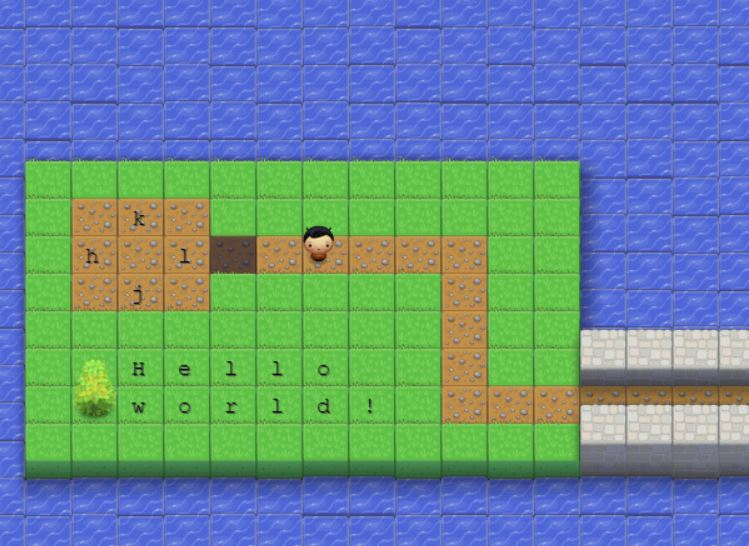
\includegraphics[width=0.6\textwidth]{vimadventures}
  \caption{\textit{Vim Adventures} Game Scene}
  \label{fig:vim-adventures}
\end{figure}

The value as a teaching tool lies inside the navigation commands for the player character. The controls for said navigation exactly match the navigation commands within the \textit{Vim} editor. While the player learns these commands (e.g., h,j,k,l keys for directional navigation as also shown in Figure \ref{fig:vim-adventures}) for in-game navigation these commands can simultaneously be used in the text editor. This allows for playful familiarization, possibly motivating the player/user to keep learning despite the steep learning curve of the editor itself. In conclusion this example shows how a carefully crafted game can be able to provide educational value in a non-gaming context. Thus, this approach could act as a blueprint for a possible implementation of a technology-aided onboarding solution.

Another approach was taken by \textit{CodinGame} \footnote{\url{https://www.codingame.com/}, accessed on 14th of August, 2021}. \textit{CodinGame} is a mixture between an \gls{ide} and a game and aims to educate developers on different programming languages and programming concepts. Within the \textit{CodinGame} environment, there are different tasks given to the player. These revolve around the visualization of the player character, game objects and enemies on a part of the screen, as can be seen in \textit{Figure \ref{fig:codingame}}.

\begin{figure}[h]
  \centering
  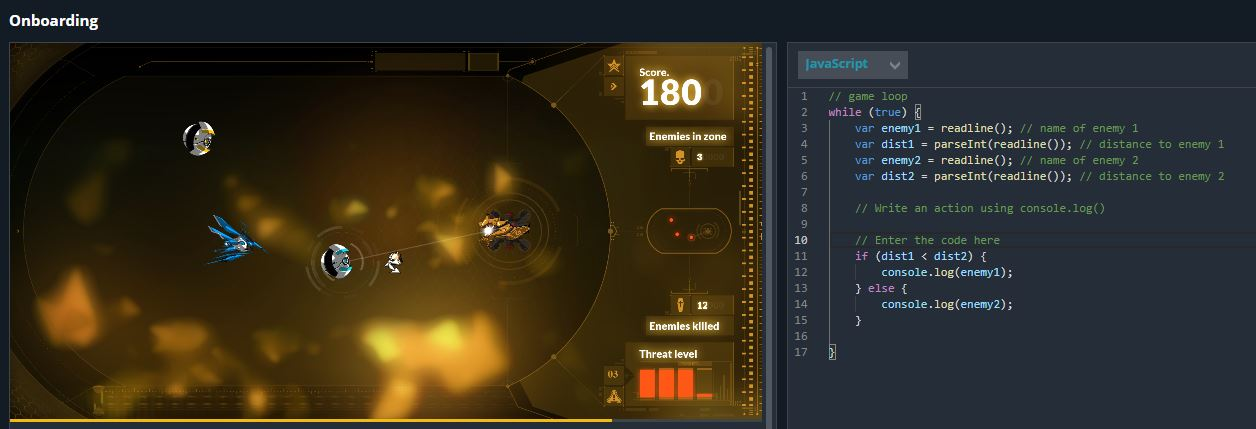
\includegraphics[width=0.9\textwidth]{codingame}
  \caption{\textit{CodinGame} Game Scene}
  \label{fig:codingame}
\end{figure}

Players then can tackle these tasks by writing valid source code in popular programming languages such as Javascript, C\#, C++, Java and more. Within the source code it is possible to reference the game objects entering the visualization on the other part of the screen. Through writing game-specific code you then are able to interact with these game objects to kill the enemy objects for example. After the player has written the necessary code, it is possible to re-run the respective game scene and thus see if the task has been successfully completed. Contrary to the previous example, \textit{CodinGame} does not try to teach concepts by matching mechanics to an outside concept. It rather uses writing source code as the central concept and only visualizes software development tasks playfully.

The \textit{Starbase} Game \footnote{\url{https://starbasegame.com/}, accessed on 14th of August 2021} represents another possible approach. Starbase is a massive multiplayer space adventure game. Unique to it, is its very detailed and intricate universe with a lot of different game mechanics and components to interact with. Instead of putting software development at the center or matching game mechanics to tool commands, \textit{Starbase} leverages software development in another way. Programming is used here as one of many game mechanics throughout the game. It allows for sophisticated control of in-game electrical devices. Code can be written in a custom programming language created specifically for the game. With that language nearly every technological device within the game universe can be controlled. To summarize, programming or learning commands connected to programming is not a goal in itself in this case. Instead, it is used just as a single mechanic within a game, where it allows for extremely fine-grained control over in-game components, which could be hard to implement visually.

Besides these sample applications of play from the industry there are also similar attem  pts irese One of them very recently by Lopez et al., where the usage of LEGO\textregistered Serious Play as an education tool for software development workflows was investigated \cite{lopez2021lego}. The study was setup in a way that students got handed a process definition to follow that matched popular project management techniques in software development. (e.g., a waterfall-style process and an agile process). Students then had to adhere to these processes with the overall goal to create a chair built out of LEGO\textregistered bricks. Depending on the given project management technique the process consisted of requirements, analysis, implementation, design, and evaluation phases in different orders. After students went through these phases, lecturers gave more context on these techniques and explained common pitfalls and advantages. Lopez et al. reported positive results within this study with students largely agreeing that it was highly fun and motivating to go through such processes playfully. The team environment together with lecturers acting as customers, allowed the students to hone their soft skills as well, as they reported. While this study does not resemble a game, it shows how toys can be appropriated into non-play contexts. This in turn allows for a playful learning experience, possibly increasing learning success.

Overall it can be said, that there is a great number of different approaches to utilizing the power of play in software development (or vice-versa, as shown with \textit{Starbase}) with different benefits gained from it. Within the implementation phase of the study, these different approaches could serve as possible implementation options. In essence these options are:

\begin{itemize}
  \item{Leveraging commands or tools used in software development as key game mechanics -- similar to \textit{Vim Adventures}}
  \item{Using source code created by the player as the main way of interaction within a game -- similar to \textit{CodinGame}}
  \item{Using programming as one of many mechanics in a game -- similar to \textit{Starbase}}
  \item{Using toys or other elements of play to visualize or simulate non-gaming concepts -- similar to Lopez et al.'s approach}
\end{itemize}

Concerning specifically using elements of play in the onboarding process of software development there is a clear lack of research, though. This reinforces the need for exploratory work into this exact topic, which ultimately is the goal of this thesis.

Lastly, after presenting these different approaches, there is one additional aspect of the software development context to clarify. The general openness towards integrating playful elements in such a process. A generalizable answer is hard to give in this case, given the large number of individual software developers already mentioned in this thesis' introduction. An attempt at answering the question can be made by investigating playful events and elements within the software development field. This could allow for an insight into the openness towards play.

One kind of those events are so-called \gls{ctf} contests. These have their origins in cybersecurity conventions. An example of such a contest would be the DefCon CTF\footnote{\url{https://defcon.org/html/links/dc-ctf.html}, accessed on 14th of August 2018}. Within such contests, teams of developers compete against each other by trying to compromise the other team's server. More specifically, teams are required \enquote{to leverage their knowledge of vulnerability detection} \cite[p. 134]{childers2010organizing} in order to attack and defend a virtualized host server. Points were then rewarded for both securing a team's own services but also compromising the enemy team's services \cite[p. 132-135]{childers2010organizing}. The competition as well as the special rule sets teams agree own definitely resemble elements of play that were already mentioned.

Another kind of event rising in popularity are so-called \textit{Hackathons}. These can be defined as:

\begin{quote}
  \textit{an event in which computer programmers and others involved in software development collaborate intensively over a short period of time on software projects [...]. These hackathons are encouraging of experimentation and creativity. and can be challenge orientated}

  \footnotesize{Gerard Briscoe, \cite[p. 1]{briscoe2014digital}}
\end{quote}

Briscoe also proposes that elements of the hackathons originated from so called \gls{lan} parties. These are gatherings \enquote{of people with computers or compatible computer game consoles} \cite[p. 3]{briscoe2014digital}. Therein one can see the playful origins of such events very clearly. But also the hackathons themselves show similar elements of play to the \gls{ctf} contests mentioned before with rule sets for the teams as well as possible competition. This holds true even more, when looking at \textit{game jams}. These can be defined as \enquote{an accelerated opportunistic game creation event where a game is created in a relatively short timeframe} \cite{kultima2015defining}.

Besides those events, there even are signs of playfulness within the daily work of developers. While the coding work itself normally revolves around rather strict programming structures and syntaxes, playful elements can be discovered there as well. Uncovering all of those is out of scope for this thesis, so one exemplary element is going to be presented here. As a short preface it has to be understood how software developers collaborate on source code. Typically, this is done with a version control system, where multiple developers are able to contribute code to. This is done by aggregating changes in source code, then attaching a message and ultimately pushing the code changes to a place where other developers can access these changes and build upon. The act of aggregating and attaching a message, is called \textit{committing}. This is a central command within version control systems, as the attached messages communicate meta-information on the code changes to team members. This communication is usually held rather short and precise, but even within these commit messages playful elements can be situated. An example for this is \textit{Gitmoji}\footnote{\url{https://gitmoji.dev}, accessed on 15th of August 2018}, a project that aims to include emojis within those commit messages. That usage of emojis, as Hjorth et al. point out:

\begin{quote}
  \textit{has been defined as playful (Sicart 2014 [original citation \cite{sicart2014play}]). This is epitomized by the playfulness of the paralinguistics -- emojis ('picture characters'), emoticons (typographic characters), stamps and stickers. [...] The use of paralinguistics has become an increasingly popular and playful way of personalizing digital media communications.}

  \footnotesize{Hjorth et al. \cite{hjorth2018beyond}}
\end{quote}

Overall one could assume that at software developers might be open towards playful elements given the field's occasional openness towards ludic features and events. These are not generalizable statements at this point, though. Therefore one of the additional goals of the upcoming study is to gather more data on this statement.

\subsection{Design Implications \& Attributes of Play}

After all the research done into possible theoretical foundations and related work in general, it is crucial to derive a set of attributes of play and possible design implications that inform the next chapters of this thesis. This is especially important for an informed study design and even more so for an informed implementation. Consequently, this is going to be done in the following. Based on the literature that was analyzed beforehand a non-exhaustive set of attributes are going to be derived. For each of these attributes, the theoretical grounding is presented as well. This is going to result in a list of attributes that inform playful design implications, that in turn serve as the foundation for further explorative research as is going to be laid out in chapter 3. The theoretical grounding mentioned, mainly is derived from Miguel Sicart's \textit{Play Matters}, as it extends upon much of what came before in research into play. It also contains numerous actionable implications to explore further upon -- in contrast to an also influential but more abstract and philsophical approach like Suits' grasshopper. Where applicable, implications and attributes from other contemporary works are also included.

The first attribute of play is, that \textbf{play is a balance between creation and destruction}. This is based upon on what Sicart describes as, \enquote{Play is the struggle between order and chaos, between the will to create and destroy} \cite[p. 5]{sicart2014play}. This statement can very well be transformed into an actual playful feature of an onboarding experience into a software development project. As such, it is a prime candidate to explore further in the study that is following.

\textbf{Utilize already existing ludic features of a context} is the next implication from literature, based on Rodriguez \cite{rodriguez2006playful}. Some of these ludic features were described in chapter 2.3 and can be built upon during the study.

Rodriguez also proposes to \enquote{embrace conceptual uncertainty as a generative source [...] begin designing frameworks for actions that may or may not be considered playful} \cite{rodriguez2006playful}. When transferring that to an actual design implication, this can be interpreted as \textbf{embrace uncertain outcomes of playful elements}. That arguably is less of a directly actionable implication, rather a consideration to make. Nonetheless it is a noteworthy addition to this list.

Another consideration Sicart mentions is that \enquote{Play not as an activity of consumption but as as an activity of production […] play is a way of engaging and expressing our being in the world } \cite[p. 5]{sicart2014play}, which means that \textbf{play is an activity of production}.

Next up is an implication taken from a case study Sicart presented in \textit{Play Matters}. There he describes the case of an application called \textit{The Accidental News Explorer}. It pulls random sources of news to show the user. Sicart describes it as a serendipitous approach, that \enquote{forces us to look at its choices with playful astonishment}. Thus, \textbf{utilize serendipitous events} can be included as a design implication.

Another crucial point brought up by Sicart is the idea of \enquote{disrupting the normal state of affairs by being playful [...] in that move, we reveal the inner workings of the context that we inhabit} \cite[p. 15]{sicart2014play}. This resonates extremely well with the overall goal of onboarding into software development projects. Within onboarding we want to reveal the inner workings of the project a developer is onboarded to, so there could be huge potential in applying Sicart's proposal to \textbf{disrupt the conventional state of affairs}.

One more implication with a lot of potential based on the context at hand, is described later on by Sicart, the idea that \enquote{creative appropriations of data reveal new knowledge through play [...] even in the most rigid of context} \cite[p. 28]{sicart2014play}. This points to playful visualizations of the context as a promising way to increase the context-specific knowledge. Therefore the respective design implication would be, to \textbf{visualize creative appropriations of data}.

An additional implication -- also presented as a case study by Sicart -- is derived from \textit{Newstweek}. \textit{Newstweek} is an application that alters news headlines of major providers in real time, \enquote{to playfully manipulate news consumption [...] shattering our assumptions on networks, news, and consumption of stories} \cite[p. 29]{sicart2014play}. \textbf{Playfully manipulate the normal state of affairs} is therefore a design implication that can be derived here.

Sicart continues to propose elements of playful designs specifically. He mentions them being \enquote{by definition ambiguous, self-effacing, and in need for a user who will complete them} \cite[p. 31]{sicart2014play}. This can be directly translated into an implication of: \textbf{Let the user complete intentionally ambiguous designs}. In the course of this argument Sicart also mentions that \enquote{what, playful design focuses on is the awareness of context as part of the design} \cite[p. 29]{sicart2014play}, so that is something to consider as well: \textbf{make the context a part of your playful design}. This also closely aligns to Bogost's statements on games as educational tools that are able to teach about certain concepts from a specific context.

\textbf{Create companions with personality}, is another design implication taken from Sicart's work. He specifically mentions this idea, while elaborating on Siri -- \enquote{Siri is a playful design that breaks our expectations and gives personality to software [...] Siri becomes a companion more than a tool} \cite[p. 32]{sicart2014play}.

Before tackling a larger subsection of implications, another noteworthy comment by Sicart is going to be considered. Within said comment, Sicart specifies that \enquote{playful designs could be described as somewhat successful toy designs, that is, as objects that by design allow users to toy around with them} \cite[p. 40]{sicart2014play}. Reconstructing that into a design implication makes for the statement of \textbf{think of designs as toys and let users freely play with them}.

Next up, the topic of \textit{procedurality} is mentioned numerous times by Sicart, who partly extends upon Bogost's work on procedural rhetoric. Therefore, multiple design implications can be inferred specifically on procedural designs. At first though, a short reminder on what those procedural systems are, they \enquote{generate behaviors based on rule-based models; they are machines capable of producing many outcomes, each conforming to the same overall guidelines} \cite[p. 4]{bogost2007persuasive}. In no particular order, these are the design implications derived for procedural systems as a whole and procedural toys specifically:

\begin{itemize}
  \item{\textbf{Allow the player to both watch the procedure unfold but also alter it} -- based on \enquote{procedural toys [...], are paradoxical objects that put their users in the double role of performer and voyeur [...] We play with them to see how they behave, how they react} \cite[p. 41]{sicart2014play}}
  \item{\textbf{Visualize the procedural world's conditions} -- based on \enquote{Procedural toys are mesmerizing because they are frames of the otherness, because they are tiny worlds that operate by their own condition} \cite[p. 43]{sicart2014play}}
  \item{\textbf{Let the player test the limits of the system} -- based on \enquote{Much of the joy in interacting with these procedural toys comes from testing their very propness as we figure out where the seams are and what we can build with them} \cite[p. 57]{sicart2014play}}
  \item{\textbf{Let the player explore and test without too much guidance} -- based on \enquote{Software toys like sim City and other procedural toys are also play spaces to a large extent -- spaces of possibility created to explore with rules in order to see what happens} \cite[p. 51]{sicart2014play}}
\end{itemize}

Moving on from procedural systems and toys, there are some more implications obtained from Sicart's statements. A statement that stood out was, that \enquote{designing for play means creating a setting rather than a system, a stage rather than a world, a model rather than a puzzle. Whatever is created has to be open, flexible, and malleable} \cite[p. 90]{sicart2014play}. This also resonates with the statement, that \enquote{the game designer proposes and deploys an object into the world, letting it speak for itself and be spoken through} \cite[p. 90]{sicart2014play}. Recontructing that into an actual implication, would mean \textbf{treat the design as a deployable, flexible object rather than a polished piece}.

In addition to the design implications from literature on play, there were also some specific guidelines on onboarding experiences discovered through the extensive literature review. Similar to the play focused design implications these are laid out in a non-exhaustive list as follows:

\begin{itemize}
  \item{\textbf{Recommend specific (easy-to-achieve) tasks to beginners} -- based on \enquote{To promote early exploration, newcomers are often assigned small bug fixing tasks, chosen to introduce them to the code while minimising risks to the rest of the team; this is because maintenance is regarded as requiring less design knowlege than new feature development} (\cite{latoza2006maintaining} as cited in \cite[p. 36]{yates2014onboarding}) and \enquote{One way to make the path easier is to point newcomers to easy tasks} \cite[p. 8]{steinmacher2018let}}
  \item{\textbf{Recommend experienced mentors to newcomers} -- based on \enquote{experienced developers are key to understanding a project} \cite[p. 284]{dagenais2010moving} and \enquote{Identify mentors or experts} \cite[p. 9]{steinmacher2018let}}
  \item{\textbf{Visualize the micro and macro structure of projects} -- based on \enquote{ What about creating useful maps: micro and macro views that show the relationships between different landscape features and routes that can be taken} \cite[p. 284]{dagenais2010moving}}
  \item{\textbf{Document the code structure} as laid out by Steinmacher et al. \cite[p. 10]{steinmacher2018let}}
  \item{\textbf{Identify and dismiss outdated information} as laid out by Steinmacher et al. \cite[p. 10]{steinmacher2018let}}
\end{itemize}

That concludes the list of design implications derived from literature on both the context and research into play and playfulness. These implications can now be used as a foundation for the next step within this thesis. As such, they are going to serve as one of the anchor points for the explorative study design described in the following chapter.
% Methodology
\section{Methodology}

After laying out the existing research and deriving implications from it, the next step consists of extending these findings. To achieve that a scientific study is in order. How that study is going to be structured is subject of discussion within this chapter. In the following the research questions are going to be revisited as a starting point for that discussion. For each of the unanswered questions adequate scientific methods to answer them, have to be found. To determine these methods in this chapter, at first additional considerations are laid out. After that, the chosen methodological area(s) is (are) described in more detail. The reasoning and final selection of methods are presented subsequently. Finally, the data generated through the chosen methods has to be analyzed. The way in which this is done, is illustrated at the end of this chapter.

\subsection{Methodological Considerations}

To choose the right methods for the research questions at hand, additional considerations have to be taken into account. These considerations consist of the nature of the question (is it an exploratory question, do we want to measure effectiveness, \ldots) and the goal of these questions. The first research question \textbf{(RQ1)} is, \textit{How and which theories \& concepts from research on play can be used in the onboarding process of software development projects and how are developers experiencing them?}. As this is the main research question it is not going to be answered using a single method but rather through collectively answering the other questions and condensing the results.

The second research question \textbf{(RQ2)} is: \textit{Which playful themes could lend themselves well to evolve software development projects into a spaces of play?}. These strategies, patterns, systems and theories can also be described as implications for those spaces. The foundation for these design implications was discovered in chapter 2.4. That foundation is expanded upon in the following chapter, where from these implications in literature implications for a possible design are formulated. The question of which of the implications are effective in onboarding processes is out of scope for this thesis though, as the focus lies in exploring possible implications to start with. Nonetheless, initial, qualitative feedback on a subset of implications that could be implemented should be gathered.

For the third research question \textbf{(RQ3)} -- \textit{What are the technical, social and personal intricacies of an onboarding context in software development and how do they influence the onboarding experience?} -- much of the research was already done. Similar to RQ2, the intricacies of the process were described through researching related literature on exactly this topic. Additional qualitative data should be gathered to answer RQ2 within the upcoming study. It is not the goal, however, to develop generalizable statements about the process. The overall goal is an exploratory one and therefore possible participant feedback is only used for the argumentation of the qualitative results.

In contrast to RQ2 and RQ3 for the fourth research question \textbf{(RQ4)} -- \textit{How can the identified themes be applied in actual onboarding settings?}, as well as the fifth research question \textbf{(RQ5)} -- \textit{How do different kinds of software developers experience playful aspects within an onboarding context?} -- there is no existing body of work to rely on. Therefore the upcoming study should aim to provide an answer to those two questions in specific and gather additional data for the aspects mentioned concerning RQ2 and RQ3.

To discover adequate methods, first RQ4 has to be deconstructed to uncover what exactly should be researched. There are two parts of the question that help with this. Firstly, the notion of  \textit{applied} and secondly the phrase \textit{in actual onboarding settings}. Applied, strongly points to the practical creation of something that incorporates the implications identified before. A possible approach for this could be to pick a single implication, implement it and then extensively test it with study participants. This could allow for generalizable results for this specific approach, where one could produce reproducible results. While such an approach could deliver valuable insights, the downside is its narrow focus on one implementation detail. Another approach could be to implement and maybe even combine multiple implications in one design and gather data on the participants' subjective experience towards them -- which would be the goal of RQ5. The design process of such an approach could also provide data on possible applications for multiple implementations, which in turn allows for a broader answer to RQ4. The downside of researching multiple implementations at the same time is the possible blending of effects of multiple implications. This means that no definitive answer on the effectiveness of one specific implication can be given. On the other hand it allows for participant feedback on multiple design implications, based on which future research can be done on promising aspects.

As one can see here, there is no \enquote{silver bullet approach} here, rather there are considerations to make on which approach provides more of the desired results. For this thesis these are -- as already mentioned more than once before -- very much focused on taking a step into uncharted territory and explore different paths within that. Thus, exploratory, open-ended results generally what is aimed for here, which makes for an easier weighting of the arguments presented. This means in the following methods are considered, that are able to deliver on this and produce data on a multitude of possible implications.

The second part of RQ4 (\textit{actual onboarding settings}) narrows down options for methods further. As an important aspect of this thesis as a whole is the combination of play with the context -- the aforementioned \textit{actual onboarding settings} -- investigating design implications within this context is necessary. This shows the need for a method where the implementation of the design implications can be deployed in the context.

A methodological area that could provide this is \textit{\gls{rtd}}, where through a design (e.g., the implementation of the identified implications) research can be done. Important to note here, is the need for additional data to answer the explorative and personal aspects of RQ2 through to RQ5 as mentioned earlier. To identify if \gls{rtd} as a whole and its specific methods in particular can deliver that, a more detailed description is given in the subsequent chapters. The chosen methods are then laid out in particular, as well as the chosen analysis methods.

\subsection{Research through Design}

To gain a clear picture of what \gls{rtd} is, it is important to understand the differences between design and research as a whole. Fortunately, Stolterman describes these differences very well. Research, or more specifically scientific research, he explains, drives towards the existing and to universal knowledge. Specifically Stolterman mentions that, \enquote{The aim of science is to formulate universal knowledge that explains the complexities of reality on a level removed from specifics and particulars} \cite[p. 57]{stolterman2008nature}.

On the other hand, \enquote{design deals with the specific, intentional and non-existing} \cite[p. 59]{stolterman2008nature}. Certainly this kind of research has proven very useful to generate \enquote{knowledge about natural objects and phenomena} \cite[p. 3]{simon2019sciences}. Research on and with man-made \textit{artificial} objects asks for a different science, as Simon has argued even back in the late 1960s \cite{simon2019sciences}. Simon also further defined aspects of such a science of design, describing designers as everyone who \enquote{devises courses of action aimed at changing existing situations into preferred ones} \cite[p. 111]{simon2019sciences}. This notion of creating preferred futures generally prevailed. Coughlan et al. specifically mentioned designing prototypes as a way to create such futures and contrasts it to the traditional science approach:

\begin{quote}
  \textit{In its essence as a design synthesis tool, prototyping represents commitment to a new future. In contrast, prolonged analysis of existing or historical practices (implicit in many of the articles in this issue), even though undertaken with the goal of future change, inevitably feels rearward facing}

  \footnotesize{Coughlan et al. \cite[p. 132]{coughlan2007prototypes}}
\end{quote}

As already mentioned before, this aligns with the goal of thesis overall -- to branch out into the future, to create new ways of how to onboard software developers. In addition to that there is a need to research a multitude of applied implications. Overall, this points at a designerly approach being the right methodological choice here. Critics might argue that such an approach is missing rigor and reproducability. While especially the aspect of reproducability cannot be denied, it has to be said, that \enquote{Design research conducted according to strict scientific procedures can produce highly valuable knowledge} \cite[p. 60]{stolterman2008nature}. To actually create this valuable knowledge, a strict scientific procedure has to be chosen and applied. This is where \gls{rtd} comes into play. The term was first coined by Sir Christopher Frayling \cite{frayling1994research} and brought into the field of \gls{hci} by Zimmerman et al. \cite{zimmerman2007research}. They describe \gls{rtd} in \gls{hci} as a way to produce novel integrations of research into HCI to create something, that represents the preferred state of the world \cite[p. 493]{zimmerman2007research}. \gls{rtd} as a whole can be described more broadly as a way to conduct scholarly research with methods originating from design practice \cite{zimmerman2014research} \enquote{as a legitimate method of inquiry} \cite[p. 310]{zimmerman2010analysis}. Zimmerman et al. also reinforces the arguments on why \gls{rtd} would be an adequate methodology in the case of this thesis:

\begin{quote}
  \textit{RtD allows researchers to rely on designerly activities as a way of approaching messy situations with unclear or even conflicting agendas; situations that are not well suited to other methods of inquiry. Additionally, RtD forces researchers to focus on research of the future, instead of on the present or the past.}

  \footnotesize{Zimmerman et al. \cite[p. 310]{zimmerman2010analysis}}
\end{quote}

Zimmerman also proposes criteria for evaluating \gls{rtd} approaches, to ensure that as much scientific rigor as possible is applied to such approaches. The four criteria proposed are:

\begin{itemize}
  \item{\textbf{Process} -- \enquote{In documenting their contributions, interaction design researchers must provide enough detail that the process they employed can be reproduced. In addition, they must provide a rationale for their selection of the specific methods they employed} \cite[p. 499]{zimmerman2007research}}
  \item{\textbf{Invention} -- \enquote{The [...] contribution must constitute a significant invention [...] researchers must demonstrate that they have produced a novel integration of various subject matters to address a specific situation} \cite[p. 499]{zimmerman2007research}}
  \item{\textbf{Relevance} -- \enquote{researchers must also articulate the preferred state their design attempts to achieve and provide support for why the community should consider this state to be preferred} \cite[p. 499-500]{zimmerman2007research}}
  \item{\textbf{Extensibility} -- \enquote{defined as the ability to build on the resulting outcomes of the interaction design research: either employing the process in a future design problem, or understanding and leveraging the knowledge created by the resulting artifacts} \cite[p. 500]{zimmerman2007research}}
\end{itemize}

Delivering on all those aspects is crucial in order to allow for valuable knowledge generation despite not following a traditional research approach. Therefore, these criteria are going to be referred back to throughout both the study and the results of this thesis, starting with the process. Creating such a process from scratch could weaken the study's results, as an unproven approach has to be validated in itself (independently from the results of its application). Thus, following and documenting a proven process as part of a proven set of methods is necessary here. Within \gls{rtd} a multitude of different methods emerged since its integration into \gls{hci}. Fortunately, Sanders condensed years of research on design research as a whole and condensed it into a map of said design research, as visible in \textit{Figure \ref{fig:researchtypes}}.

\begin{figure}[h]
  \centering
  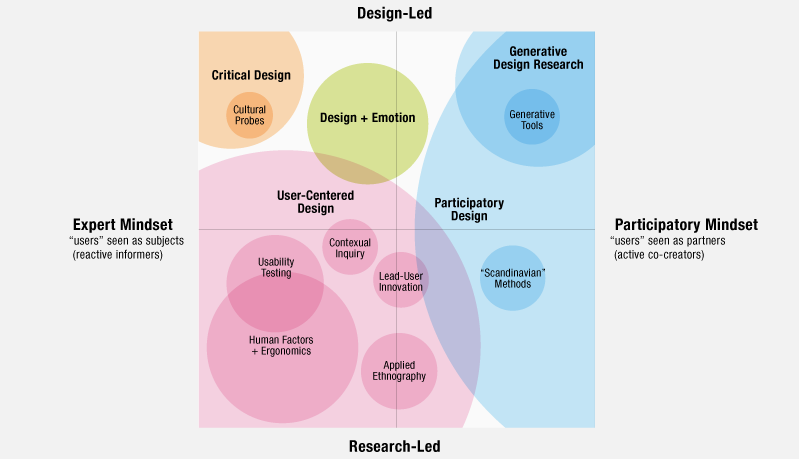
\includegraphics[width=0.9\textwidth]{researchtypes}
  \caption{\enquote{Map of design research -- research types} by Liz Sanders \cite[p. 3]{sanders2008evolving}}
  \label{fig:researchtypes}
\end{figure}

It is important to note here, that this does not show a map of \gls{rtd} methods specifically, but a more complete one of many methods applied in \gls{hci}. The two axis of the map describe firstly, which research type the methods align to -- either design-led or research-led, based on the distinction described earlier. Secondly the so-called \textit{mindset} focuses on if an expert creates something that then is relayed to the users or if the users are active co-creators as Sanders puts it \cite[p. 5-6]{sanders2008evolving}. \gls{rtd} can be located mainly in the upper-left quadrant of this map, although it can be argued that some methods include the user as a more active part. Generally, though, \gls{rtd} is based upon careful preparation by experts and therefore gravitates towards the aforementioned expert mindset. In \textit{Figure \ref{fig:researchtypes-probes}} Sanders extended her original map with some more methods.

\begin{figure}[h]
  \centering
  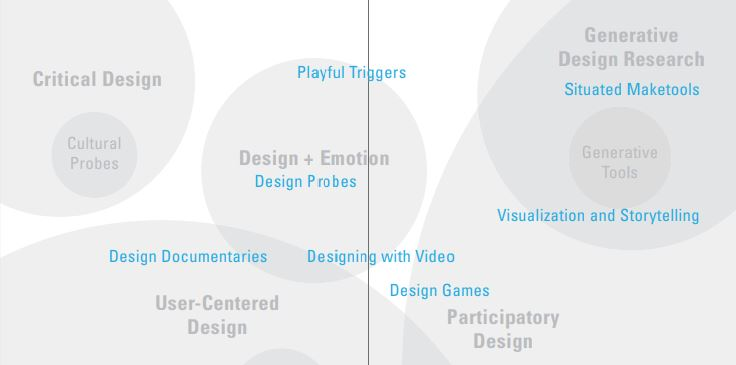
\includegraphics[width=0.7\textwidth]{researchtypes-probes}
  \caption{Upper section: \enquote{Map of design research -- new tools and methods} by Liz Sanders \cite[p. 6]{sanders2008evolving}}
  \label{fig:researchtypes-probes}
\end{figure}

To narrow down the methodological choices it is crucial to estimate where this study would fall within the presented map. Concerning the research-led vs. design-led, the case has already been made for a distinctly design-led approach. Regarding the mindset the answer is a bit less obvious. While we do want to gather information directly from developers in actual onboarding settings, this does not necessarily mean that they are participating in the design process itself. Most of the work on the theoretical foundation design is already done, therefore at that step, there is need for additional input. Where additional input \textit{is} needed, is at the transition from implemented implications towards recommendations and starting points for future research. An approach where both the expert mindset and partly active participation is possible, would thus be the desired one. On the map methods allowing for this would subsequently be located in the middle of the upper section.

In that section we can find the two methods \textit{Playful Triggers} and \textit{Design Probes}. The term \textit{playful} strongly suggests that this might be the right method to research play. Upon closer inspection it might not be fully applicable to this study, as \enquote{This methodology utilises playful, tactile, everyday qualities of objects} \cite[p. 16]{akama2010community} and then \enquote{take on the meanings placed on them by the participants} \cite[p. 16]{akama2010community} to facilitate conversation. This would align with the goal of researching how developers experience (and how open they are towards) such playful triggers in onboarding processes, but disregards the implementation part of the study. In addition to that tangible interaction together with facilitated on-site collaboration and conversation due to ongoing work-from-home mandates especially for software developers due to the COVID-19 pandemic. Therefore, it is required that the chosen method can be executed remotely. A closer look into \textit{Design Probes} consequently is the next step. As these exist in many variations, these have to be discussed in order to choose a suitable of these variations.

\subsection{Probing in a Digital Context}

Before delving into these variations, the origin of probing has to be mentioned, as it is going to help in understanding the process and goals of what came after. This origin can easily be traced back to Gaver et al., who first mentioned \textit{Cultural Probes} as a research method in 1999 \cite{gaver1999design}. Gaver et al. were tasked with researching novel interaction techniques for the elderly within their local communities. The difficulty they were faced with, was the cultural difference between them as the designers and experts and the elderly from different parts of europe. To overcome these difficulties, they developed these so-called cultural probes, \enquote{packages of maps, postcards, and other materials [...] designed to provoke inspirational responses from elderly people in diverse communities} \cite[p. 22]{gaver1999design}. According to Gaver et al. these probes \enquote{address a common dilemma in developing projects for unfamiliar groups} \cite[p. 22]{gaver1999design}. The aforementioned parts of the probes (postcards, maps and more) were designed to be approached casually and to spark open-ended discussion . The probes consisted of two other parts as well. Firstly, questions were included, that concerned the environment of the elderly. These were as open-ended as possible in order to give the participants as much room as possible to answer casually. Secondly the probes included a self-documenting aspect. Participants were tasked to take record specific actions daily for a week \cite[p. 22-26]{gaver1999design}. Concerning the particular goals, Gaver et al. also mention gaining \enquote{new understandings of technology} \cite[p. 25]{gaver1999design} and designing to \enquote{shift current perceptions of technology functionally, aesthetically, culturally, and even politically} \cite[p. 25]{gaver1999design}. Another important aspect is that the resulting data is not guided by any single objective problem statement, instead it is inspirational data that comes out of the process. The actual launch of the probes was then done in meetings at the local sites, after which the participants used the probes to self-document as described earlier. Finally, Gaver et al. also describe how, even though \enquote{the probes were central to our understanding of the sites, they didn’t directly lead to our designs} \cite[p. 29]{gaver1999design}. Cultural probes are widely used nowadays in \gls{hci} research \cite{crabtree2003designing,wyeth2006designing,kjeldskov2004using,celikoglu2017user,fisher2016adapting}. So widely used in fact that multiple variations developed from these cultural probes.

One that is particularly interesting in the context of researching digital artifacts are \textit{technology probes}. This term was coined by Hutchinson et al., who originally used it as a way to design technologies for and with families \cite{hutchinson2003technology}. They deployed two different technology probes in two different contexts, a \textit{VideoProbe} and a \textit{MessageProbe}. Independent from these different probes, what Hutchinson et al. wanted to achieve was to get knowledge and user feedback early on in the design process. Not only that, they wanted \enquote{them to be active partners in the design process} \cite[p. 2]{hutchinson2003technology}. Although it has to be noted, that Hutchinson et al. did not go so far as to \enquote{expect the family members to become designers} \cite[p. 18]{hutchinson2003technology}. It is also mentioned where exactly these \textit{technology probes} differ from \textit{cultural probes}, \enquote{cultural probes tend to involve a single activity at a particular time and do not stress technology per se} \cite[p. 18]{hutchinson2003technology}. The ultimate goal of a \textit{technology probe} is similar to that of traditional \textit{cultural probes}, albeit more focused on a specific technology: \enquote{Ideally, technology probes will spark new ideas and help the families articulate ideas for the prototypes we will build} \cite[p. 18]{hutchinson2003technology}. To create a \textit{technology probe} that can achieve such a goal, Hutchinson et al. define the five following features:

\begin{itemize}
  \item{\textbf{Functionality} -- \enquote{Technology probes should be as simple as possible, usually with a single main purpose and two or three easily accessible functions} \cite[p. 18]{hutchinson2003technology}}
  \item{\textbf{Usability} -- \enquote{Technology probes are not primarily about usability in the HCI sense, so during the use period, we do not change functions} \cite[p. 18]{hutchinson2003technology}}
  \item{\textbf{Logging} -- \enquote{Technology probes collect data about relationships within the family and help family members (and us) generate ideas for new technology} \cite[p. 18]{hutchinson2003technology}}
  \item{\textbf{Flexibility} -- \enquote{technology probes [...] should be designed to be open-ended with respect to use} \cite[p. 19]{hutchinson2003technology}}
  \item{\textbf{Design Phase} -- \enquote{Technology probes are intended to be introduced early in the design process as a tool for challenging pre-existing ideas and influencing future design} \cite[p. 19]{hutchinson2003technology}}
\end{itemize}

These would be the criteria a possible technological implementation in the upcoming study strives for. This is in contrast to a prototype, that is much more feature rich from the beginning, focuses on usability and improved iteratively (rather than implementing something new based on the data gathered through a probe) \cite[p. 18-19]{hutchinson2003technology}. Generally speaking one could describe these technology probes as a kind of middle ground between, cultural probes with no preceding implementation, and the evaluation of full-blown prototypes. This is also in contrast to so-called \textit{digital cultural probes}, as e.g., Iversen \& Nielsen applied it \cite{iversen2003using}. They went for more of a traditional approach with a stark focus on self-documentation and content generated by the participants, rather than deploying an implementation for them to use.

At this point, the questions arises on what to take from all of that regarding the methodological decision at hand. Answering that question requires contrasting the goals of our research with what probes in general and \textit{technology probes} in particular provide. The overall goal of the thesis is to explore new opportunities for playful approaches in an onboarding context as mentioned numerous times before. Thus, there is a need for a method that at its core is exploratory. Probes  certainly can provide that, as Mattelmäki describes in her doctoral thesis on \textit{Design Probes} as whole. She writes, that \enquote{probes have an exploratory character. They explore new opportunities rather than solve problems that are known already} \cite[p. 40]{mattelmaki2006design}. Another important point mentioned mainly in RQ5 is the need to research how software developers specifically experience playful aspects. Researching this could arguably be the biggest strength of probing. Mattelmäki describes it as follows, \enquote{probes look at the user’s personal context and perceptions. The purpose is to outline human phenomena and users, as well as introduce the user’s perspective to enrich design} \cite[p. 40]{mattelmaki2006design}. This is also described by Gaver et al. as \enquote{The real strength of the method was that we had designed and produced the materials specifically for this project, for those people, and for their environments} \cite[p. 29]{gaver1999design}. \textit{Technology probes} in particular can provide even more value in the case of this thesis. RQ4 and RQ5 also call for testing out implementations of the design implications in real-world settings, while still being open towards new input from developers. Referring back to Hutchinson et al., they describe the goals of \textit{technology probes} as:

\begin{quote}
  \textit{the social science goal of collecting data about the use of the technology in a real-world setting, the engineering goal of field-testing the technology, and the design goal of inspiring users and designers to think about new technologies}

  \footnotesize{Hutchinson et al. \cite[p. 17]{hutchinson2003technology}}
\end{quote}

This, again, closely aligns with the research goals of this thesis -- there is the need for collecting data about the design implications in \textit{actual onboarding settings}. There is also the need to \textit{field-test} these digitally implemented implications. Finally, there is also -- as mentioned before -- the need to still be open about new input, enriching what was discovered in literature. Overall, the clearly visible alignment of goals point towards \textit{technology probes} as a method of choice for the study. The relatively good adoption of this method (e.g. in \cite{fitton2004probing,o2006holding,edwards2011exploring}) further manifests it as an adequate choice.

Now, the only thing left is to define a rough overall process for the execution of this method. That process is then elaborated on in great detail in chapter 4 to ensure the study manages to meet the quality criteria for a well done \gls{rtd} approach, as described by Zimmerman \cite[p. 499]{zimmerman2007research}. It is crucial to mention some environmental constraints to the study here. Firstly, we are working with digital source code with which the participants (software developers) have to (mostly) interact with in a digital environment. Secondly, as acknowledged before, as of June 2021, there are many software developers choosing or being ordered to work from home due to the COVID-19 pandemic. Therefore, it is necessary that the chosen process can be done fully remotely.

There is no single process to follow when designing, executing and analyzing \textit{probes}. Gaver et al. even mentioned, that the \enquote{probes were not designed to be analyzed, nor did we summarize what they revealed about the sites as an explicit stage in the process} \cite[p. 27]{gaver1999design}. Hutchinson et al. on the other hand mentioned \textit{logging} and analyzing these logs as a distinct part of the process, as described before. How this is done specifically differs from study to study. Edwards et al. for example, logged user-generated data and created accompanying questionnaires to collect quantitative data on the participants use of their probes \cite[p. 107-110]{edwards2011exploring}. Mattelmäki proposes personal interviews to \enquote{extend, supplement and revise the signals collected in the probes} \cite[p. 86]{mattelmaki2006design} where qualitative data is generated. Ultimately, there is great variance in the execution as well as the analysis of these probes, as such it is even more important to carefully lay out every part of the final process.

Overall, there are three distinct areas that are part of the process, the development \& implementation of the probes, the execution \& deployment of the probes and the analysis of the data generated through the probes. Concerning the development of the probes, the path is pretty clear, as the features within the probe should be based on the identified design implications. The specific process of how these were transformed into probe features is therefore described in great detail in chapter 4.2 and specifically in the sub-chapter 4.2.1. After the \textit{technology probe} with a set of features is developed it then has to be deployed into the context and executed by the participants. Therein it is important to gather the data needed to answer the research questions. Generation of data on personal experiences, as well as exploratory data is paramount.This strongly suggests collecting qualitative data, as it is uniquely able to gather perspectives of participants \cite[p. 7-8]{flick2018introduction} as well as generating new knowledge on a setting too pluralized for quantitative approaches \cite[p. 4-5]{flick2018introduction}. That does not mean there is no structured data at all, though. As \textit{logging} is such an integral part of \textit{technology probes}, user interaction with the features of the probe is going to be logged accordingly. To get an even more complete understanding of how the individual participants experienced the probe and to gather qualitative input on new ideas from participants, qualitative questions are going to be asked after probe execution. Additionally, to get a sense of how effective the probe features were in actually transmitting information about a project, questions on the project at hand are asked as well. This allows for a rich set of data for each participant to analyze. The focus strongly lies on generating as much valuable data as possible for each participant rather than aiming for a maximum number of participants. Overall there is going to be a three-step process concerning the probes:

\begin{enumerate}
  \item{Probe Development}
  \item{Probe Execution \& Data Collection}
  \item{Probe Analysis}
\end{enumerate}

As mentioned, the specific tasks within these steps are going to be described in great detail with every additional process choice documented as well in chapter 4. Concerning the probe analysis, the methods of analyzing the generated data is subject of the following chapter.

\subsection{Data Analysis}

The last high-level methodological choice to make is concerned with how to analyze the data gathered by the probing. To recapitulate, data is going to be gathered through these four methods:

\begin{itemize}
  \item{\textbf{Demographic Information} -- Prior to the probes some information on the professional background of the participants is gathered to gain a comprehensive picture of the participants}
  \item{\textbf{Participant Interactions} -- Throughout the probe the actions taken by the participants are going to be logged and categorized in an automated way (e.g. a click on an element on the screen)}
  \item{\textbf{Questions on the underlying project} -- The participants are going to be asked questions on the project they are onboarded on to}
  \item{\textbf{Questions on the research topic} -- The participants are going to be asked questions centered around the research topic to gather their expertise and ideas on the topic}
\end{itemize}

In order to correctly analyze that data, it is crucial to know what kind of data is generated by each of these. Only after that a suitable method of analysis can be found. Starting with the demographic information, which can easily be identified as fixed data types (e.g., age always equals a number). These do not have to be analyzed on their own, they rather set the data in an individual context for each of the participants. The interactions on the other hand are going to be automatically logged during the study. Therefore, the logs need to follow a predefined structure in order to log a variety of different interactions. The actual structure of these interactions is described in chapter 4.3 as it also depends on the technology used to capture these events. The interactions could be analyzed in a way to find patterns of interactions, like analyzing the number of clicks at a certain point in time. This might be very useful to delve into specific aspects of the probe and analyze them in great detail (see Fitton et al. for example \cite{fitton2004probing}). While this can be useful for intricate features, these are not really the part of the probes, as it should be kept simple. In addition to that evaluating the effectiveness and details of these particular features is not the prime goal of this study. Nonetheless, it can help in solidifying arguments based on the other kinds of data and can be referred to together with the participants feedback. Because of that the interactions together with the time of that interaction is going to be logged but only analyzed in detail as needed depending on the other data. Simple aggregations of total interactions and total time spent within the probe are generated from the raw logs, though, to give a sense of how active the in-probe interaction was. Moving on to the questions on the underlying project, these as well should help in understanding how the participants experienced the probe. The goal of these questions should be to understand if some of the underlying information was transported successfully. The questions should be crafted in a way, that allows to verify if the participants recognized the project information. Lastly, the arguably most important part is to gather data on the experiences of the participants, their attitude towards playfulness in onboarding processes and their ideas on how to integrate it. As already described in the previous chapter a qualitative approach was chosen for that. Concerning the actual creation of the questions, these are centered around the specific topic at hand, similar to how problem-centered interviews are structured around an issue \cite{witzel2012problem}. The actual data collection for these problem-centered interviews revolve mainly around in-person enquiries, mirroring and lively discussion \cite[p. 232-236]{flick2018introduction}. Due to the study being a remote one, such a lively discussion might be at harder to execute. Therefore online interviewing, as mentioned by Flick \cite[p. 243]{flick2018introduction} could be a more adequate solution. This type of interviewing can be done in a few different ways. Probably, the two most important decisions concerning the study design are, if the questions should be answered asynchronously or synchronously, and through which medium the questions are asked. This largely depends on the study setup, as it could be possible to integrate the questions within the probe or the medium over which the probe is interacted with. Thus, the final decision rationale is described in the subsequent chapter. This final decision does not change the method to analyze the data, as this data is unstructured text that is going to be used for qualitative argumentation. Depending on the amount of data gathered there are different options for the following analysis. From using the participant directly to support argumentation to applying a specific method of analysis, there is a broad range of possibilities. On the more rigorous end of the scale, two of the most notable approaches are thematical analysis \cite{braun2006using} and content analysis \cite{schreier2012qualitative}. These mainly differ in their starting point, where themes are generated from text (thematical analysis) or a text is analyzed with a set of categories in mind (content analysis) \cite[p. 490]{flick2018introduction}. Concerning the research done within this thesis, a lot of themes and implications were already discovered, therefore it might make a lot of sense to use them as a starting point for the analysis. This should make content analysis a suitable choice for analyzing the data. Executing such a content analysis procedure involves multiple steps, as described by Schreier and Flick (\cite[p. 174]{schreier2014ways}, \cite[p. 483-485]{flick2018introduction}:

\begin{enumerate}
  \item{Selection of the material}
  \item{Creation of a category system}
  \item{Segmentation of the material}
  \item{Main coding}
  \item{Interpretation and Presentation}
\end{enumerate}

Within those steps, additional methodological decisions and considerations have to be made. Concerning the first step, the respective selection is an easy one to make. As the study is specifically crafted in order to generate qualitative data, all the qualitative answers within that study are subject to the analysis. Thus, all answers by each participant on the research topicnd on the underlying project are selected for the content analysis. The additional data collected throughout the probing is used as a support for the result argumentation, as was mentioned before.

Regarding step two, the creation of a category scheme, there are three distinct options of coming up with these categories: \textit{Deductive, Inductive and Deductive-Inductive}. The decision on one of these approaches mainly depend on if the result argumentation should be derived from the material (inductive) or defined by literature and brought to the material (deductive). Mixed approaches exist as well, where some categories are brought to the material and some are based on the material (deductive-inductive), by defining top-level categories from literature and lower-level categories from literature for example \cite{schreier2014ways}.

This is what is going to be done in the case of this study, with the overall direction of the analysis defined through the literature and the research questions, while also allowing for new categories and themes based on text.

Concerning step three, a unit of segmentation has to be defined. Two options -- that can again be mixed and inform each other -- are coding units and contextual units. Coding units carry meaning by themselves and can be definitively allocated to a category, while contextual units only help in giving meaning to the coding units \cite{schreier2014ways}.

In the context of this study, the material is divided into coding units. Where necessary or helpful to give context, contextual units are used. These contextual units can either be the features/questions they refer to, but also the logged data, where it supports the argumentation.

The coding itself is then done as a two-step process, with marking important units at first and then coding these marked units in a second step, as described by Schreier \cite{schreier2014ways}.

The interpretation and presentation ultimately can be found in detail in chapter 5.2 onwards.
% Research Design (& Probes ?)
\section{Research Design}

After laying out the methodology used throughout the study, the actual application of the methodology has to be described. In the following chapter, considerations on research ethics, as well as participant selection are discussed. In addition to that, the development of the technology probes, the process for going through these probes, the technological setup for data collection, and the data analysis approach are documented in detail. The study approach as a whole is then summarized at the end of this chapter.

\subsection{Research Ethics}

Before delving into the specifics of the study an important, sometimes neglected, aspect of the study design has to be talked about: \textit{Research Ethics}. In order to execute an ethically sound study with participants, some important principles have to be met. Flick proposed eight principles of ethical research, that this study aims to follow (taken from Flick \cite[p. 135]{flick2018introduction}):

\small{
  \begin{enumerate}
    \item{\textit{Researchers have to be able to justify why research about their issue is necessary at all}}
    \item{\textit{Researchers must be able to explain what the aim of their research is and under which circumstances subjects participate in it}}
    \item{\textit{Researchers must be able to explicate the methodological procedures in their projects}}
    \item{\textit{Researchers must be able to estimate whether their research acts will have ethically relevant positive and negative consequences for the participants}}
    \item{\textit{The researchers must assess the possible violations and damages arising from doing their project}}
    \item{\textit{The researchers have to take steps to prevent violations and damages identified according to principle 5 above}}
    \item{\textit{The researchers must not make false statements about the usefulness of their research}}
    \item{\textit{The researchers have to respect the current regulations of data protection}}
  \end{enumerate}
}

To meet these requirements towards ethics, participants have to be informed on each of the principles mentioned above. To achieve this, both a form of consent and a data protection information sheet have been created, which can be found in appendix \ref{append:consent}. Principles 1 through 3 should be met, by describing in the beginning paragraph and the subsections \textit{General Study Information} and \textit{Overall Study Procedure} of this form. Concerning principles 4 through 6, there should not be any positive or negative consequences for the participants, as the study only consists of a virtual probe with questions on the expertise of the participants, not on personal or intimate details. Should the participants wish to participate anonymously, an option to do so is given as well. If the participants check this option in the online form, the gathered data is stored by using a random identifier number not connected to their name. As for principle 7, no false statements on the goals of the research are made, the goals match those mentioned within this thesis.

Finally, the last principle is met by including all relevant information on the specifics of data processing in the subsection \textit{Confidentiality and Data Processing}. Therein everything that is logged is described together with where and how it is logged and processed. To make it clear for participants that withdrawal of participation is possible at all times, an additional section (\textit{Rights}) is added to the form. The resulting form is then presented to every participant before they start taking part in the probe and without consenting to it the probe cannot be started.

In addition to the considerations that are part of the consent, due to the current, ongoing COVID-19 pandemic, there are additional considerations to be made. These mainly revolve around not requiring the participants to take part in a study on-site. As mentioned before, the probe is going to be done remotely, therefore, there is no need for additional precautions have to be taken on that account.

\subsection{From Theory to Probe}

The most important part of the research design arguably is the technology probe. As described in the methodology section, this requires careful attention to the features described by Hutchinson et al -- \textit{Functionality, Usability, Logging, Flexibility, Design Phase} \cite[p. 499-500]{hutchinson2003technology}.

The functionality is determined by the design implications found in literature and described in detail in the following chapter. Concerning the usability, Hutchinson et al. only state that there should not be any incremental changes during a probe, therefore this is not further elaborated on. Logging is going to be part of the data collection phase of the probe and therefore is described in the respective chapter. Finally, concerning the design phase, the probe is developed as the very start of the design process within this thesis.

A crucial part of developing the technology probe is the transition from theory to a finished probe to the execution of that probe. Therefore, this chapter is mainly concerned with the tasks done and decisions made in between those steps. At the start of this process is the transformation from the design implications and attributes of play  into actionable probe features. This again is divided into multiple sub-steps, the first of those steps being an ideation phase. Within that ideation phase, the design implications are used as a starting point based on which possible features, playful elements, and game mechanics are ideated upon. This is loosely based upon IDEO's brainstorming principles \cite{ideo2021brainstorming}, as can be seen in \textit{Figure \ref{fig:probeideation}}.

\begin{figure}[h]
  \centering
  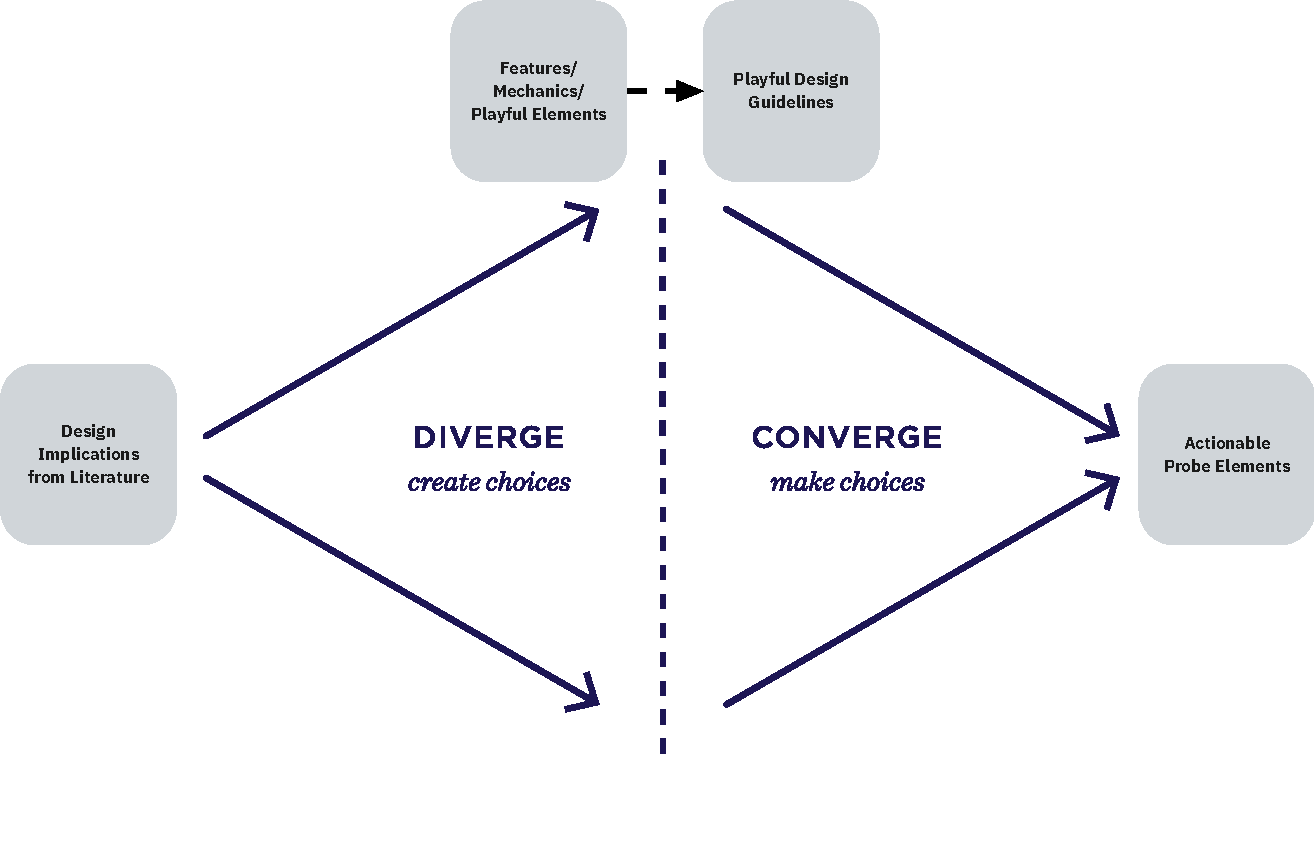
\includegraphics[width=\textwidth]{probeideation.pdf}
  \caption{Adapted IDEO Brainstorming Process (originally by IDEO U \cite{ideo2021brainstorming})}
  \label{fig:probeideation}
\end{figure}

Starting with the design implications as many features/concepts/playful elements as possible are ideated upon to generate a variety of technological choices rooted in literature. With those generated, the next step is to \textit{make choices}, which means deciding on a few that then can be implemented as part the technology probe. Concerning this thesis, the respective brainstorming process is visualized and documented in \textit{Appendix \ref{append:probe-design}}. Therein you can see the implications on the far left of the diagram, based on which a braindumping session \cite{ia2021dumping} was held. The result of this session is visualized to the right of the attributes of play within \textit{Appendix \ref{append:probe-design}}. Examples of the ideas gathered are:

\begin{itemize}
  \item{Serendipitous random effects within the game/probe}
  \item{Generate game objects for contributions and possible tasks}
  \item{A Stage where the players can explore for themselves}
\end{itemize}

For the full list, refer to the respective diagram in the appendix. What is also shown in this diagram, is what kind of design implication the respective idea is based upon. These ideas were then condensed into actual guidelines that can inform the probe implementation or any kind of playful design for that matter. After that, converging these guidelines is necessary. This is done for two reasons. One, to reduce the number of features in order to conform to the technology probe attribute of \textit{functionality} described by Hutchinson et al. \cite[p. 18]{hutchinson2003technology}. Two, in order to create actionable tasks to inform feature implementation. The results of this process can be seen in detail in \textit{Appendix \ref{append:probe-design}}. The converging itself was done by combining and reducing the guidelines so that an implementable task description is reached. If some guidelines were not included as features, these were dismissed by me based on the perceived difficulty of implementation. That is because the technology probe should be kept simple and focused on gathering as much valuable data as possible rather than being an intricate and detailed prototype implementation.

Another important decision to be made at this point is which onboarding level the probe should focus on. Should it be on the source code/programmatic level, should it be at the process level or should it be at a social \& developer-centered level. This decision depends on a few things. At first, it has to work in a remote, decentralized setting due to the constraints defined in the previous chapter. Secondly, it has to be \enquote*{implementable} by me, based on the timeframe and my previous experience. Thirdly, and arguably most importantly, the probe should be able to collect data, that contributes to and extends the line of research. Concerning this third statement, there is no actual constraint imposed by existing research, as on none of the described onboarding levels, there are existing playful implementations in research. The first and second statement on the other hand do impose some constraints.

Because of the remote setting, a social setting might be hard to replicate remotely. In addition to that, as is going to be described in chapter 4.5, the study is not going to be done within one single team of developers working on one project, rather the probe is targeted towards individual developers. This further increases the difficulty in deploying a probe within a social setting. Therefore the probe is rather going to focus on program comprehension and process-centered techniques like information seeking and feature location, which can be implemented on a source code/project level. Nonetheless, research into the other levels of onboarding could be equally valuable in the future.

At this point, most of the non-technical decisions have been made. An ideation phase, followed by a phase of converging of those ideas, produced a set of possible features that can be implemented. As mentioned before, these are shown in the second-to-last column in \textit{Appendix \ref{append:probe-design}}. Actually deciding on the feature set used in the probe, depends on some technical decisions, though. This is why in the following chapter there is going to be a deep dive into all technical considerations including the final feature set.

\subsection{Probe Implementation}

To implement a coherent technology probe, these considerations have to be discussed in detail, starting with the choice of technology with which to implement the probe. As described in the previous chapter, the probe is going to target the psychology- and process-centered level of onboarding and is based on the source code and meta-information of a project. Best-case this probe could be applied to any project independently from its technology. Depending on the programming language and framework there are grave differences in project structure, though. A \textit{Ruby on Rails} \footnote{\url{https://rubyonrails.org/}, accessed on 10th of August 2021} project for example, gives the developer a fixed structure out of the box, while there is no such structure when developing a \textit{node.js} \footnote{\url{https://nodejs.org/en/}, accessed on 11th of August 2021}, project with \textit{express.js} \footnote{\url{https://expressjs.com/}, accessed on 11th of August 2021}. Creating a probe that would work with both of those examples or even more than that, would not be feasible in the given timeframe. More importantly, for a probe meant to be executed once by each participant, there is no benefit in investing additional implementation time into allowing the probe to work on multiple, differently structured projects in succession. In the case of this probe, the underlying project is not going to be changed for each participant to achieve some amount of comparability between the experiences of the developers. Deciding on which specific project and technology to choose depends on some constraints as well, though.

First of all, for a probe that can be sent out to developers not necessarily working within the same company and/or team, the source code of the underlying project has to be publicly accessible. This rules out projects proprietary to a single company right away. In addition to that, the project should cater to the knowledge of a wide variety of developers. Therefore, the technology used within the project underlying the probe should be popular enough, that a general understanding of the project setup is possible for the participants. According to a survey done by StackOverflow Insights \footnote{\url{https://insights.stackoverflow.com/}, accessed on 11th of August 2021} with 83,052 responses on the topic of programming languages developers have done extensive development in the last year, there is a clear leader in popularity (multiple responses by developers were possible): \textit{Javascript} (64.96\% agreement), its server-side framework \textit{node.js} (33.91\% agreement) and its superset \textit{Typescript} (30.19\% agreement), with the closes other technology/programming language being \textit{Python} (48.24\% agreement) \cite{so2021}. Thus, choosing a \textit{Javascript, node.js} or \textit{Typescript} project, might be the most approachable for a wide variety of developers. The only downside to choosing such a project is that none of these technologies by themselves give a fixed structure to rely on when building a probe upon it. Something that gives that structure, is the concept of monorepos.

These are repositories, where the \enquote{codebase is contained in a single repo encompassing multiple projects} \cite[p. 226]{jaspan2018advantages}. This gives inherent structure to the project, with different subprojects to explore. Also, larger codebases might profit more from onboarding help due to the increased complexity going hand in hand with the increase in size. Moreover, in a well-crafted monorepo, any \enquote{project in the repo can be built only from dependencies also checked into the repo} \cite[p. 226]{jaspan2018advantages}. This allows for visualizations of these connections within the monorepo and how subprojects relate to each other. Especially so, when combined with \textit{Javascript}-based monorepo-organization tools like \textit{Lerna} \footnote{\url{https://lerna.js.org/}, accessed on 11th of August}. \textit{Lerna} stores information on the dependencies within the monorepo in two files, \verb|package.json| and \verb|lerna.json|. In addition to that, the subprojects are guaranteed to be found in a \verb|/packages| directory. This further allows for reading these files and directories in code in order to easily implement probe features on top. Consequently, a \text{Javascript/Typescript}-based monorepo that uses \textit{Lerna} or a similar tool, with a predefined structure, where also the source code is publicly available has to be found. Fortunately, the largest provider of publicly available repositories, \textit{Github} \footnote{\url{https://github.com/}, accessed on 12th of August 2021} makes it possible to filter for these criteria (filter results can be found here \footnote{\url{https://github.com/topics/monorepo?l=typescript}, accessed on 12th of August 2021}). A highly popular monorepo, that is well maintained and actively collaborated on, is the \textit{ethereumjs-monorepo}, a repository containing the \textit{Javascript} implementation of the \textit{Ethereum} blockchain \footnote{\url{https://ethereum.org/en/}, accessed on 12th of August}. While this repository does not use \textit{Lerna}, it still follows the structure imposed by \textit{Lerna}, making it possible to programmatically read the monorepo information from its directories and \verb|package.json| file(s). Because of that and the repository matching the other constraints imposed on this decision, the \textit{ethereumjs} monorepo is chosen as the underlying project for the implementation of the technology probe.

The next decision to make is with which technology and in which in environment the technology probe should be created. Due to the setting as a remote probe, the technology used for the probe should be easy to distribute to the participants without any additional setup work on the researcher's, but also the participant's side. The perhaps easiest way to achieve this is to create an interactive web page, accessible through just a browser without any additional installation steps required. The downside of this approach would be, that the probe is removed from how most developers interact with the source code of a project -- through an \gls{ide}, text editor, or the command line. Due to a multitude of editors and \gls{ide}s existing, a decision on one of those tools would be necessary. This in turn limits the number of developers being able to take part in such a probe. In addition to that different editors and \gls{ide}s use different plugin systems, for which a non-negligible amount of previous experience is required to develop plugins in. This, together with my extensive experience in a web environment and with web technologies led to the decision of implementing the probe in such an environment.

Based on these decisions, the final feature set can ultimately be defined. Referring back to Hutchinson et al.'s probe features, a further reduction of features is in order. Therefore, special attention is paid to decide on a set of playful features, that can be transformed into a coherent probe. What also went into consideration, was an attempt to match probe features with concepts from the underlying project, to foster it being used as an educational tool -- similar to how Ian Bogost defined them \cite{bogost2007persuasive}. This led to the implementation of the following features:

\begin{itemize}
  \item{\textbf{Visualizing the overall project structure} -- Based on the idea that the code structure should be documented \cite[p. 10]{steinmacher2018let} and that the micro and macro structure of projects should be visualized \cite[p. 284]{dagenais2010moving}, as well as Sicart's notion of visualizing creative appropriations of data \cite[p. 28]{sicart2014play}}
  \item{\textbf{Free exploration within subprojects} -- Based on the idea that playful objects should be freely interacted with (based on Sicart's notion in \textit{Play Matters} \cite[p. 40]{sicart2014play}) and the idea that players should explore and test without too much guidance (based on Sicart's notion in \textit{Play Matters} \cite[p. 57]{sicart2014play})}
  \item{\textbf{Implementation of a reveal mechanic to uncover objects in subprojects} -- Based on the idea that users should complete intentionally ambigious designs (based on Sicart's notion in \textit{Play Matters} \cite[p. 31]{sicart2014play}) and the idea that uncertain outcomes should be embraced, where the user can decide (based on Rodriguez as described in chapter 2.4 \cite{rodriguez2006playful})}
  \item{\textbf{Discovery of potential issues} -- Based on the idea, that specific tasks should be recommended to the newcomers in a project (based on \cite{latoza2006maintaining}, \cite[p. 36]{yates2014onboarding}, and \cite[p. 8]{steinmacher2018let})}
  \item{\textbf{Discovery of important contributors} -- Based on the idea, that social links in development projects are crucial and mentors should be recommended to newcomers (based on \cite[p. 8]{steinmacher2018let} and \cite[p. 284]{dagenais2010moving})}
  \item{\textbf{Discovery of 3rd-party packages used} -- Also based on the idea of visualizing the micro and macro structure of a project \cite[p. 284]{dagenais2010moving}, where 3rd-party packages are part of both the code (=micro) and the overall structure (=macro) depending on the package}
  \item{\textbf{Creation of a companion helper} -- Based on the idea, that a companion with personality enables playfulness (based on Sicart's notion in \textit{Play Matters} \cite[p. 32]{sicart2014play}}
\end{itemize}

These features can be combined into a coherent \textit{game world}, that visualizes the project structure but also enables the players to playfully explore specific parts of the project. While the companion feature deviates from this coherent set, it nonetheless can be implemented as a tool of communication and occasional helper for the other features. Overall this should allow the technology probe to be succinct enough in functionality (again referring to Hutchinson et al. \cite[p. 18]{hutchinson2003technology}) while also being open-ended (as mentioned by Hutchinson et al. as well \cite[p. 19]{hutchinson2003technology}) enough in paths towards the exploration.

With that decided upon, the actual implementation now can commence. This implementation can be split into two distinct parts. Firstly, the generation of the \textit{game world}, and the discoverable elements of the probe from the underlying project. Secondly, the actual implementation of the user-facing, interactive part. These are described in detail as follows, starting with the user-facing implementation as the generation of the game world is based on how it should be visualized in the end.

\subsubsection{The User-Facing Implementation}

First of all a general idea of how the probe should be visualized aesthetically. Aesthetics play a vital role in the creation of any kind of probe. Gaver et al. point out, that they \enquote{believe aesthetics to be an integral part of functionality} \cite[p. 25]{gaver1999design}. Gaver et al. also mention that a finish that is too professional could lead to the probe being perceived as too formal \cite{gaver1999design}.

Thus, a balance between appealing aesthetics and a simple but functional visualization has to be found. To find this balance, several examples of a minimal but functional aesthetic were collected to create a rough direction forward in terms of the visual design of the probe. These examples can be found in \textit{Figure \ref{fig:probeinspiration}}. All of these have in common that they are so-called \textit{Minimalist Game Designs}, which in addition to some other characteristics, are defined through \enquote{abstract audiovisual representations} \cite[p. 38]{nealen2011towards}. Nealen et al. further point out, \enquote{these games feature a small set of mechanics and one core mechanic, while still being sufficiently deep and allowing for player exploration} \cite[p. 38]{nealen2011towards}. This suggests that going for such minimal aesthetics might emphasize what the technology probe in itself is trying to achieve.

\begin{figure}[h]
  \centering
  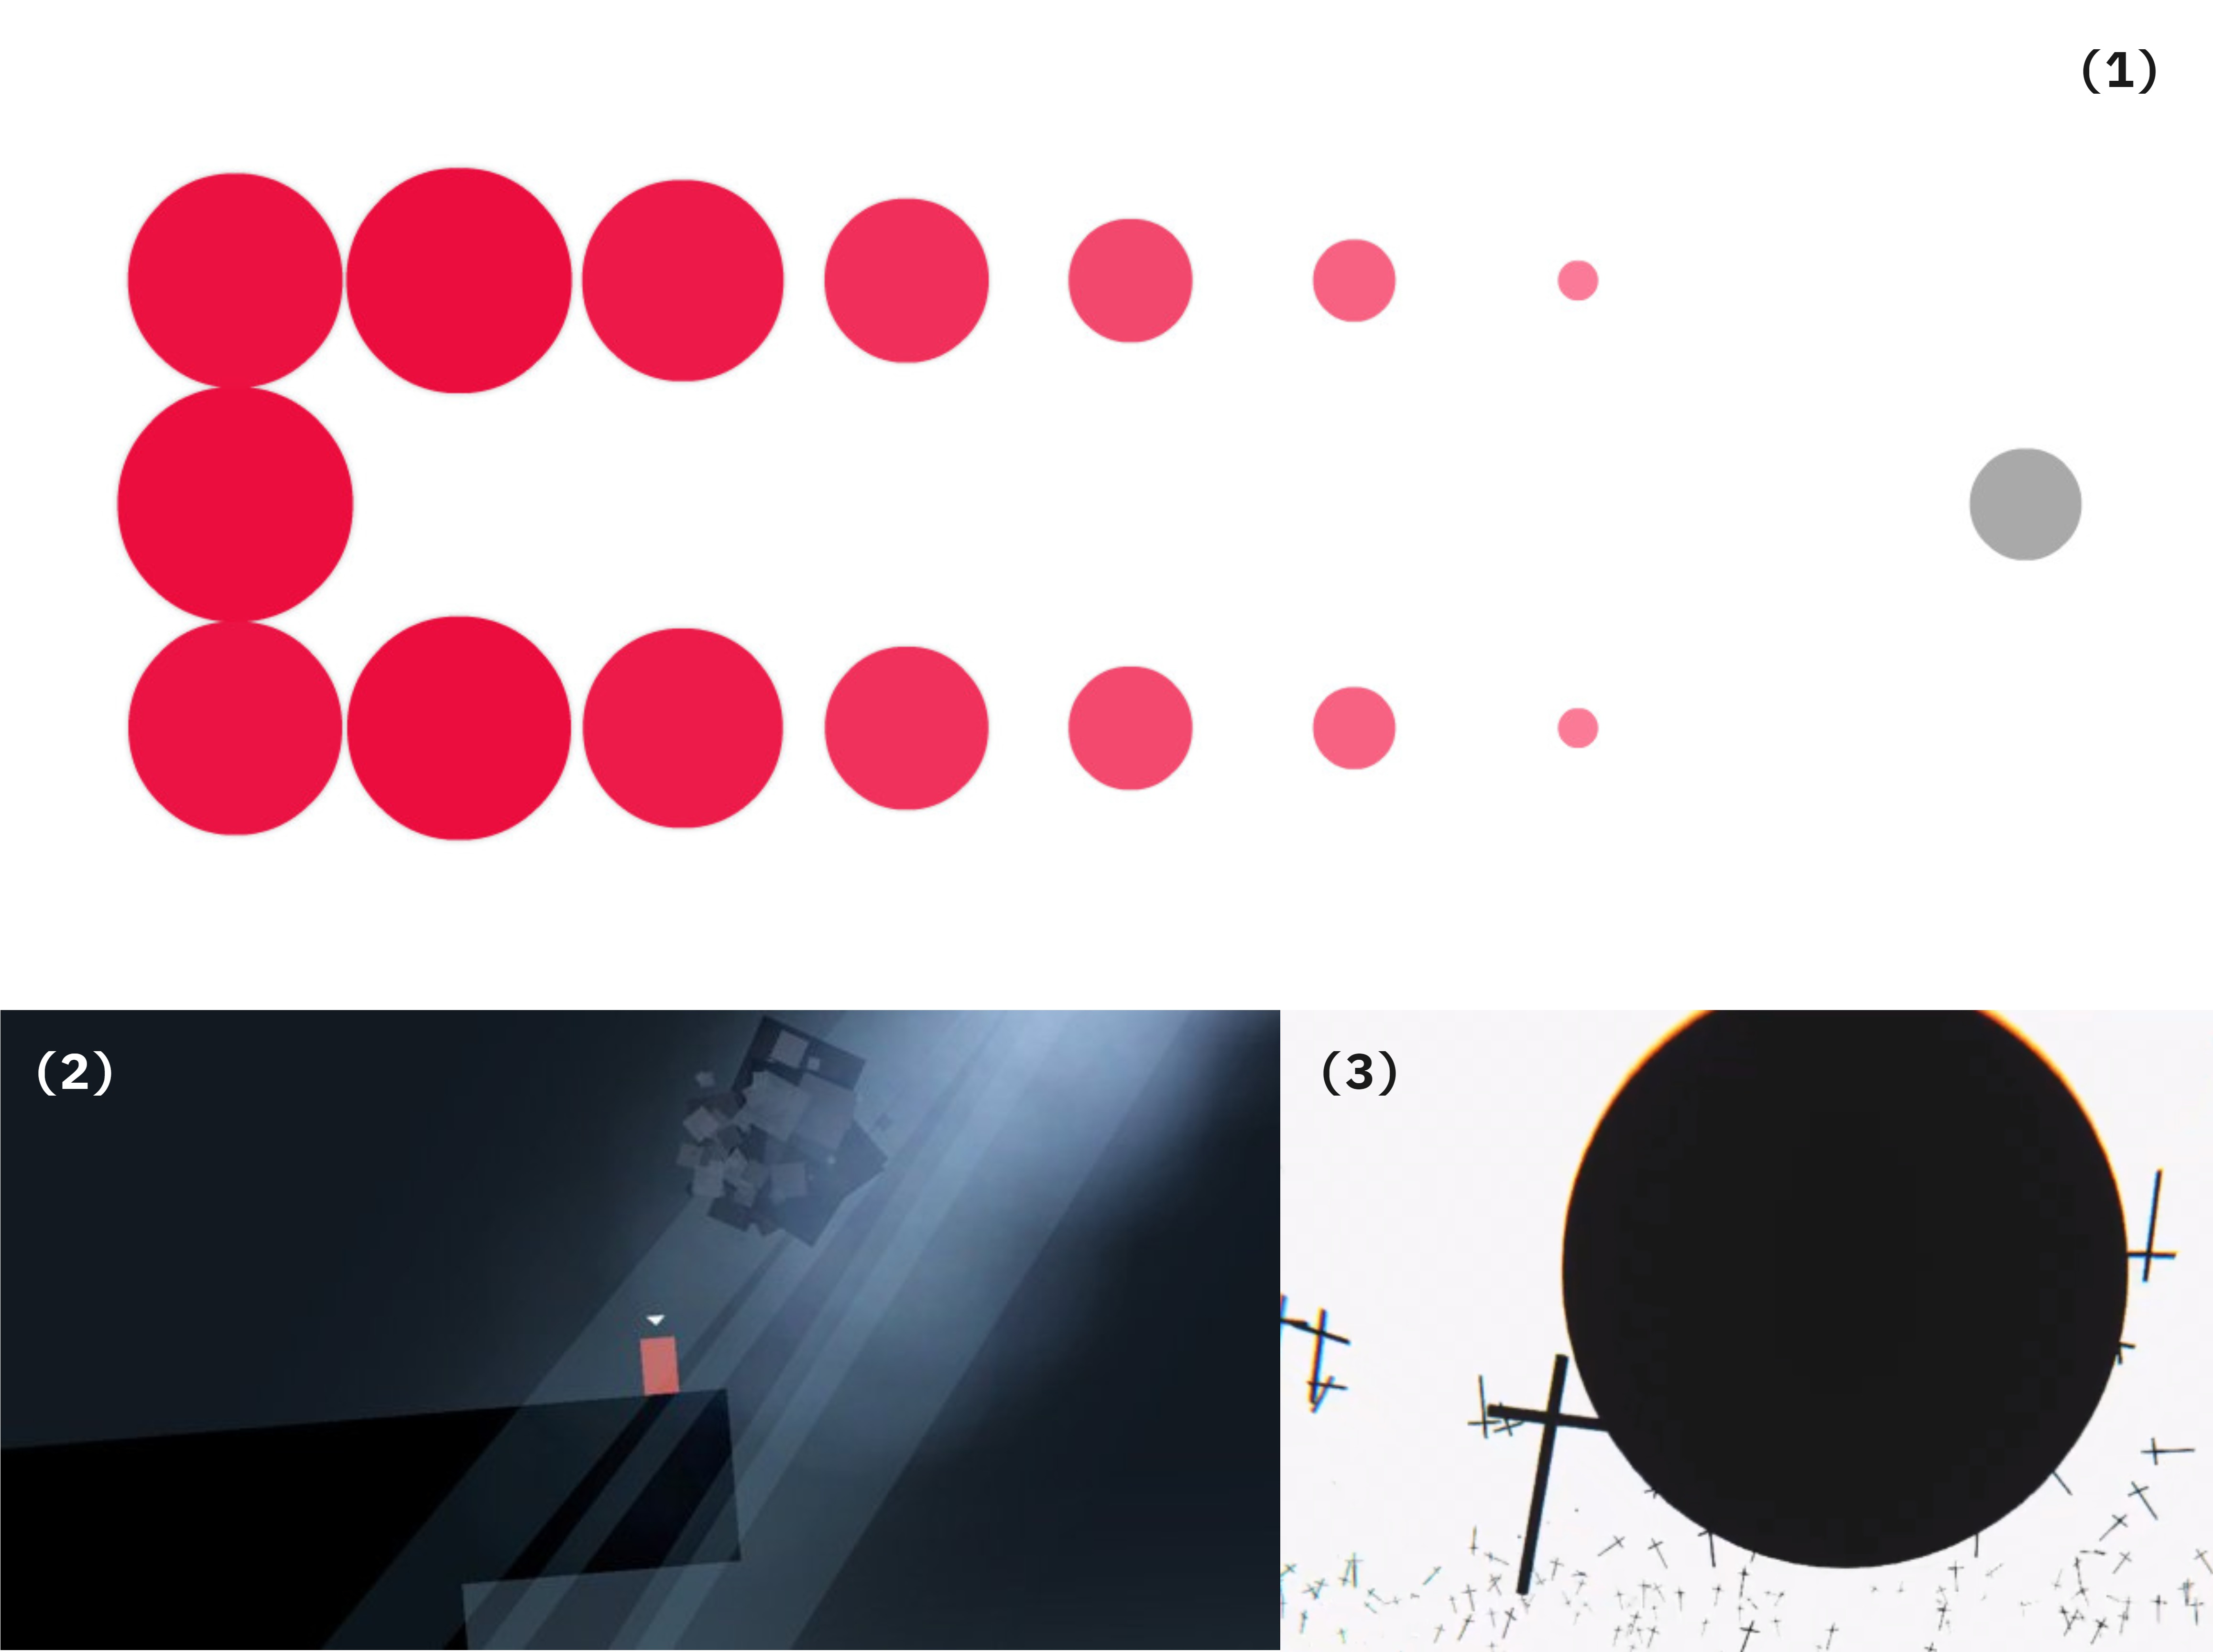
\includegraphics[width=\textwidth]{probeinspiration.jpg}
  \caption{Probe aesthetics inspiration (including \textit{Circles} \cite{circles2017} by Jeroen Wimmers (1), \textit{Thomas Was Alone} \cite{thomas2015} by Mike Bithell (2), and \textit{Carthasis} \cite{dribble2021} by Oleg Frolov (3))}
  \label{fig:probeinspiration}
\end{figure}

With the general aesthetic direction decided on, the next step revolves around developing a world within which the probe features can be implemented. This game world consists of the game objects representing the different, discoverable objects, a character the player controls, and the background setting. The background setting is going to be kept as minimal as possible, in order to achieve the goal of a minimal, ambiguous but explorable setting for the player. The overall color scheme should strengthen these goals as well. Therefore, a monochrome color palette, with only shades of red as the accent color is used throughout the probe. Concerning how the actual objects within the game world look, these are also visualized as simple as possible, similar to how \textit{Circles} \cite{circles2017} is built. Rather than creating a visually intricate design, playfulness comes from the interaction and from how the objects behave. All of the objects within the game world and their designs can be seen in \textit{Figure \ref{fig:probeobjects}}.

\begin{figure}[h]
  \centering
  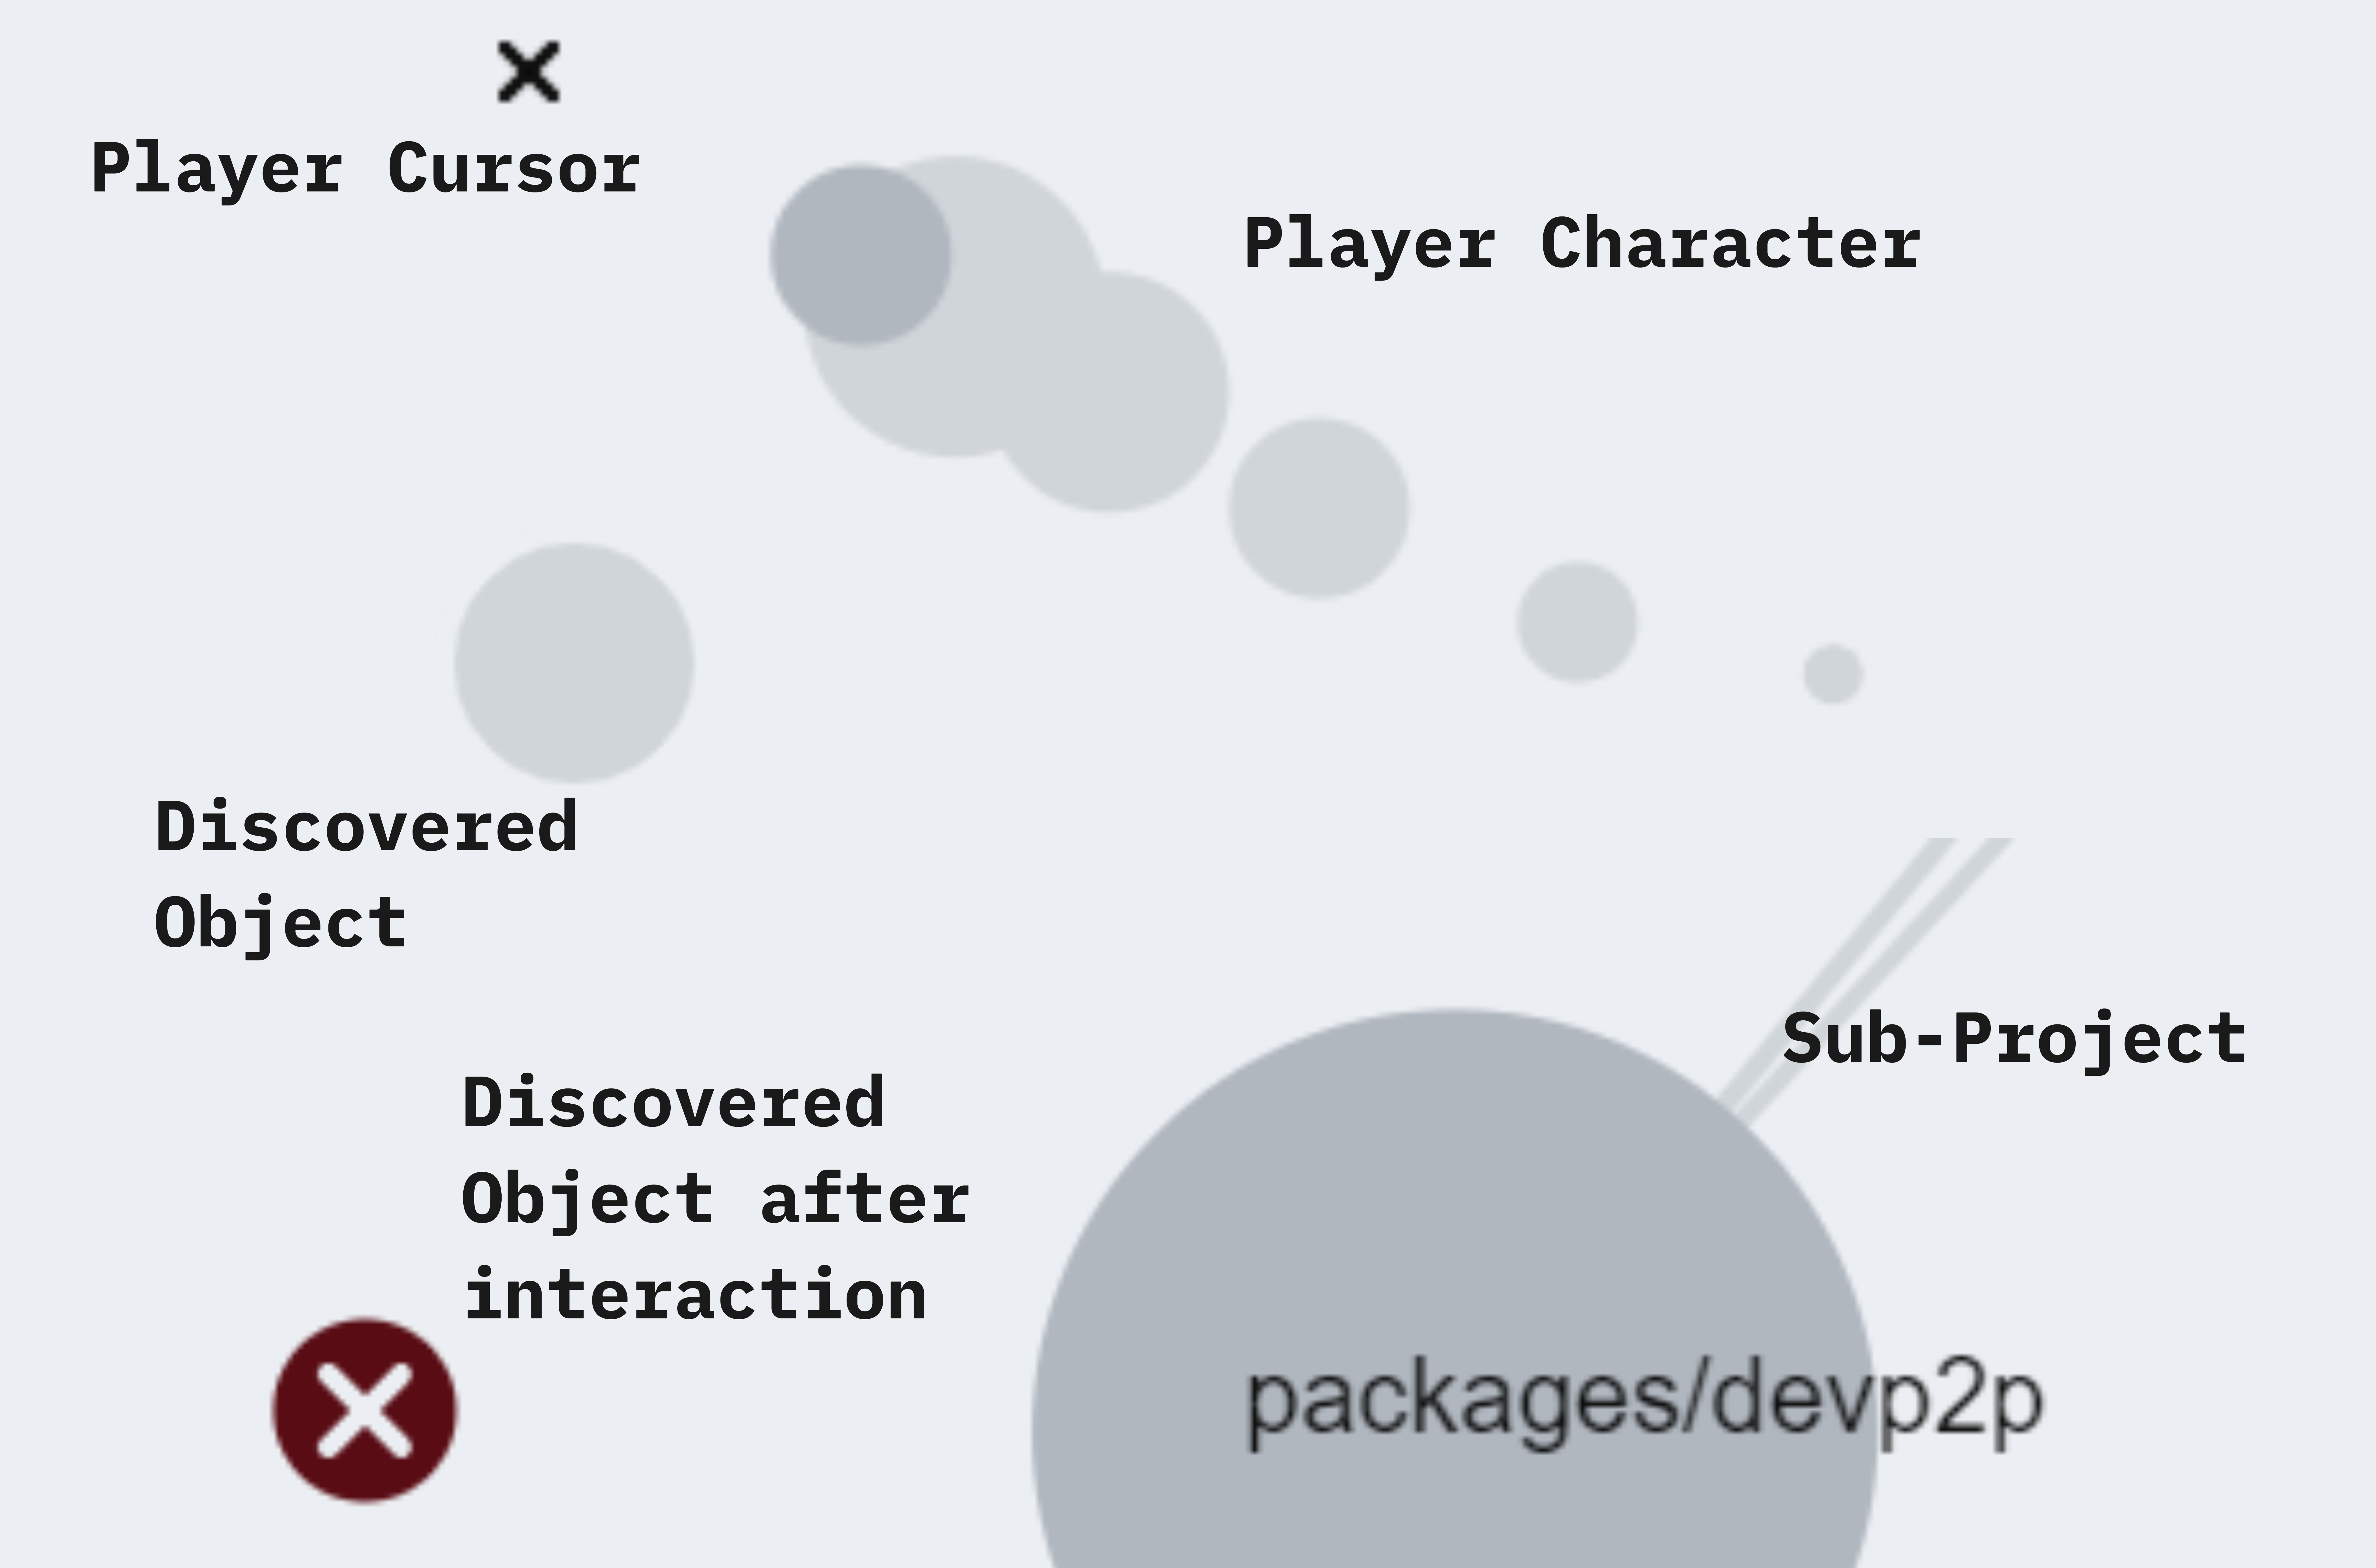
\includegraphics[width=\textwidth]{probelements.jpg}
  \caption{Game objects used throughout the technology probe}
  \label{fig:probeobjects}
\end{figure}

With the main game objects, the color scheme, the overall aesthetic direction, and the features out of the way, the actual implementation can be undertaken at this point. In order to do this, the technical foundation has to be decided on. As mentioned before, the probe is going to be implemented as a web page, therefore the technology choice is limited to that space. Nonetheless, there is a huge variety of possible frameworks in that technology space to choose from. From entire game engines \& frameworks to using no framework at all and relying on \textit{Javascript, \gls{html},} and \textit{\gls{css}} alone.

Using no framework at all -- especially when implementing a highly graphical and interactive application -- presents the need to re-implement a lot of features frameworks provide, like easy interaction handling, animation support, and more. On the other hand, a complete game engine brings much more than is needed in this case. Due to the minimalistic visualization, there is no need for complicated physics replication or support for intricately designed sprites.

A framework that sits in between those two extremes, is \textit{p5.js} \footnote{\url{https://p5js.org/}, accessed on 12th of August 2021}, a \textit{Javascript} implementation of the popular \textit{Processing} \footnote{\url{https://processing.org/}, accessed on 12th of August 2021} framework. It excels in creating interactive visualizations, especially when based on geometric shapes. Combined with my previous experience using this framework, it presents a suitable choice for the implementation of the technology probe.

In addition to that, there are more libraries used for different parts of the implementation to speed up the development. As a build tool, that helps bundling and transforming the written source code into a browser-compatible package and allows usage of \textit{Typescript} \footnote{\url{https://www.typescriptlang.org/}, accessed on 13th of August 2021}, \textit{Parcel} is used \footnote{\url{https://parceljs.org/}, accessed on 13th of August 2021}. To speed up development of all styling not connected to \textit{p5.js}, \textit{SASS} \footnote{\url{https://sass-lang.com/}, accessed on 13th of August 2021} is used. In order to use a central data store, that houses and distributes the current game state, the libraries \textit{Rx.js} \footnote{\url{https://rxjs.dev/}, accessed on 13th of August 2021} and \textit{zustand} \footnote{\url{https://github.com/pmndrs/zustand}, accessed on 13th of August 2021} are used.

Other important helper libraries, include \textit{anime.js} \footnote{\url{https://animejs.com/}, accessed on 13th of August 2021} for animations outside of the interactive visualization, \textit{Moment} \footnote{\url{https://momentjs.com/}, accessed on 13th of August 2021} for date manipulation, \textit{Lodash} \footnote{\url{https://lodash.com/}, accessed on 13th of August 2021} for general utility functions and \textit{Firebase} \footnote{\url{https://firebase.google.com/}, accessed on 13th of august 2021} as a way to persist logging information and answers to the questions accompanying the probe. For the full list of all 3rd-party packages used throughout the probe, refer to the \verb|package.json| \footnote{See suppl. repository at path: \texttt{./technology-probe/package.json}}.

All of these technologies serve the goal of creating the technology probe in the end. This creation itself can be divided into the already defined features, starting with the implementation of \textbf{visualizing the overall project structure}. This overall project structure is defined through the subprojects of the monorepo at hand. How the actual subprojects are programmatically read is the subject of the next chapter. Important to note at this point is the fact that this overview represents a distinct scene within the probe. Meaning, it is a separate view, where only the overall project structure is shown.

To explore the contents of such a subproject, the game objects within this \textit{overview scene} have to be interacted with, leading to a scene change to the subproject's \textit{detail scene}. Within the \textit{overview scene}, the game objects representing the subprojects are placed randomly onto the empty background (as can be seen in the respective file in the source code \footnote{See suppl. repository at path: \texttt{./technology-probe/src/scenes/OverviewScene.ts}}).

To avoid too many game objects overlapping each other, the screen space is divided into sections according to the number of subprojects, within each of those sections one subproject game object is then placed. The size of these objects is determined by the size of the subproject, as is going to be described in the following chapter. The initial state of these game objects is shown in \textit{Figure \ref{fig:probeobjects}}. The player character (also shown in \textit{Figure \ref{fig:probeobjects}}), then is able to interact with the subproject objects. Upon collision of the player character with those objects, they grow in size and turn slightly opaque, letting the player still see their character, but also indicating, that interaction with the respective object is possible. Another important visualization shown between these objects themselves is the interconnection between subprojects of the same monorepo. These are indicated with lines connecting the subproject objects. The actual implementation details would go too far into detail, but can be found in the respective file of the codebase \footnote{See suppl. repository at path: \texttt{./technology-probe/src/sketchObjects/Player.ts}}. Where the transition to the next feature of the technology probe happens, is after the interaction -- a mouse click onto a subproject -- with the respective object.

On this click, the \textit{detail scene} containing the information for the respective subproject is shown. Therein it is possible to \textbf{freely explore the subproject} and to \textbf{use a reveal mechanic to uncover objects in subprojects}. Initially, the \textit{detail scene} is void of any visible elements. Uncovering objects within the scene requires the player to use the reveal mechanic implemented within the scene. This reveal mechanic is loosely inspired by what games like \textit{osu!} \footnote{\url{https://osu.ppy.sh/home}, accessed on 13th of August 2021} are doing, where the player moves the character to different points on the screen to reveal and interact with newly appearing circles growing and decreasing in size. In the case of this technology probe, the elements do not show up after a set amount of time, rather through user-induced reveal \enquote{\textit{bubbles}}. These can be spawned at arbitrary points on the screen, growing in size until they fade out after a set amount of time. As soon as a \textit{reveal bubble} is colliding with a currently invisible discoverable object, the discoverable object (as shown in \textit{Figure \ref{fig:probeobjects}}) can be interacted with, similar to the game objects representing the subprojects in the \textit{overview scene}. To better visualize this interaction, \textit{Figure \ref{fig:probedetail}} shows the player character, with a growing \textit{reveal bubble}, revealing underlying game objects.

\begin{figure}[h]
  \centering
  
\includegraphics[width=\textwidth]{probedetail.jpg}
  \caption{Probe detail scenes with discovered object (1) and object ready for interaction (2)}
  \label{fig:probedetail}
\end{figure}

Within that figure, two different scenes are shown, with the first (1) one showing how to reveal bubbles uncover the invisible game objects scattered on the scene. The second scene (2) in contrast, shows how -- as long as the object is within a reveal bubble -- the discovered game objects signify that they can be interacted with. In addition to this reveal mechanic, the discovered objects move randomly across the screen to turn a rather static uncovering experience into a more dynamic one -- amplified by the fact that the discoverable objects only ever are visible during their collision with the reveal bubbles. Again the implementation details -- like the collision calculation between \textit{reveal bubbles} and the discoverable objects -- can be found in the respective files of the accompanying probe codebase \footnote{See suppl. repository at path: \texttt{./technology-probe/src/sketchObjects/Player.ts}} \footnote{See suppl. repository at path: \texttt{./technology-probe/src/scenes/DetailScene.ts}} \footnote{See suppl. repository at path: \texttt{./technology-probe/src/sketchObjects/Revealable.ts}}.

On interaction with those discoverable objects, the nature of these objects is revealed. There are three different types of revealable information important to a newcomer, as discussed earlier: \textbf{The discovery of potential issues, important contributors \& 3rd-party packages used}. Upon interaction with the respective discoverable object, an information message is shown. This message shows accompanying data, depending on the type of revealable information. The actual data that is shown is described in detail in the following chapter as it is directly generated from the underlying project. The visualization of the messages on the other hand is attached to this thesis in \textit{Appendix \ref{append:probe-types}}. The player also gets the option to have a detailed look at the contributor's \textit{Github} profile or a potentially problematic file within the codebase. After the info message was dismissed by the player, the discoverable object is then permanently visible indicating that it has been interacted with (as shown in \textit{Figure \ref{fig:probeobjects}}). Again, the implementation details can be found in the respective source code file\footnote{See suppl. repository at path: \texttt{./technology-probe/src/ui/info.ts}}.

At this point, there is only one last feature to implement, the \textbf{creation of a companion helper}. To be helpful, this companion should guide the player through the intricacies of the probe and provide additional information when needed. Specifically, the companion indicates, when everything is revealed within a subproject and when everything is revealed within the probe as a whole. Additionally, if the player fails to interact with the elements on either of the scenes, the companion presents a message describing the game mechanic needed to accomplish the next step within the probe. To be precise, within the \textit{detail scenes}, if after six seconds no reveal bubbles were spawned, the companion presents a message clarifying that mechanic. After ten additional seconds, if no discoverable object was interacted with, the companion tells the player to click the discovered objects. Within the \textit{overview scene}, if after six seconds no subproject element was interacted with, the companion explains that mechanic as well. In \textit{Figure \ref{fig:companion}} an example is shown of such a helper message.

\begin{figure}[h]
  \centering
  
\includegraphics[width=\textwidth]{companionmessage.png}
  \caption{Helper companion within the technology probe}
  \label{fig:companion}
\end{figure}

Within that figure, attempts on making the companion having more personality are also visible. The companion's pupil follows the player's cursor to make it feel more connected to the player's actions for example. In addition to that, the companion should seem more approachable with friendly facial features, as well as the usage of a friendly tone of text together with the usage of emoticons. If these attributes achieve the goal of a companion with personality, is subject to discussion based on the probing results. For the implementation details of the companion, as well as the full set of companion messages, refer to the probe codebase\footnote{See suppl. repository at path: \texttt{./technology-probe/src/ui/companion.ts}}\footnote{See suppl. repository at path: \texttt{./technology-probe/src/ui/intro.ts}}\footnote{See suppl. repository at path: \texttt{./technology-probe/src/scenes/DetailScene.ts}}.

This concludes the user-facing implementation of the technology probe. The actual generation and size of the scenes as well as the game objects is based on the underlying project's metadata and source code. How the data is programmatically read, what data is used, and how it is integrated into the technology probe, is subject of discussion within the next chapter.

\subsubsection{Game World Generation}

In order to generate a game world from a project's source code and metadata, multiple distinct levels of tasks are necessary. To be more specific, at first, the data that is needed to generate the world has to be defined, based on what outcomes are wished for and what the underlying data can provide. After that, based on the desired data, the location of that data (or the raw data necessary to then aggregate what is needed) has to be identified. The data can then be programmatically fetched from these locations and aggregated into a format that the web page containing the user-facing parts can handle. Based on that data, ultimately the game world, as well as the objects in it can be generated.

% 1. Decide on which data is needed, based on the final implementation

As described, the first step to take is to clarify which data is needed. The most important question to answer here, is: What is the desired outcome? In the case of this technology probe, the data is needed to generate game objects and the overall game world of the technology probe. Therefore, it has to have properties that make it usable for such a generation, like a numeric value that can be used to generate a game object with a distinct size. Additionally, contextual information important for the newcomers can be shown in the mentioned info messages. Based on these constraints the data needed for the different applications throughout the probe is aggregated in \textit{Table \ref{tab:probe-data}}.

\begin{table}[h]
  \begin{tabularx}{\textwidth}{| X | X |}
    \hline
    \textbf{Application}                                   & \textbf{Data Needed}                                                                                      \\ \hline
    (1) Subproject Objects (\textit{Overview Scene})       & Name, Size \& Connections to other subprojects                                                            \\ \hline
    (2) Discoverable Objects (\textit{Detail Scene})       & Size of the object                                                                                        \\ \hline
    (3) Contributor Messages (\textit{Detail Scene})       & (User-)Name, Link to \textit{Github} profile, Last activities within the project, Number of contributions \\ \hline
    (4) 3rd-party Package Messages (\textit{Detail Scene}) & Name, Version Number, Link to package website                                                             \\ \hline
    (5) Potential Issue Messages (\textit{Detail Scene})   & Type of Issue, Issue Location, Link to Issue Location, Size of the Issue                                  \\ \hline
  \end{tabularx}
  \caption{\label{tab:probe-data}Data needed to generate the technology probe game world}
\end{table}

In order to match the contextual information to the in-game world, the size should match the size of the respective subprojects or potential issues. As there is not any directly readable size attribute, an estimation of the size in relation to the other subprojects and issues has to be found. Concerning the subprojects, the most evident correlation would be to the disk space occupied by the respective directory. Concerning the contextual information, some of it can be read directly from the \verb|package.json| files within the subprojects where \textit{Node.js} projects store information about all of the dependencies, both within the monorepo and to 3rd-party packages. Other information, like contributor profiles or their last activities, in contrast have to be requested from \textit{Github}.

Thus, the data can be collected from the following locations. Concerning \textit{application (1)} (refer to \textit{Table \ref{tab:probe-data}} for these applications), the name of the subproject as well as its occupied disk space (=size) and the connections to other subprojects can be read directly from their respective \verb|package.json| file. A \verb|package.json| file does have a standardized schema and includes all 3rd-party packages used in two properties, called \verb|dependencies| and \verb|devDependencies|. Connections within the monorepo are also contained within those properties and marked with a prefix (in this case \verb|@ethereumjs/|).

For application (2) the only attribute needed is its size, as the discoverable objects are randomly placed in the \textit{detail scenes} and are not discernible by type. The size itself depends on the type of object, though, as contributors do have other attributes than 3rd-party-packages for example. Therefore, the size of the respective shape has to be generated based on a different data attribute.

Regarding the objects based on contributors (application (3)), this is going to be the number of contributions, as it is an easily accessible number, available through the \textit{Github \gls{api}}\footnote{\url{https://docs.github.com/en/rest}, accessed on 14th of August 2021}. Further, it also is comparable between the different types of contributors and increases the visual weight of the most important contributors. The other data points needed (name, link to a profile, last activities) can also be easily fetched from the aforementioned \textit{Github \gls{api}}.

Concerning application (4), the 3rd-party-package information messages, the data for the package name, and the currently installed version can be sourced directly from the respective \verb|package.json|. The link to the package website is not as easy to uncover, as it is not documented within the project itself. As a workaround, the link to the package subsite within the \gls{npm} ecosystem is created through combining the package name with the base \gls{url} of the \gls{npm} website\footnote{https://www.npmjs.com/package/PACKAGE\_NAME}.

Lastly, the data concerning application (5) has to be collected and aggregated into what is needed. To do this, a certain type of issue has to be decided upon. There are multiple possible issues, especially in large codebases. To keep implementation efforts at a manageable level, only one kind of issue is going to be scanned for in the project. A possible issue, that is easily discoverable from the source project's files alone, are large files. While not necessarily directly connected to badly written code, such large files can be hard to understand and messy \cite{so2012large} for newcomers. Therefore, the identification of such files could present an angle for communication with existing contributors, or for the creation of issues within the source project's repository -- possibly as way to introduce themselves into a project. With the choice on the type of issue out of the way, the needed data (file location, link to the file location and the size of the file) can be gathered directly from the underlying project.

After clarifying, where the data that is needed can be collected from, the actual collection has to happen. Based on the clarification there are two distinct locations, where data has to be fetched from. Firstly, the codebase's files and directories and secondly \textit{Github's public \gls{api}}. The simplest way to access that information is, to do it locally through a script, that programmatically reads from the file system and accesses the necessary \gls{api}. To stay in the \textit{Javascript} ecosystem, the script is created with \textit{Node.js} and can be found within the technology probe's source code as well\footnote{See suppl. repository at path: \texttt{./technology-probe/scripts/get-metadata.js}}. This script can be executed manually and produces an output file containing all the necessary information needed to generate the game world. This file can also be found in the same repository\footnote{See suppl. repository at path: \texttt{./technology-probe/metadata/project.json}}. This file contains all of that information in a file format (.json) readable by the technology probe's source code, in a format that can be easily used for generating the game world. It includes data that is already aggregated into a format that can be used as-is to generate all the game objects, including the size of the shapes, the textual content shown in the info messages, and the links necessary to lead the player to the actual contributors, packages, and more. This is then directly used within the context of the webpage to generate the game objects. Again, the implementation details can be found in the respective repository\footnote{see page 4 for the accompanying repository URL}.

\subsection{Data Collection}

In addition to the user-facing implementation and the creation of the game world, user-generated data has to be collected. This can then be used to draw conclusions from the probe as a whole and to ultimately answer the research questions. As already mentioned in the methodology chapter, user-generated data is collected in four different ways: \textbf{Capturing demographic information (1), logging participant interactions (2), questions on the underlying project (3) \& questions on the research topic (4)}. For all of these ways, the specific questions -- or logging events for that matter -- have to be defined and implemented.

Starting with the demographic information, this should just give some additional contextual information to the participant's background. The primary goal is to research how developers experience playful elements in software development projects unbeknownst to them. Thus, questions on the professional background of the participants are crucial. The participants are also given the option to give their name and age if they so desire. That concludes the small set of demographic questions to be asked. As said, these are just to give some additional context for the result argumentation and to make sure that the participant is part of the target group. Because there are not going to be any generalizable or representative conclusions, no additional demographic information is asked for. The final set of input from the participant at this stage is presented in \textit{Appendix \ref{append:collect}}.

Regarding the second way of collecting data -- logging user interactions within the probe -- additional considerations have to be made. More specifically, the types of interaction have to be considered and how they are logged within the probe. Firstly, a structure has to be defined on how the single events are logged and distinguish the events from each other. The distinction itself is done through a pre-defined two-character code so that it can easily be aggregated and analyzed if needed. The full table of all the codes used throughout the probe can be found in \textit{Appendix \ref{append:collect-log}}. To give context to the singular events, when logging these, timestamps are included to keep track of when and in what sequence these events happened. Additionally, there is the possibility to add custom text to these events if so needed. Within the probe's codebase, a function was created (see the respective file for the implementation details\footnote{Source code file within the accompanying repository at: \texttt{./technology-probe/src/logger.ts}}, making it possible to track events from within the code. These are then persisted through Google's Firebase \footnote{\url{https://firebase.google.com/}, accessed on 14th of August 2021} service, where for each participant the answers to all questions and the logged events are stored for later analysis.

The third way of collecting data is concerned with getting a sense of how the data about the project is translated into the participant's understanding of those. Therefore, it should consist of questions on what was presented regarding the underlying projects. These questions were based on the metadata collected for the generation of the game world and directly target what was presented.

The final set of questions can be found in \textit{Appendix \ref{append:collect}}. Question (1) is about how vividly the participant remembers the contributors shown, as they are the prime social links of a project. Question (2) is added as a way of finding out if the participants connected the subproject size to the size of the shape displayed in the overview scene. The next question (3) is included as a way to find out if the participant recognizes what the lines between the subproject game objects are trying to visualize and how memorable the overall visualization in the \textit{overview scene} was. Question (4) targets the 3rd-party-packages and if the participant remembers some of the ones that were discovered. The last question (5) is targeted towards how participants viewed the last kind of revealable information, the large files that were identified within the game world generation procedure. This last question also includes the participant's opinion on how they would rate the issue of these large files in terms of the graveness of the issue. While this answer is not strictly confined to the underlying project it is very much connected to the topic of the question. Additionally, it transitions into the questions on the research topic as a whole.

These questions on the overall research topic are also included in \textit{Appendix \ref{append:collect}}. In the following, for each of the questions, reasoning is given on why it was included. Question (1) tries to investigate if the participants themselves subjectively feel like they have learned something on the underlying project. To make sure to get more than just a positive or negative reply, within the question it is explicitly mentioned, that the participant should give an answer on what was learned. Additionally, if the participant did not feel like something was learned, an explicit inquiry into what should have been included is added to the question.

Question (2) tries to expand from the learning or onboarding aspect into the overall subjective experience of the participant exposed to the probe. The question is asked in an open-ended manner in order to get qualitative data based on the participant's experiences throughout the probe. Specifically mentioning parts that were liked or disliked by the participant is also encouraged through the wording of the question.

The following question (3) focuses on a single feature of the probe, that might be of value also in contexts other than the technology probe -- the companion and how the participant experienced it. It also acknowledges that the companion might only have been visible as a status indicator not as a helping feature.

Question (4) opens up again, more towards how the participants would describe their stance towards an interactive visualization (as is the case with this technology probe) for software development onboarding purposes. Additionally, it asks for input on projects that might be adequate for such visualizations and on which projects the participant would want to try them out. For, if the participant expresses that they cannot imagine themselves using something like that, a direct query on what they would use instead is included.

Question (5) completely moves away from playful elements in onboarding and tries to get a personal perspective on how each of the participants usually approach onboarding. Specific cues are given to give the participants a clue on what interesting elements of the onboarding process are.

The question after (6) then is more of an optional question, targeted at developers working on open source projects specifically. As the onboarding in such projects is different from a local on-site team, it is included as a way to gather information about how the nature of the project changes how an onboarding process is done at a personal level.

Question (7) then focuses on the explorative nature of the research done within this thesis. It tries to gather input from the \textit{experts} on the topic, the developers, the participants on how they would integrate playful elements in an onboarding context.

Question (8) builds upon that and asks for two things. Firstly, the general stance towards the usage of playful elements in onboarding processes in order to gather information about developers' stance towards playfulness in their work environment. Secondly, the nature of the project is also included as a way to gather data on how participants would perceive playful elements in different contexts (namely working on open source software vs. commercial products).

In the last formulated question (9) the participants are asked for game mechanics familiar to them, that they would deem valuable as playful elements in onboarding processes. While this is a larger task for the participants, input on that question is very valuable, as it further explores ways of using play and playfulness in onboarding contexts.

Finally, question (10) is included as a space, where the participants can give additional feedback independently of the preceding questions.

Overall, all the questions are open-ended where possible, to gather as much qualitative input as possible. Due to the asynchronous and remote nature of the probe, there is no possibility to immediately query the participant on what was said before, though. Due to this downside of the approach, these queries are included within the question, where possible. Concerning the technical implementation, the questions are logged to \textit{Firebase} and added to the participant's data, together with the demographic data and logged events. How the questions are included within the technology probe as a whole is laid out in detail in chapter 4.6.

\subsection{Participant Selection}

After clarifying how the technology probe is implemented, how the game world is generated, and how the qualitative data is gathered only two aspects of the probe are left before the study can be executed. Firstly, all of the single parts of the technology probe have to be put into a distinct sequence, so that the participants are introduced to the study, can give their consent, go through the probe and finally answer the questions outlined before. This is going to be outlined in the next chapter. Secondly, that sequence has to be gone through by a set of participants, that have to be selected based on a set of requirements.

The single most important requirement is that the probe is executed by participants that are part of the context that should be investigated. In this case, these are software developers of any kind. There is no need to limit the selected participants to a certain group or level of experience, as the topic of onboarding is something every kind of developer is exposed to some degree. On the contrary, to get a wide variety of different responses it is beneficial to have a very diverse set of participants (concerning age, experience, and more). Thus, the only requirement concerning the participants is going to be that they are software developers, either professionally, on a leisurely basis, or nascent ones just starting out in the field. As the study is going to be held remotely and asynchronously, the participants do not have to agree on a fixed date and time but can choose for themselves when they want to take part within the probe.

Concerning the number of participants needed, there is no definite amount of participants needed to reach a representative conclusion. Rather, the number of participants should be enough, that an amount of data is generated that produces a big enough foundation to answer the research questions. This is not tied to a set number of participants, but to the data generated by each participant. To get answers that are diverse enough, a minimum number of participants should be set -- in this case five developers. If, after reaching that number of participants in the probe, not enough data to draw conclusions from is generated, additional participants are going to be asked to take part in the study.

\subsection{The Final Technology Probe}

At this point every part of the probe, the constraints around it, and the desired participants are defined. As mentioned before, the only step left at this point is to create a coherent probe that includes all of the carefully created parts in a structured manner. To recapitulate, these parts are \textbf{An introduction to the study, a consent and data protection form, the interactive visualization of the \textit{@etherumjs} project, the demographic questions, the questions on the underlying project \& the questions on the research topic}. All of that has to be combined into an easily accessible technology probe accessible through a browser on a webpage. Together with introductory messages and further information for the participant, the final structure of the probe is as follows:

\begin{enumerate}
  \item{Introduction message to inform the participant on the study, the goal of the study, and the overall procedure}
  \item{Consent \& Data Protection to follow the research ethics guidelines}
  \item{Demographic questions}
  \item{An introduction to the interactive part of the probe}
  \item{Beginning of the interactive part within the probe overview scene}
  \item{Revealing important parts of the project within the probe detail scenes}
  \item{Questions on the underlying project}
  \item{Questions on the research topic}
  \item{Outro message}
\end{enumerate}

For all of these steps, a separate subpage has been created that can be seen in detail in \textit{Appendix \ref{append:probe-steps}}. The implementation of the view logic to cycle through these steps and the elements and styles of these subpages has been done outside of the interactive \textit{p5.js} application with just \textit{\gls{html}, \gls{css}}, and \textit{Javascript (Typescript)}. Details of the implementation can be found mainly in the two respective files of the technology probe codebase\footnote{See suppl. repository at path: \texttt{./technology-probe/src/ui/intro.ts}}\footnote{See suppl. repository at path: \texttt{./technology-probe/index.html}}\footnote{See suppl. repository at path: \texttt{./technology-probe/styles.scss}}. The companion, that was described in detail in chapter 4.3.1 is ultimately included on the lower right of the interactive part of the probe. In addition to that, a counter was added to the technology probe steps 5 \& 6, so that participants get a sense of their progress within the probes. Additionally, the exploration of the subprojects is limited to three, to limit the amount of time needed to complete these steps of the probe. This concludes the documentation of the design and implementation of the research done within this thesis. The next chapter now focuses on the results \& conclusions drawn from that research.

% Results
\section{Results}

With the study executed and analyzed -- using the methods described in the methdology chapter and following the blueprint laid out in the research design chapter -- the results can now be elaborated on in detail and connected to the research questions of this thesis. This elaboration starts with recapitulating and aggregating the final set of playful design implications discovered in literature. After that the results of the study are described in detail as well. This includes the final number of participants, a contextual description of the participants, and their qualitatively analyzed input supported with the answers on the underlying project and the data logged throughout the probe execution. Finally, these results are set into the context of the research questions, so that these can be answered with what was researched throughout the whole thesis.

\subsection{Playful Design Guidelines}

The foundation for the playful design guidelines were discovered through the state-of-the-art literature research and the literature research on the theoretical grounding of this thesis. The actual guidelines were ultimately created as the first step towards the probe implementation. An excerpt of these implications was mentioned before, and the full set of implications can be found in the respective diagram in \textit{Appendix \ref{append:probe-design}}. The final set of playful design implications therefore can be summarized as follows:

\begin{itemize}
  \item{Use serendipitous effects throughout the context}
  \item{Let the player create freely within a space}
  \item{Let the player change the context and visualize the effects}
  \item{Let the player manipulate and destroy parts of the context and visualize the effects}
  \item{Intentionally let the player see through the cracks of the game world}
  \item{Create a game world from contextual data}
  \item{Humanize the context and generate communication through it}
  \item{Create a stage for the player, where they can explore without too much guidance}
  \item{Use uncertainty \& do not reveal everything to the player}
  \item{Utilize playful elements already present in the context}
  \item{Allow for informal and personal communication with the player}
  \item{Purposefully create mysterious elements}
\end{itemize}

Some of these implications resemble very closely what was discovered in existing literature, some are aggregations of multiple sources done by me. For the specific literature this is based upon, refer to the respective diagram in \textit{Appendix \ref{append:probe-design}} and the reasoning in chapter 2.4. This set of design guidelines is one part of the contributions of this thesis as a whole. It informed the creation of the technology probe outlined in the research design chapter, but could also serve as guidelines for the future creation of other playful designs.

\subsection{Study Results}

With the recapitulation of these guidelines as the foundation of the technology probe, the focus can now shift towards the results of that technology probe. This probe is based on the methods mentioned and discussed about in the methodology chapter and was executed as described within the research design. At first there is going to be an overview of the final set of participants. This is enriched with some general aggregate data computed from logging the interactions during probe execution. After that the results of the interim goals during the qualitative content analysis are presented. Ultimately, an attempt at answering the research questions through interpreting and presenting the results of that analysis is made.

Before that can be done, as mentioned, the set of participants has to be presented. As described in both the chapter on methodology and research design, the only requirement towards the participants is that they are a software developer of some sorts. Therefore, two companies that employ software developers were initially contacted and asked to share the \gls{url} to the technology probe with their software developers. This resulted in five initial participants. As the resulting data was not sufficiently diverse, four additional developers were contacted directly via e-mail and also asked to share the probe with their colleagues. Ultimately, nine participants executed the technology probe, with eight of them finishing the interactive part and five finishing the interactive part as well as providing answers to all the questions. The participants were aged 24 to 36, and the participants professional experience varied from zero to more than 10 years. Professions of the participants also varied in detail, with web and software developers, data scientists and others. The final selection with the specific information on each participant and a participant code, that is going to be used going forward can be seen in \textit{Appendix \ref{append:participants}}.

Overall these eight participants went through the interactive part of the probe in times between 2 minutes 18 seconds and 12 minutes 50 seconds. With the exception of one outlier, around 120 to 180 interactions where needed to discover all the revealables generated for the probes. While these aggregate numbers do not carry much meaning by themselves, they (and the single interactions log data points they are based upon) can be used to add contextual information to the qualitative data gathered throughout the study. An overview of these aggregations for each participant can be found in \textit{Appendix \ref{append:log-aggregated}}.

Concerning the content analysis of the qualitative data, it was executed as described in chapter 3.4. In short, there are four phases to go through with the chosen approach: \textit{Selecting material, creating a category system and coding the content with the specified categories}. As mentioned earlier, selecting the material is trivial in the case of this study. Where additional work was done, is in developing a category system that then is used for coding the material, as described by Schreier \cite[p. 174]{schreier2014ways}. To develop such a system it is crucial to clarify what should be achieved by the analysis. In this case, the ultimate goal is to answer the research questions with the data that was generated. Thus, these categories should serve the goal of coding the material with the research questions in mind. This can be achieved by deductively creating the categories from the research questions and the literature they are based upon. The result of this procedure can be seen in \textit{Table \ref{tab:qa-categories}}.

\begin{table}[h]
  \begin{tabularx}{\textwidth}{| X | X |}
    \hline
    \textbf{Research Question}                                                                                                                                                      & \textbf{Categories}                                                                                                            \\ \hline
    (RQ1) How and which theories \& concepts from research on play can be used in the onboarding process of software development projects and how are developers experiencing them? & Ideas on playful elements for onboarding                                                                                       \\ \hline
    (RQ2) Which playful themes could lend themselves well to evolve software development projects into a spaces of play?                                                            & Experience towards playful probe features                                                                                      \\ \hline
    (RQ3) What are the technical, social and personal intricacies of an onboarding context in software development and how do they influence the onboarding experience?             & Social Onboarding (Aspects), Technical Onboarding (Aspects), Organizational Onboarding (Aspects), Ideas on Onboarding Elements \\ \hline
    (RQ4) How can the identified themes be applied in actual onboarding settings?                                                                                                   & Improvements for implemented features                                                                                          \\ \hline
    (RQ5) How do different kinds of software developers experience playful aspects within an onboarding context?                                                                    & Attitude towards Play in Onboarding, Contextual Considerations                                                                 \\ \hline
  \end{tabularx}
  \caption{\label{tab:qa-categories}Content Analysis -- Category System developed from the research questions}
\end{table}

For each of the research questions at least one category has been created, aiming to synthesize valuable data that can be used to answer these questions. If during the analysis of the coding categories were deemed not concise enough for important units of content, sub-categories were inductively created. More specifically, the category of \textit{ideas on onboarding elements} was added to create a distinction on feature-oriented input by the participants. Additionally, a category on \textit{contextual considerations} has been created, as there has been multiple instances input on how the approach on playfulness changes depending on the onboarding context. These categories as a whole then were used to code the content. Where these codes were not enough to create a meaningful unit of content, contextual units were used. As described in chapter 3.4, these contextual units can be supportive data from the logs as well as the playful features themselves. With that information distinct units of text can be coded and set into context and ultimately interpreted in relation to the research questions.

The actual coding process that came after, was two-fold. At first, units of text that contained important content was marked. As a second step, these units of text were then collected and coded using the set of categories defined beforehand. After creating the two additional, inductive categories, the units were examined again, to adapt categories where needed. The result of this process, with every single coded unit of text together with contextual units -- where applicable -- can be seen in \textit{Appendix \ref{append:coding}}. Throughout the results chapter, if a coding unit is referred to, it is done so by an auto-generated number also present in the table within the respective \textit{Appendix \ref{append:coding}}.

Together with all of the work that has been executed prior -- researching the origins of play, contemporary views, creating design guidelines, implementing features, creating a technology probe -- this finally allows for careful interpretation of everything that was gathered up until this point.

\subsubsection*{(RQ2) Which playful themes could lend themselves well to evolve software development projects into a spaces of play?}

Concerning this research question much of the effort has already been expended. As described in chapter 3.1, the playful themes were discovered through literature research and careful condensing of what was found into foundations for the playful design guidelines. Thus, this can be seen as the answer to the first part of this question. If they lend themselves well in the context of onboarding onto software development projects is unanswered, though. As was mentioned in chapter 3.4 as well, a generalizeable and reliable answer on effectiveness is out of scope in this thesis. Rather, initial feedback on the subset of playful features implemented has been gathered and can serve as guidance for future applications of play in onboarding processes.

Concerning the theme of creating an intentionally ambigious game world for example there were mixed irritated experiences reported by the participants. P1 mentioned here: \enquote{I was a bit confused because I didn't know what to do when I reached the first blank slide}\footnote{Coding Unit Nr. \textbf{1} in \textit{Appendix \ref{append:coding}}}. Regarding P1 this was also supported by the logged interactions, where the participant did not perform any action at all, until the companion showed the help message\footnote{see lines 10-63 in suppl. repository at path: \path{./supplementary-material/raw-probe-data/technology-probe-logs.json}}. Multiple other participants mentioned that as well. P3 also mentioned that it was not clear how the reveal process within the detail scene should begin and that he did not not know how to start in that scene\footnote{Coding Unit Nr. \textbf{44} in \textit{Appendix \ref{append:coding}}}, which also is supported by this participant's logs\footnote{see lines 9040-9090 in suppl. repository at path: \path{./supplementary-material/raw-probe-data/technology-probe-logs.json}}. P8 mentioned some problems with the detail scene as well, mentioning \enquote{I needed some time and the help box to understand, that I was supposed to click somewhere to reveal the information}\footnote{Coding Unit Nr. \textbf{91} in \textit{Appendix \ref{append:coding}}}. Overall it could be assumed, that the large amount of ambiguity, with completely hidden objects may have gone too far. This is even more important when using those elements as a way to gain knowledge. Here small indicators, or evolving objects that initially are shown in a game world, might have resulted in better understanding.

Here the companion feature was very helpful for the participants, though. P1 for example mentioned that \enquote{helper on the bottom was quick to assist, though}\footnote{Coding Unit Nr. \textbf{14} in \textit{Appendix \ref{append:coding}}} and that it \enquote{came to help always at the right time. Good guy!}\footnote{Coding Unit Nr. \textbf{17} in \textit{Appendix \ref{append:coding}}}. This was also mentioned by P3, albeit in a less personal tone\footnote{Coding Unit Nr. \textbf{45} in \textit{Appendix \ref{append:coding}}} and with the notion, that there was no interaction other than the help messages\footnote{Coding Unit Nr. \textbf{48} in \textit{Appendix \ref{append:coding}}} (this was also mentioned by P6\footnote{Coding Unit Nr. \textbf{71} in \textit{Appendix \ref{append:coding}}}). Overall though, the experience towards the companion was very positive and could be a theme worth exploring further in this context.

The reveal mechanic -- spawning bubbles to reveal information -- on the other hand was perceived more mixed. P8 mentioned that it was fun at first, but in the end it got repetitive\footnote{Coding Unit Nr. \textbf{93} in \textit{Appendix \ref{append:coding}}}. P8 also reported problems catching the revealable objects\footnote{Coding Unit Nr. \textbf{93} in \textit{Appendix \ref{append:coding}}}, which can be traced to the logs as well\footnote{see column \textit{Contextual Unit (Logs)} Nr. 93 \textit{Appendix \ref{append:coding}}}. Albeit the technology probe should be kept very simple according to the literature on it, additional or changing mechanics could have helped here.

Other important notations were targeted towards the overview scene. Both P8 and P6 mentioned that the randomly generated overview was pretty chaotic and therefore the structure of the subprojects were hard to see\footnote{Coding Units Nr. \textbf{64, 94} in \textit{Appendix \ref{append:coding}}}. A more structured visualization could have helped here, although P9 specifically pointed out, that it was helpful to see objects for all the subprojects\footnote{Coding Unit Nr. \textbf{116} in \textit{Appendix \ref{append:coding}}}. Mostly positive feedback was gathered towards the aspects of the underlying project\footnote{Coding Units Nr. \textbf{37, 38, 41, 42, 88, 118} in \textit{Appendix \ref{append:coding}}}. It has to be mentioned, though, that especially P1 had mixed feedback\footnote{Coding Units Nr. \textbf{4, 12} in \textit{Appendix \ref{append:coding}}}. Important to note here, might be that P1 -- in contrast to all other participants -- mentioned that contributors \enquote{don't really help me to get started with a project I guess}\footnote{Coding Unit Nr. \textbf{3} in \textit{Appendix \ref{append:coding}}}.

Overall the study reinforced some playful themes, especially the companion with personal communication and help towards the participants. Others, like the extremely ambigious initial detail scene, irritated more than it helped. Crucial to mention here is that with this study setup no definitive assertion can be made on the effectiveness of these features, it only explores personal subjective experiences of the participants -- to possibly inform such studies on subsets of playful themes in the future.

\subsubsection*{(RQ3) What are the technical, social and personal intricacies of an onboarding context in software development and how do they influence the onboarding experience?}

The approach to answering RQ3 is very similar to the previously discussed research question. Regarding this question, a considerable amount of literature exists and was discussed during the literature research part of this thesis. To summarize, there are different schools of approaches towards software development onboarding: Psychology-centered, process-centered \& developer-centered approaches \cite{yates2014onboarding}. These all focus on different aspects of the onboarding process. Technical intriciacies (psychology-centered approaches) can be program comprehension and programming (or similar purely technical) skills. Social -- and organizational -- intricacies include the project setup as a whole (remote vs. on-site, open-source vs. commercial), but also the project members, experiences of colleagues working on the same project, availability of colleagues or organizational and hierarchical structures behind a project. Lastly, personal intricacies are overlapping with both technical and social challenges. These include personal approaches and processes towards onboarding, like information seeking in projects (no matter if it is organizational or technical information) or feature locating within source code. In my opinion creating a solution that spans every aspect of onboarding is near impossible to achieve as it is such a broad topic. Thus, when creating a supportive digital solution, focusing on a distinct approach is crucial, e.g. by deciding on creating something that supports program comprehension or deciding on improving in-project communication, as vastly different intricacies are present depending on the area of interest. For each of these area of interests research already exists, as mentioned in chapter 2. Thus, an extension of the body of work is not necessary in the case of this question. Nonetheless, the literature discussed and knowledge gained is and was valuable as a foundation for the other parts of the thesis. Where it is important to gain new knowledge is to contextualize the answers the participants provided. This is necessary to understand how different personal approaches towards onboarding might influence the attitude towards playfulness in those approaches.

Concerning this research question, data was gathered on three mentioned different aspects (social, technical, organizational) and ideas from the participants towards aspects of onboarding that are of importance. Here the participants reported very different attitudes towards information in onboarding. P1 for example, as mentioned before, deemphasized the importance of contributors in onboarding\footnote{Coding Unit Nr. \textbf{3, 8} in \textit{Appendix \ref{append:coding}}}. Although it has to be noted, that in on-site projects P1 mentions that social contact and direct communication is important\footnote{Coding Unit Nr. \textbf{23} in \textit{Appendix \ref{append:coding}}}. As P1 mentions having not a lot of onboarding occations and 0-1 years of experience as a developer, this can be set in a context, where P1 might either see contributors not as direct colleagues or has more experience with on-site projects. Concerning these on-site projects, there is consensus between the participants that social links might be the most important in onboarding\footnote{Coding Units Nr. \textbf{53, 59, 76, 98, 123} in \textit{Appendix \ref{append:coding}}}.

A lot of technical onboarding considerations were mentioned by the participants as well. The participants reported mostly similar technical approaches to projects. P3, P8 and P9 all mentioned starting at the top-level of a project and then going into the details of single files and features of these projects\footnote{Coding Units Nr. \textbf{51, 56, 99, 122} in \textit{Appendix \ref{append:coding}}}. An important aspect of this initial approach is the access to the project itself, as for example P6 mentioned: \enquote{I try to get access to everything that I need (git, deployment server, ...)}\footnote{Coding Unit Nr. \textbf{75} in \textit{Appendix \ref{append:coding}}}. For P6, the \enquote{first step is always the documentation, if there are problems I google or search through the issue list}\footnote{Coding Unit Nr. \textbf{80} in \textit{Appendix \ref{append:coding}}}. This statement reinforces the importance of existing information on the project, be it within documentation or in 3rd-party forums. Here the project maintainers themselves can allow for a smoother onboarding experience by providing that -- if these are provided in a coherent manner, that kind of structure can be used within playful elements. Concerning the tools that are used throughout the onboarding process, mostly working directly within the \gls{ide} was mentioned\footnote{Coding Units Nr. \textbf{24, 79, 100, 122} in \textit{Appendix \ref{append:coding}}}. A notable addition to that cam from P8, was that the initial code navigation happens on Github (for projects hosted on Github at least)\footnote{Coding Unit Nr. \textbf{99} in \textit{Appendix \ref{append:coding}}}.

Regarding the organizational aspects, not as much input was given. There are two notable exceptions, though. P3 mentioned that it is very helpful to have a structured and well-organized issue list helps in identifying possible issues to start working on\footnote{Coding Unit Nr. \textbf{55} in \textit{Appendix \ref{append:coding}}}. P6 also brought up the fact that additional communication with non-developers might be worthwhile\footnote{Coding Unit Nr. \textbf{78} in \textit{Appendix \ref{append:coding}}}. This -- arguably also social aspect -- expands the onboarding further into non-technical areas, which have not been the focus up until this point.

To get back to answering the research question as a whole, this wide variety of aspects has to be contextualized. Overall, there are different areas in an onboarding process with each having different requirements and problems inherent to them. Thus, these changing requirements, depending on what is to be achieved, have to be kept closely in mind. In the case of this thesis, this meant for example, that the technical onboarding aspects were pronounced and considered in detail. for future approaches, focusing on the social aspects a different approach might be needed on the other hand.

\subsubsection*{(RQ4) How can the identified themes be applied in actual onboarding settings?}

For a subset of themes, this question can be considered answered already, as a possible application has been done as a part of the implementation of the technology probe. Concerning the playful themes and guidelines that were not implemented, possible applications can be subject to future research into that area. In addition to the documentation of the implementation process and thus the answer towards how to apply some of the themes, feedback on these applications was gathered throughout the study. These can inform how those applications could be improved or extended upon.

To be precise, broad input was provided on how existing features could be improved upon incrementally, but also where the current approach was experienced as lacking. Starting with the visualization of the project as a whole P8 mentioned an improved application through suggesting, that \enquote{there could be some moving dots from module to module, depending on how often the module gets imported into another module}\footnote{Coding Unit Nr. \textbf{101} in \textit{Appendix \ref{append:coding}}} and to adapt the visualization to grasp the importance of these modules\footnote{Coding Unit Nr. \textbf{97} in \textit{Appendix \ref{append:coding}}}. This could achieve a more detailed understanding of the underlying project through leveraging more detailed data from within the project itself. Integrating more data within these visualizations was also mentioned by other participants. P3 mentioned that non-technical information should have been included as well, such as the overall functions of the project itself\footnote{Coding Unit Nr. \textbf{43} in \textit{Appendix \ref{append:coding}}}. P6 also proposed presenting more information within the visualization, by proposing a visualization of the project organization structure together with suggestions of who to communicate with\footnote{Coding Unit Nr. \textbf{82} in \textit{Appendix \ref{append:coding}}} and a stronger connection to the project's source\footnote{Coding Unit Nr. \textbf{69} in \textit{Appendix \ref{append:coding}}}. As of smaller improvements to the implemented features, P1 mentioned adding more images and icons to the information on revealable objects\footnote{Coding Unit Nr. \textbf{10} in \textit{Appendix \ref{append:coding}}} and described how the reveal mechanic could be made more enticing, by increasing depth perception through using different colors\footnote{Coding Unit Nr. \textbf{16} in \textit{Appendix \ref{append:coding}}}.

Overall, most of the participants interacted closely with the implemented features and therefore the application of playful themes. Only P6 went through the probe very fast (as can be seen in \textit{Appendix \ref{append:log-aggregated}}) and did provide not that much feedback on game mechanic intricacies or detailed tasks, rather the feedback was targeted more towards the probe as a whole. Nonetheless, on all of the levels of detail, valuable input was gained on possible improvements to applications of play.

\subsubsection*{(RQ5) How do different kinds of software developers experience playful aspects within an onboarding context?}

The last of the (sub-)research questions is then specifically crafted to foray into a non-existing body of research -- the experience and attitude of developers towards playful elements in onboarding processes. The questions created for the probe mirror that and try to generate data on exactly that aspect of the research topic. The study ultimately succeeded in doing so and the participants brought forth many interesting aspects to this topic, that are going to be laid out in detail at this point. This allows for documenting different experiences to what was built by a set of participants with different experiences and professions.

P1 had a very clear opinion on playful elements for themselves and stated \enquote{this kind of visualization isn't the right thing to learn about a coding project. At least not for me.}\footnote{Coding Unit Nr. \textbf{20} in \textit{Appendix \ref{append:coding}}} P1 underlines that by giving an opinion on playful elements in onboarding processes as a whole. More specifically P1 mentions urgency and time available to get to know a new project and states that in time-sensitive situations playful elements hinder effective onboarding\footnote{Coding Unit Nr. \textbf{18, 19, 30} in \textit{Appendix \ref{append:coding}}}. P1 even describes it as potentially \enquote{frustrating}\footnote{Coding Unit Nr. \textbf{19} in \textit{Appendix \ref{append:coding}}}. What P1 also describes is the need for the right time and mindset necessary for a playful exploration of a project, where parts of a project are explored that might not be connected directly to the work done at the moment \footnote{Coding Unit Nr. \textbf{31} in \textit{Appendix \ref{append:coding}}}. An important aspect that P1 also mentions is that playful exploration should be done at a pace individual to the respective developer \footnote{Coding Unit Nr. \textbf{20} in \textit{Appendix \ref{append:coding}}}.

P3's attitude towards playful elements stands in contrast to P1's statements -- at least regarding the general opinion on those playful elements. P3 specifically brings up that a visualization coupled with playful exploration techniques might be able to provide a good \textit{first} overview of a project \footnote{Coding Unit Nr. \textbf{50, 60} in \textit{Appendix \ref{append:coding}}}.

P6 shares these sentiments with specifically pointing out that the playful elements and the exploration could provide a benefit to get an overview of software development projects\footnote{Coding Unit Nr. \textbf{72} in \textit{Appendix \ref{append:coding}}}. P6 acknowledges that this is not true at all times, though, by mentioning the inefficiency of such an approach in day-to-day work\footnote{Coding Unit Nr. \textbf{83} in \textit{Appendix \ref{append:coding}}} and that technical onboarding might better be done through \gls{ide}s and the such\footnote{Coding Unit Nr. \textbf{74} in \textit{Appendix \ref{append:coding}}}. P8 gives similar feedback, with mentioning the possible inefficiencies -- largely caused by the \textit{randomness} of the revealable objects -- of a playful approach\footnote{Coding Unit Nr. \textbf{96} in \textit{Appendix \ref{append:coding}}}. However, P8 also found aspects of the approach helpful, like pointing out potential issues of the underlying project\footnote{Coding Unit Nr. \textbf{89} in \textit{Appendix \ref{append:coding}}}, although that statement is not directly related to a playful approach, rather on the data extracted from the underlying project. P9 points out similar sentiments, albeit targeted more towards projects where getting an overview from the outside just by investigating the source code files might be hard to achieve\footnote{Coding Unit Nr. \textbf{121} in \textit{Appendix \ref{append:coding}}}.

To summarize these findings, there are mixed results on developer experience and attitude towards playful elements in onboarding. While there are statements towards the inefficiency of playful elements, the usage of these elements for getting initial overviews and exploring parts of the project that are not directly worked with, was described positively. Overall the participants reported no fundamental resentment towards play in onboarding processes, but mentioned important considerations and possible downsides of such approaches.

Some of those important considerations are connected to the context in which onboarding takes pace. Aspects of this were mentioned by multiple participants based on the question of playful elements within a work environment and open-source projects. P3 and P8 for example mention that in on-site working environments the access to other project members and experts can be significantly better. Thus direct in-person communication -- which is preferable for the participants -- is easier to achieve. Therefore, both P3 and P8 mention that an automated playful introduction should be more valuable when this in-person communication is not feasible\footnote{compare Coding Units Nr. \textbf{61, 62, 107, 109} in \textit{Appendix \ref{append:coding}}}. P6 and P8 also mention the motivation behind working on open source projects (\enquote{out of interest}\footnote{Coding Unit Nr. \textbf{84} in \textit{Appendix \ref{append:coding}}} or in a \enquote{self-motivated}\footnote{Coding Unit Nr. \textbf{108} in \textit{Appendix \ref{append:coding}}} way), which could increase the openness towards exploring playfully to learn and gain knowledge on a personal level -- rather than focusing on only what is needed to work on specific tasks. P6 also points out that playful approaches might be valuable for young developers or people starting out with development\footnote{Coding Unit Nr. \textbf{85} in \textit{Appendix \ref{append:coding}}}. Lastly P9, adds a another contextual consideration not strictly confined to open source projects but important nonetheless. P9 mentions that in large software projects that are hard to grasp, playful elements and exploration techniques could provide value\footnote{Coding Units Nr. \textbf{121, 124} in \textit{Appendix \ref{append:coding}}}. P9 also specifically points out that this could be helpful for projects built with programming languages the developer is not proficient in, but wants to learn for themselves\footnote{Coding Unit Nr. \textbf{44} in \textit{Appendix \ref{append:coding}}}.

\subsubsection*{(RQ1 -- Main RQ) How and which theories \& concepts from research on play can be used in the onboarding process of software development projects and how are developers experiencing them?}

After answering all the sub-research questions an answer for the overall main research question has to be crafted. Such an answer requires considering the answers to all the previous RQs, additional information from literature, but also all the explorative information generated throughout the study.

In order to use that information on an answer to this question the question has to be split up into its distinct parts: The playful theories \& concepts on one hand and the developers experience towards them. Concerning the playful theories \& concepts in onboarding processes a lot of results have already been generated through the explorative research that happened. This is now enriched with the analyzed study data, where possible. Regarding the second part of the question, this mostly was answered through RQ5.

As said, a lot of different possibilities of which playful theories \& concepts could be applied in an onboarding process has already been explored, which is described in detail in the answer to RQ2 and RQ4. During the analysis of the participant's answers multiple new ideas possibly worth exploring were mentioned. These can be summarized as follows:

\begin{itemize}
  \item{Creating a coherent \textit{quest line} with communicated sub goals to provide a diverse set of actions and mechanics to follow\footnote{Coding Units Nr. \textbf{26, 27, 33, 36} in \textit{Appendix \ref{append:coding}}}}
  \item{Make the participants solve problems, where the solution has to be found by the participants\footnote{Coding Unit Nr. \textbf{32} in \textit{Appendix \ref{append:coding}}}}
  \item{Set up a competition between project members to create additional motivation to find certain elements\footnote{Coding Unit Nr. \textbf{63} in \textit{Appendix \ref{append:coding}}}}
  \item{Explore a story with command line operations\footnote{Coding Unit Nr. \textbf{28} in \textit{Appendix \ref{append:coding}}}}
  \item{Place the companion directly within the working context, e.g. within an \gls{ide}\footnote{Coding Unit Nr. \textbf{81} in \textit{Appendix \ref{append:coding}}}}
  \item{Adding more common game mechanics, like fighting enemies (e.g. software bugs)\footnote{Coding Units Nr. \textbf{103, 105} in \textit{Appendix \ref{append:coding}}}}
  \item{Visualizing the project history\footnote{Coding Unit Nr. \textbf{106} in \textit{Appendix \ref{append:coding}}}}
  \item{Creating a character that follows the player within the game world\footnote{Coding Unit Nr. \textbf{112} in \textit{Appendix \ref{append:coding}}}}
  \item{Implement constraints to the explorable area, so that the player can explore these after each other while gaining knowledge in the process\footnote{Coding Unit Nr. \textbf{113} in \textit{Appendix \ref{append:coding}}}}
\end{itemize}

These ideas on playful elements provided by the participants complement what was found in literature already and present further options to explore and implement in the future.

Ultimately, an extensive list of possible design guidelines and playful themes has been created through carefully examining research in play and on software development onboarding. This list has been developed through following different perspectives onto play throughout the history on research into it. This was enriched with valuable input (shown above) from software developers generated through a study. Overall, this non-exhaustive list covers the question of \textit{which} playful elements could be used in an onboarding context. Concerning the how of this main research question in regards to the playful elements, this was answered through implementing a subset of this list and discussed through feedback by the study participants. Lastly, the question of how software developers experience such elements was answered through the study data as well. A critical discussion of these results is subject to discussion in the next chapter.
% Discussion
\section{Discussion}

With results from the study presented and summarized, it is now crucial to critically reflect on the approach, how these relate to other findings in the area and how releveant these findings are. All of this is subject of discussion within this chapter. To start of, the study approach is reflected upon.

% Discussion of results (justification phase): The critical discussion of the technical or analytical work steps is
% presented here and the relevance to innovation is established. Comparisons with other results on similar
% questions in the literature are entirely appropriate (reference to questions and knowledge gaps in existing
% literature on the topic identified in the “Related Work” chapter). Arguments may also be presented here
% concerning social relevance and responsibility with regard to the research question, or it may be placed it in
% the context of an overall social discourse.

\subsection{Reflection on the Study Approach}

This reflection includes reconsidering the methodological choices and research design, discussing the participant selection and overall study results and possible limitations of the study as a whole. In order to do this, the initial research goal has to be compared to what was researched in the end -- this allows for reconsideration of if the goals were achieved overall. As described in the introductory part of this thesis, this overall research goal was to take a first step into research play and playfulness within the onboarding process of software development projects. Due to this intersection of area not being researched, an exploratory step into it has been taken. This means that a broad range of ideas should be generated, but also the attitude of people within the targeted context should be researched. Both of these should be done in order to gather information about if the mentioned intersection of areas is even desired and secondly how such an intersection could be deployed in the context. Thus, multiple different approaches and aspects should be researched rather than quantifiably and objectively investigating a single aspect.

As mentioned before, a qualitative research approach can be considered sensible in this case, as it can be used to investigate beliefs and attitudes. It also can be valuable in investigating views on a focused topic, which is what is needed in this case \cite{10.1093/humrep/dev334}.

More importantly, the actual methods used have to be reflected on different accounts. Firstly, the the creation of the technology probe is critically observed and secondly, the results of the study is reflected on qualitative research quality criteria proposed by Flick \cite[p. 541-549]{flick2018introduction}.

The study design and process was largely defined by the fact that a \textit{technology probe} was used. A definitive upside of this approach that also influenced the outcome of the study was the fact that participants were directly confronted with a possible implementation of what was discovered in literature. This allowed for a more focused and structured data inquiry, which ultimately led to a large amount of data generated on the selected approaches as well as the overall attitude to playful helpers. A possible downside would be the fact that the participants could have been influenced by what they have already experienced and thus did not get the chance to freely think about possible other approaches to the topic. To gather valuable input nonetheless, the probe was rooted in already existing research on play. This allowed for an informed foundation of the probe, so that the participants answers could be set into the context of the guidelines and features crafted before.

Regarding the selection of features implemented in the probe, there could have been a myriad of other possible designs. Here some kind of pre-selection through either literature or initial feedback from a very small set of developers could have been valuable. It has to mentioned though, that implementing multiple different designs in separation, just to select a subset of features, would have been out of scope of this thesis. Rather the interactive part of the probe itself can be seen as a possible implementation of a subset, that can be expanded upon through future research.

Concerning the combination of qualitative, problem-focused questions, there are some lessons learned though. Rather than including the questions as a separate step after the interactive part of the probe, these questions could have been integrated more deeply. Out of the eight participants that finished the probe only five provided the full set of answers -- here well-integrated questions maybe brought forth by the companion could have led to more involvement and more questions answered by all participants. Certainly setting up the study in a remote and asynchronous manner could have decreased the involvement of the participants. As described before in this thesis, this was a compromise due to the current situation, during which on-site studies would have been hard to execute. Nonetheless, it was discovered through the study, that multiple participants could imagine themselves using tools similar to the probe for open-source projects, which often are organized remotely and asynchronously. Thus, the chosen approach was valuable in exploring how developers would react to tooling that reflects such an organization structure. Still, the study is therefore limited in significance towards aspects of onboarding present in on-site social settings. This presents an opportunity for future research into playfully enhancing those aspects specifically.

Concerning the quality of the study and analysis as a whole, there are multiple criteria the study can be discussed upon. For one, there is the topic of reliability. While this cannot be used similar to how it is used for quantitative studies, procedural reliability is an important aspect of qualitative studies. Regarding the data analysis, this can be increased through reflexive coding and contrasting results against each other. Another important aspect is to divide the data from its interpretation and by documenting the process in great detail \cite[p. 541-543]{flick2018introduction}.

In the case of this study, this is attempted through careful documentation of how the process was taken from literature, extended upon and documenting the decisions needed to arrive at the study setup. Further, all steps connected to data were documented in great detail, as can be seen in the respective appendices and the repository containing supplementary material. The coded data can be clearly traced back to its source with every transformation documented. Additionally, a two-step approach to coding as well as for developing the category system tries to further increase the reliability through incrementally adapting coding units and categories. This documentation also tries to increase the validity of the results through making the research process as transparent as possible \cite[p. 546]{flick2018introduction}. It has to be noted though, that the onboarding done within the technology probe does not fully reflect an actual onboarding setting, as it was specifically crafted as part of the probe. Researching that onboarding context in greater detail, would have required a more observational approach, though. However, this would have not allowed for investigating possible applications of playful themes from literature or inquiring developers on their attitude towards play in their context. This would have to be done in separate steps removed from observation of the setting, rather than doing it within a coherent probe, that provides broader results.

Overall, the study and preceding literature research achieved the goals set in the beginning. Due to its very broad setup, though, the results are limited in their specificity towards single aspects of the process. Thus, the prime motivation of future research should be in gaining more detailed knowledge on specific aspects of playful elements in onboarding processes -- e.g. through focusing on the social structures of projects and how they could be made more playfully. Additionally, the question of possibly increased effectiveness concerning the learning process in onboarding still has to be answered.

\subsection{Related Work}

At this point the results of the study have to be contrasted to the related work researched on in the beginning of this thesis. As this thesis tries to combine multiple different lines of research, this has to be done from multiple angles: The relation to other research on play and to software development with a focus on onboarding onto new projects.

Starting with the relation to play, multiple aspects of playful designs have been mentioned throughout literature research, three of which are reflected upon at this point. Firstly, there is the question of how the playful implementation during the study relates to other playful designs.

% -> Relation to what play is described at -> how playful is it really? -> Would have been a tried and tested game better as the implementation quality is not at question -> Plaful Probe

% -> Relation to other playful designs -> most similar to Bogost's educational tools and explorative case studies brought forth by Sicart e.g.

% -> Relation to gamification -> You could use progress reminders, badges, ... as part of the process to increase engagement !!! but overall they are still not what makes play enjoyable and therefore only should be used in combination with playful elements

% ----------------------
% software Devlopment / Onboarding:
% Yates -> not something that specifically tries to increase efficiency towards feature location and pulling information => Rather an educational tool
% Example with tool to answer questions -> Less focused on efficiency, rather on motivating through the process
% Enjoyment, developer happiness important -> could they increase that - Open for discussion

% ----------------------
% Overall, there is a place for this kind of approach in research -> As play is something that developers seem open towards -> CITE

% Ultimately in relation to other work this study opens up new possibilities not explored until now and simultaneously hopes to inform future research

\subsection{Relevancy \& Future Implications}

% Possible other implementations:
% 
% List here everything that was not done in the probe, but that came up as an idea and put it out there for future research ,e.g.
% 
% - Tell a story through git commits (e.g. text-adventure style as an additional medium)
% - Procedurally generated game world, where players can destroy parts of a project to see what breaks due to that
% 
% -> And every idea from the participants of the probes
% 
% 
% \blockquote{
%   \textit{Note for feedback}
%   \textbf{This is going to be in this part:}
% 
%   How relevant could all of the research be? Can we start to use it immediately? If not, what has to be done? How could we measure effectiveness in the future?
% 
% }
% Conclusion
\section{Conclusion}

At this point, a theoretical foundation for the research topic at hand has been built, a study was designed, executed and analyzed, and its results were critically reflected upon. During the course of these actions knowledge, data and digital artifacts have been created and an attempt at answering the research questions was made. Valuable insights by developers were collected on their attitude towards playful elements in onboarding projects and initial feedback on possible digital implementations based on literature. To conclude this thesis, its specific contribution(s) are summarized once more and an outlook for future research is given.

\subsection{Contribution}

Within the introduction, the desired contribution was already described -- a combination of theoretical guidelines, a digital artifact and empirical findings researched through that artifact. These contributions could be created throughout the study. The theoretical guidelines were derived from literature on play and playfulness and are laid out in detail in chapter 5.1 with the lead-up described in chapter 2.4 and a graphical visualization shown in \textit{Appendix \ref{append:probe-design}}. These guidelines serve as an element of contribution by themselves but also serve as the foundation for the digital artifact crafted from it -- the interactive part of the technology probe.

\subsection{Outlook}

% Look ahead -> What comes after this thesis

% 1. Further development concerning what was created in this thesis

% 2. Further questions arising from this thesis

% 2.1 In which areas of onboarding could playful elements also be used?
% 2.1.1 How could playful elements support building and discovering social structures in onboarding processes?

% 2.2 Observing developers onboarding in-situ, gathering more data on that to find out at which points of the process, maybe even haptic and tangible games could be introduced (Beyond digital tools, focusing on social strctures)

% 2.3 Which specific benefits could playful elements bring to the table in onboarding? -> Quantitively researching benefits of specific solutions
% Sample contents (figures, tables, abbreviations)
% \section{Samples}

This is a section with samples of possible contents within the master thesis.

\subsection{Citations}

Example as follows \cite{wiki}.

\subsection{Figures}

Example as follows, the figure can be referenced like so: Figure \ref{fig:samples-logo}.

\begin{figure}[h]
  \centering
  
\includegraphics{fhsalzburg}
  \caption{Logo of the University of Applied Sciences, Salzburg}
  \label{fig:samples-logo}
\end{figure}

\subsection{Tables}

Example as follows.

\begin{table}[h]
  \begin{tabularx}{\textwidth}{|X|X|X|}
    \hline
    \textbf{Column Head 1} & \textbf{Column Head 2} & \textbf{Column Head 3} \\ \hline \hline
    Column Cell 1 & Column Cell 2 & Column Cell 3 \\ \hline
    Column Cell 1 & Column Cell 2 & Column Cell 3 \\ \hline
    Column Cell 1 & Column Cell 2 & Column Cell 3 \\ \hline
  \end{tabularx}
  \caption{\label{tab:samples-table}A sample table}
\end{table}

\subsection{Code}

Example as follows. This is inline code: \verb|const code = 'Code';|. And this is is multiline code, it is rather ugly though so maybe just use pictures instead.

\begin{lstlisting}
interface Props {
  title: string;
}

const getProps = (): Props => {
  return { title: 'This is the title'};
}
\end{lstlisting}

\subsection{Abbreviations}

Example as follows, \gls{it} is an abbreviation.

\subsection{Footnotes}

Example as follows \footnote{This is a footnote}.

\subsection{Direct Quotations}

Ipsum dolor sit amet, consetetur sadipscing elitr, sed diam nonumy eirmod tempor invidunt ut labore et dolore magna aliquyam erat, sed diam voluptua. At vero eos et accusam et justo duo dolores et ea rebum. Stet clita kasd gubergren, no sea takimata sanctus est Lorem ipsum dolor sit amet. \cite{wiki}

There are direct quotations with less than 3 lines: \enquote{Lorem ipsum dolor sit amet} \cite{wiki} or with more than 3 lines:

\begin{quote}
  \textit{Ipsum dolor sit amet, consetetur sadipscing elitr, sed diam nonumy eirmod tempor invidunt ut labore et dolore magna aliquyam erat, sed diam voluptua. At vero eos et accusam et justo duo dolores et ea rebum. Stet clita kasd gubergren, no sea takimata sanctus est Lorem ipsum dolor sit amet.} \cite{wiki}
\end{quote}


% List of figures
\cleardoublepage
\phantomsection
\addcontentsline{toc}{section}{List of Figures}
\listoffigures
% List of tables
\newpage
\cleardoublepage
\phantomsection
\addcontentsline{toc}{section}{List of Tables}
\listoftables
% List of abbreviations
\newpage
\cleardoublepage
\phantomsection
\addcontentsline{toc}{section}{List of Abbreviations}
\printnoidxglossary[type=\acronymtype,title=List of Abbreviations,style=list,nonumberlist]
% Bibliography
\newpage
\cleardoublepage
\phantomsection
\addcontentsline{toc}{section}{Bibliography}
\begin{singlespace}
\bibliographystyle{acm}
\bibliography{sources}
\end{singlespace}
% Appendix
\begin{appendices}

  \section{Data Protection \& Consent Form}
  \label{append:consent}

  \subsection*{Information about data protection and declaration of consent}

  Dear participant,

  thank you for your interest in participating in this study on ”Playful Experiences in the Onboarding Process of Software Development Projects”. This study takes place as a part of my master thesis on “Onboarding in Software Development Projects as a Space of Play”. The thesis is written as a part of the new Joint Master "Human-Computer Interaction" of the FH Salzburg and the University of Salzburg. In order to use your personal data, we would need your written declaration of consent. Please, carefully read the following information.

  \subsubsection*{General Study Information}

  The goal of this study is to research how software developers experience playful approaches on the onboarding process into new projects. The results of this study are going to contribute to the research body of both the software development field but also the field of “Play”. From the study results conclusions are going to be drawn about: The openness towards playful experiences in the software development field, possible hurdles on implementing such experiences, the general attitude of developers towards play in the field and the selection of what information to include in onboarding processes.

  \subsubsection*{Overall Study Procedure}

  The participant will take part in a hybrid-study setting. Part of the study consists of going through an interactive visualization of an open-source software project and revealing parts of information within some parts of the project. The other part of the study consists of questions on the visualization and general questions on the intersection of Play and software development. The study can be accessed online and can be finished online without additional work on the participants side. Overall the procedure should take between 15 and 25 minutes.

  \subsubsection*{Rights}

  The participation in this study is voluntary. You may withdraw or stop your participation at any time without incurring any consequences. Moreover, you can request information about the processed personal data at any time, even after the termination of the study (for further information see also Confidentiality and data processing). If you have any questions please contact the study leader.

  \subsubsection*{Risks}

  You do not incur any risks by participating in this study. If you feel uncomfortable during the study you can cancel at any time without giving reasons and without incurring any consequences.

  \subsubsection*{Confidentiality and Data Processing}

  Your data will only be processed within the aforementioned project if you give your written consent. The data is going to be processed via the Firebase platform (https://firebase.google.com/) on european servers. For additional information on their privacy and data protection guidelines visit their documentation at https://policies.google.com/u/0/privacy. The following data is going to be processed within the study:

  \begin{itemize}
    \item{Demographic Information (Name, Age, Professional Background, Years of Experience, Gender)}
    \item{Your actions within the visualization (Timestamps of Clicks and Mouse moves together with the timestamps of certain events)}
    \item{Your answers to the questions that are part of the study}
  \end{itemize}

  After the end of the study, the data is going to be exported from Firebase and the underlying app instance is going to be deleted. This data is going to be kept strictly confidential and is not going to be passed on to further third parties. The data is going to be analyzed and then used within my master thesis. If you only want to be mentioned anonymously in my thesis please indicate so at the bottom. If you are doing that your name and age are going to be hidden in my thesis and your data is only going to be connected to a random ID.

  \subsubsection*{Renumeration}

  You will not receive an expense allowance for participation.

  \subsubsection*{Consent}

  I have carefully read and understood the declaration of consent. Any additional questions were answered to my satisfaction. My participation is voluntary, and I know that I can withdraw at any time, even without giving reasons, without incurring any disadvantages. By clicking on “Agree” below I agree to the processing of my personal data collected for this study and I am willing to participate.

  \subsubsection*{Anonimity}

  I want to participate anonymously (the data is not going to be connected to your name)

  \section{Probe Development Process}
  \label{append:probe-design}

  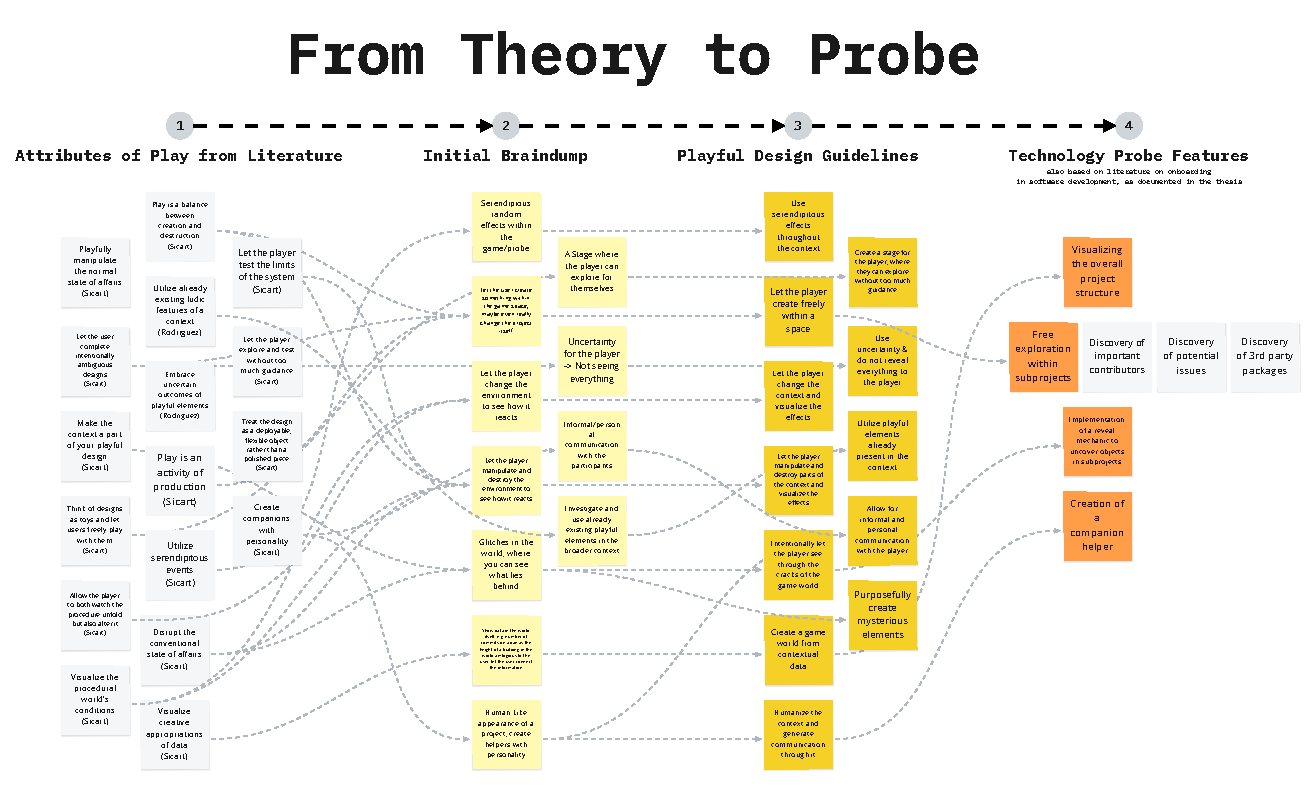
\includegraphics[angle=90,width=0.95\textwidth]{probedesign.pdf}

  \section{Probe Execution Process}
  \label{append:probe-exec}

  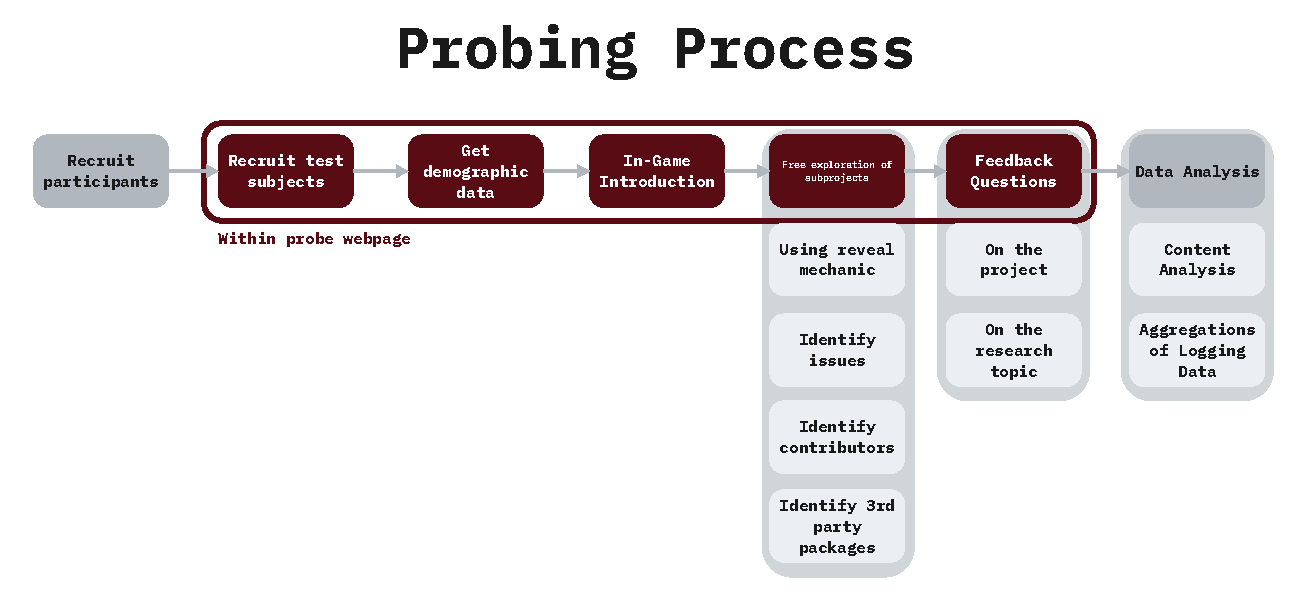
\includegraphics[angle=90,width=0.75\textwidth]{probeprocess.pdf}

  \section{Probe Information Message Types}
  \label{append:probe-types}

  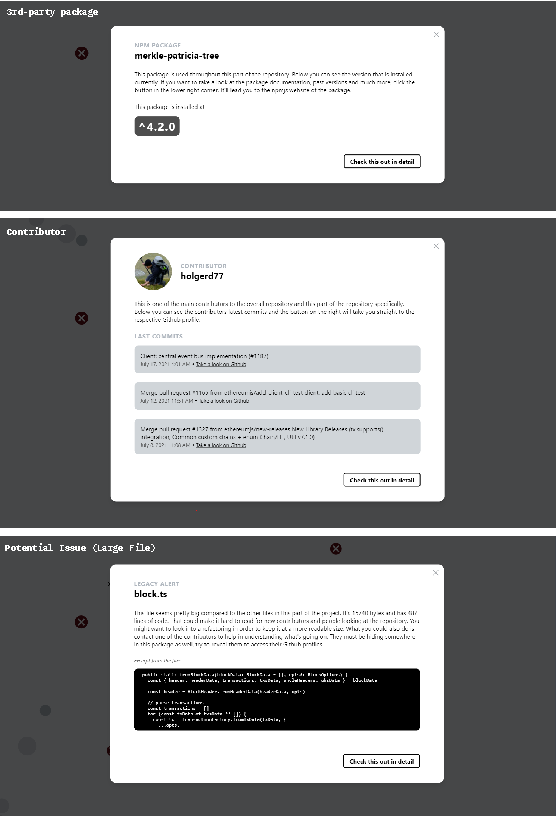
\includegraphics[width=\textwidth]{proberevealables.pdf}

  \section{Probe Data Collection -- Questions}
  \label{append:collect}

  \subsection*{Demographic Information}

  Text Input: \textbf{Your Name}

  Number Input: \textbf{Your Age}

  Text Input: \textbf{Your Professional Background}

  Select Input: \textbf{Your Professional Experience} (Options: 0-1 years, 1-3 years, 3-5 years, 5-10years)

  \subsection*{Questions on the underlying project}

  1) Do you remember any of the contributors of this project? Please name those that you remember below

  2) What were the two largest packages of this monorepo (not the npm packages, but the ones the monorepo is made out of)?

  3) Which of the projects "sub"-packages were used most throughout the other subpackages?

  4) Any npm packages you've revealed in this project, that you can think of? Did you take a look at their respective websites?

  5) Have you taken a look at any of the files that were potentially "legacy" files? If yes, did you agree on them being "refactor-worthy" or do you think they were fine as-is?

  \subsection*{Questions on the research topic}

  1) Would you say, that you have discovered something interesting about the underlying project from going through this interactive visualization? If yes, what? If no, what was missing or what would you have liked to see?

  2) What was your overall experience going through this visualization? What did you like or did not like?

  3) How did you experience the companion (lower right)? Was it helpful, annoying or did you not really interact with it at all?

  4) Could you imagine yourself using some kind of interactive visualization or something similar on different projects to learn about them? If so, on which projects would you want to try it out? If not, what would you prefer instead to make yourself familiar with new projects?

  5) How do you usually approach the onboarding onto new projects? To whom do you talk to, what applications do you use, how do you navigate through code?

  6) Do you work on Open Source Projects? If you are a contributor of one, how do you try to make it easy for new collaborators to work on these projects? If not, how do you approach collaborating for yourself?

  7) Do you have any additional ideas on how playful elements or game mechanics could be used within the onboarding phase of software development projects?

  8) What is your general stance on using games/game mechanics or playful elements within software development? Do you see a difference of using such mechanics in open source software vs. in a work environment?

  9) Do you have any additional ideas on how playful elements or game mechanics could be used within the onboarding phase of software development projects? Any elements from games you play that you think could be reused when making yourself familiar with new projects?

  10) Anything else you want to mention?

  \newpage
  \section{Probe Data Collection -- Logging}
  \label{append:collect-log}

  \subsection*{Logging Single Event Format}

  \begin{itemize}
    \item{\textbf{message}: Additional information depending on the event type}
    \item{\textbf{timestamp}: The unix timestamp at which the event occured}
    \item{\textbf{type}: The type of interaction according to the event codes below}
  \end{itemize}

  \subsection*{Logging Event Codes with their respective interactions}

  \begin{table}[h]
    \begin{tabularx}{\textwidth}{|X|X|X|}
      \hline
      \textbf{Event Code} & \textbf{Interaction}   \\ \hline \hline
      CC                  & Click on companion     \\ \hline
      OC                  & Overview click         \\ \hline
      RC                  & Reveal click           \\ \hline
      LI                  & Legacy identified      \\ \hline
      LR                  & Legacy revealed        \\ \hline
      PI                  & Package identified     \\ \hline
      PR                  & Package revealed       \\ \hline
      NI                  & Contributor identified \\ \hline
      NR                  & Contributor revealed   \\ \hline
      SF                  & Subproject finished    \\ \hline
      GF                  & Game finished          \\ \hline
    \end{tabularx}
  \end{table}

  \newpage

  \section{Technology Probe Scenes}
  \label{append:probe-steps}

  \subsection*{Step 1: Introduction}

  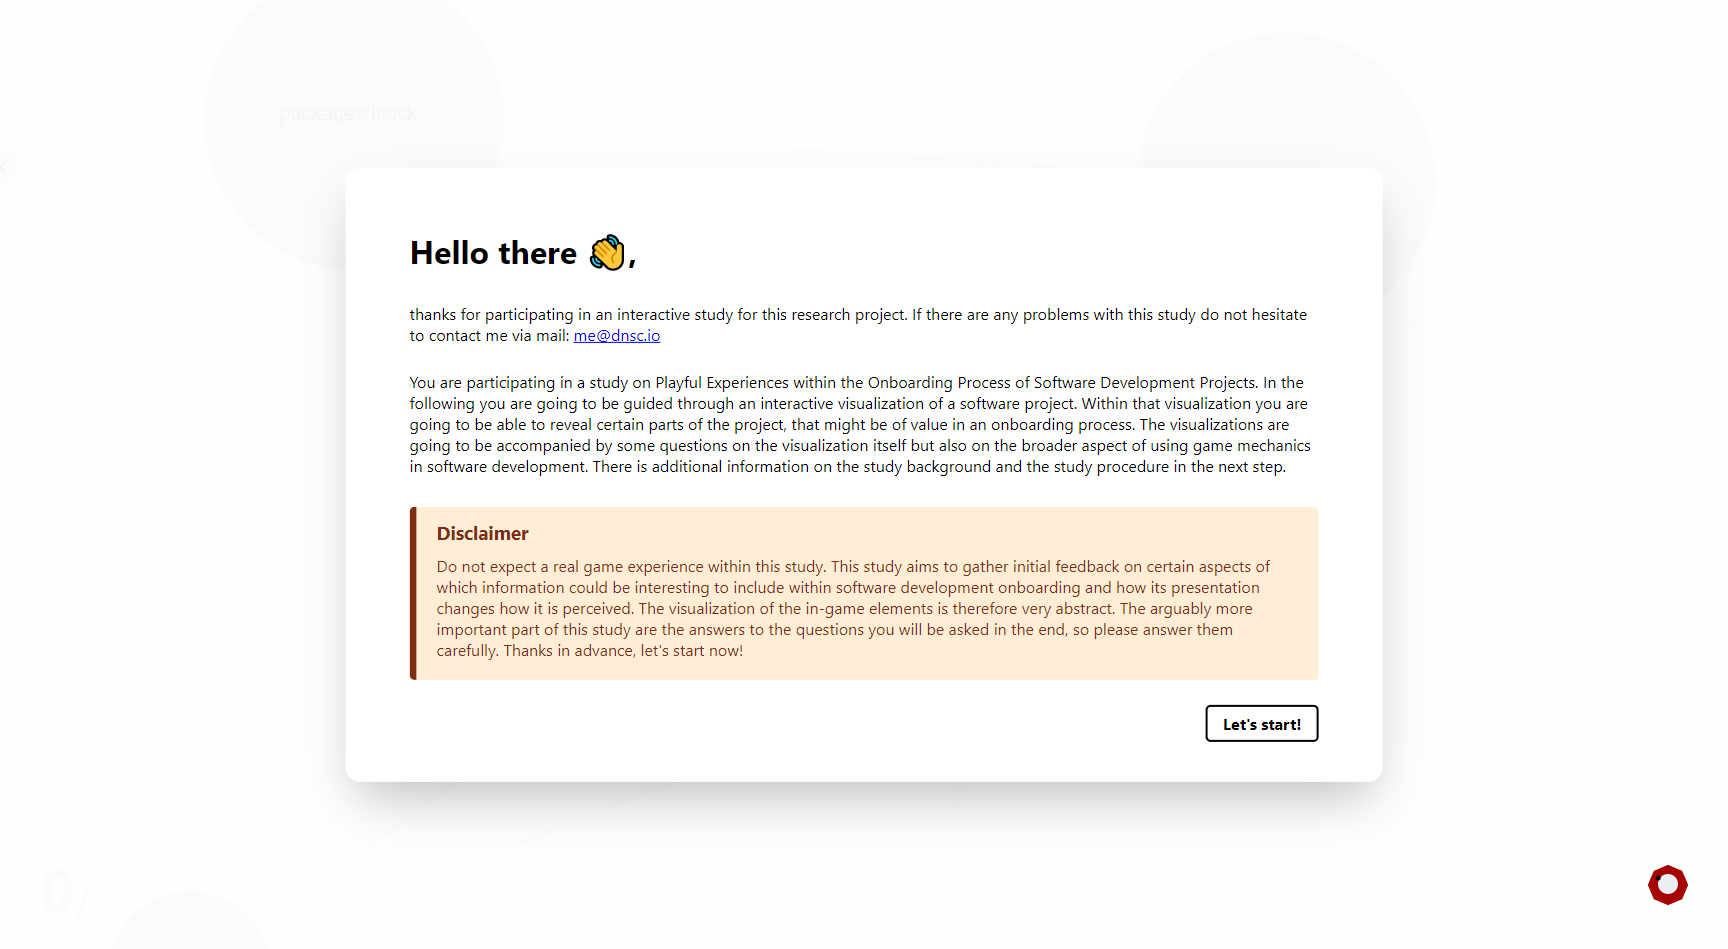
\includegraphics[width=\textwidth]{probesteps/step1.png}

  \subsection*{Step 2: Consent \& Data Protection}

  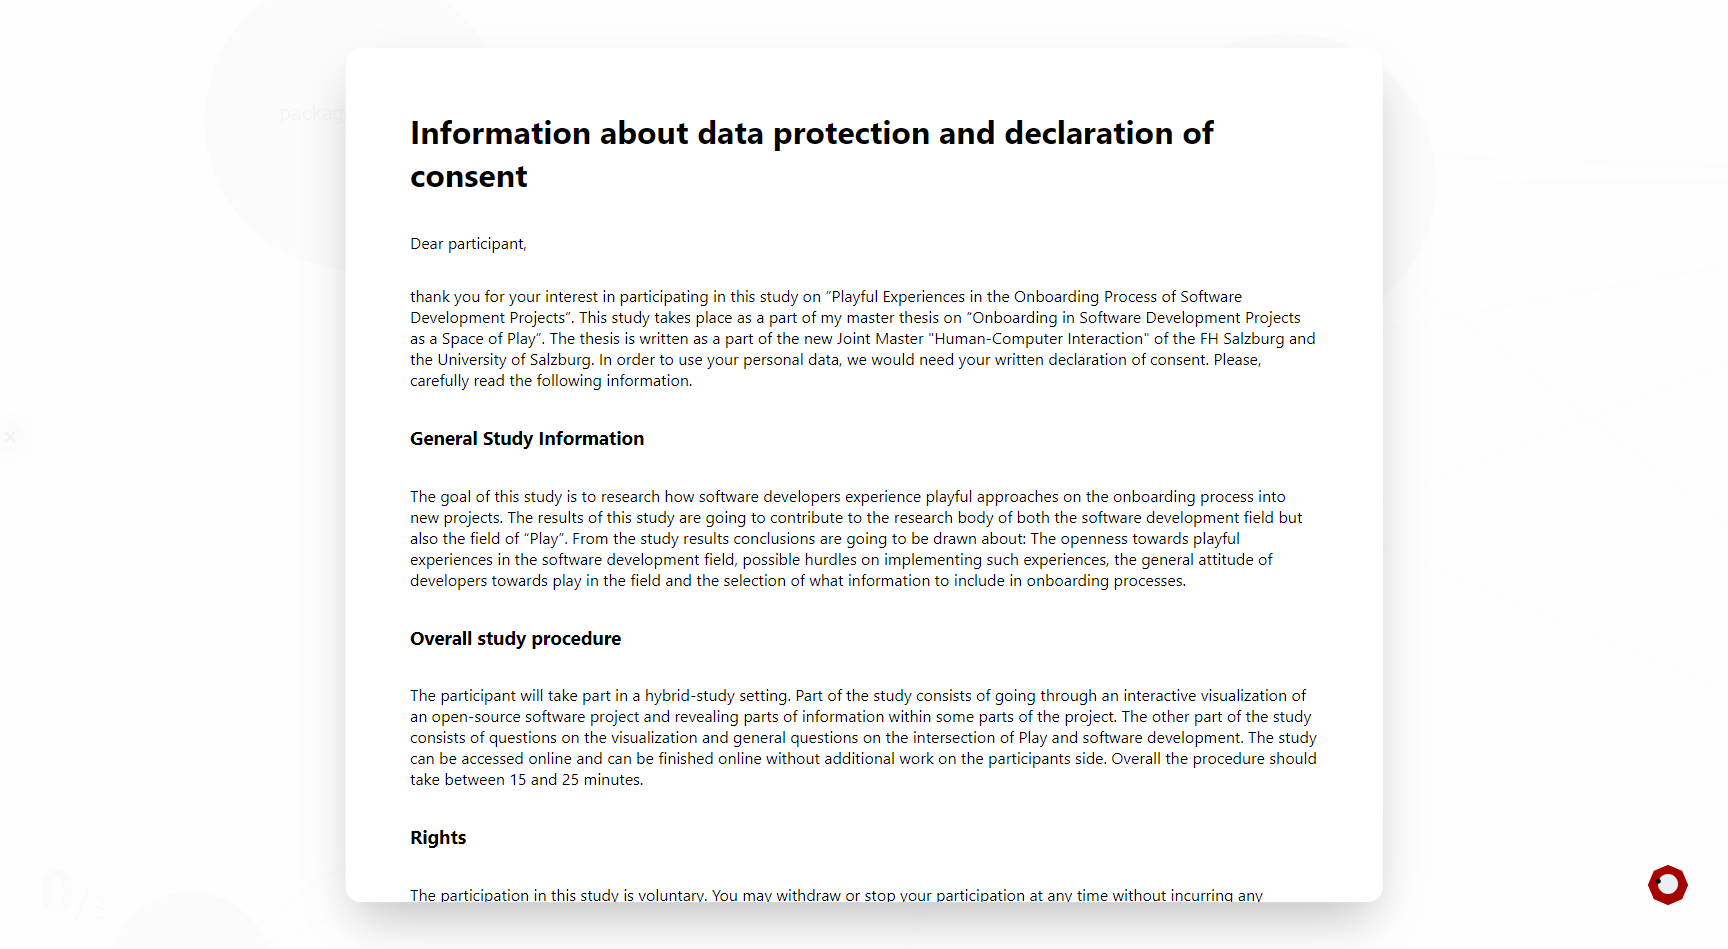
\includegraphics[width=\textwidth]{probesteps/step2.png}

  \subsection*{Step 3: Demographic Questions}

  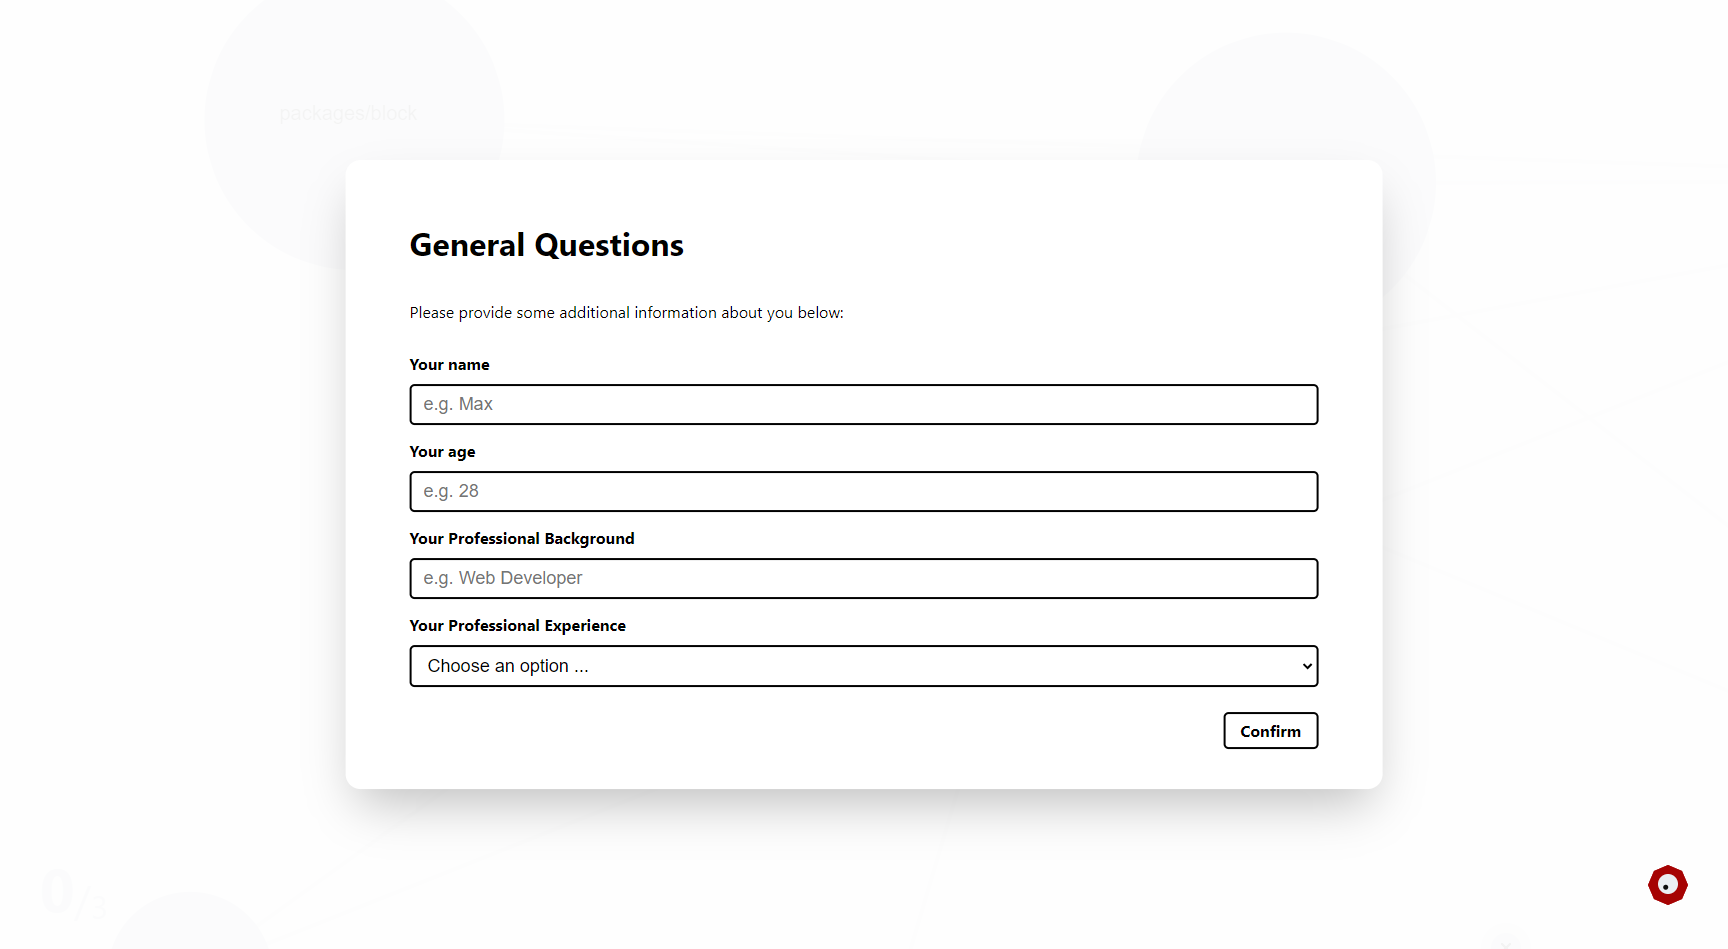
\includegraphics[width=\textwidth]{probesteps/step3.png}

  \subsection*{Step 4: Visualization Introduction}

  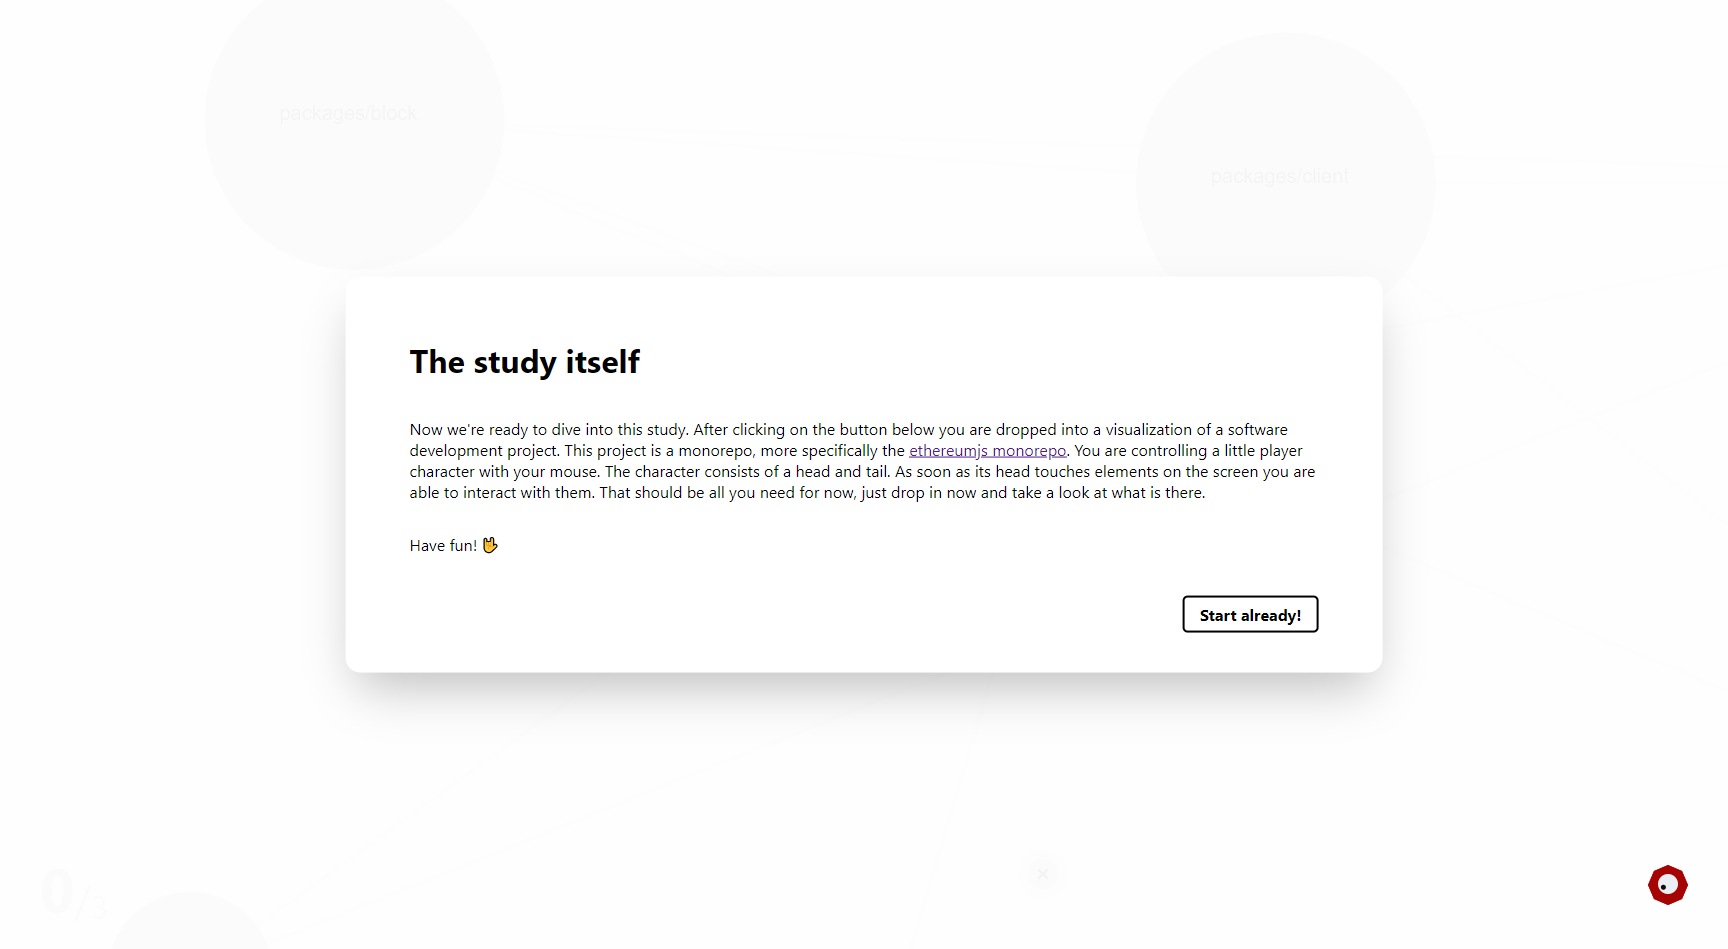
\includegraphics[width=\textwidth]{probesteps/step4.png}

  \subsection*{Step 5: Probe Overview Scene (Example)}

  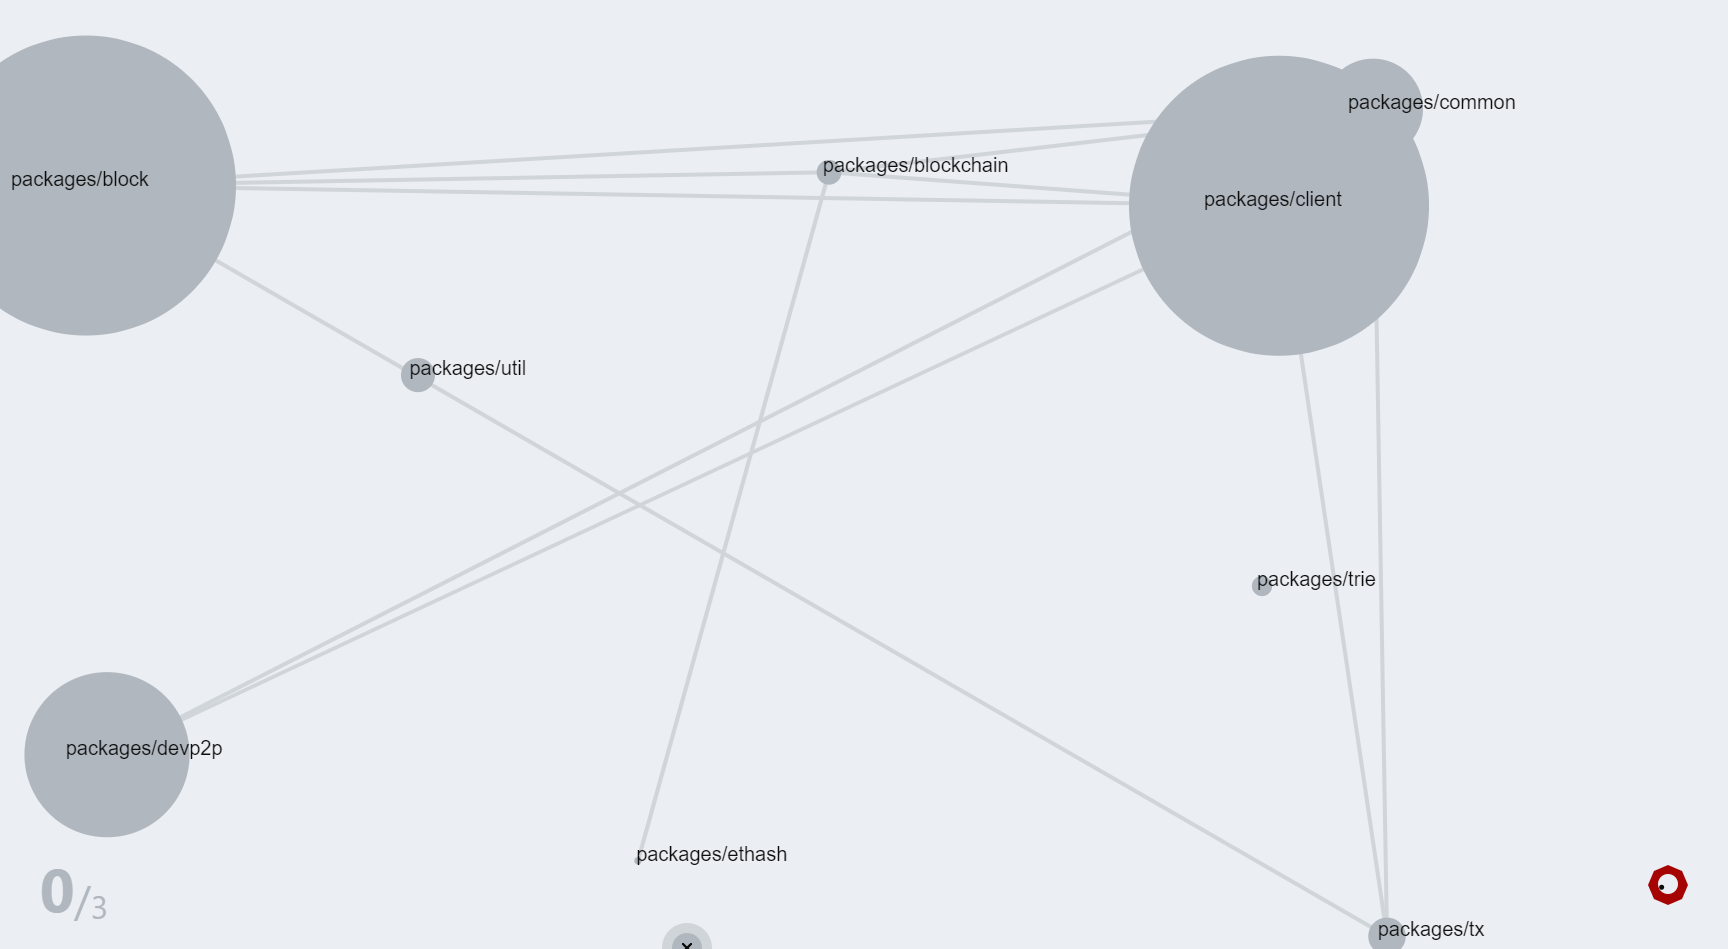
\includegraphics[width=\textwidth]{probesteps/step5.png}

  \subsection*{Step 6: Probe Detail Scene (Example)}

  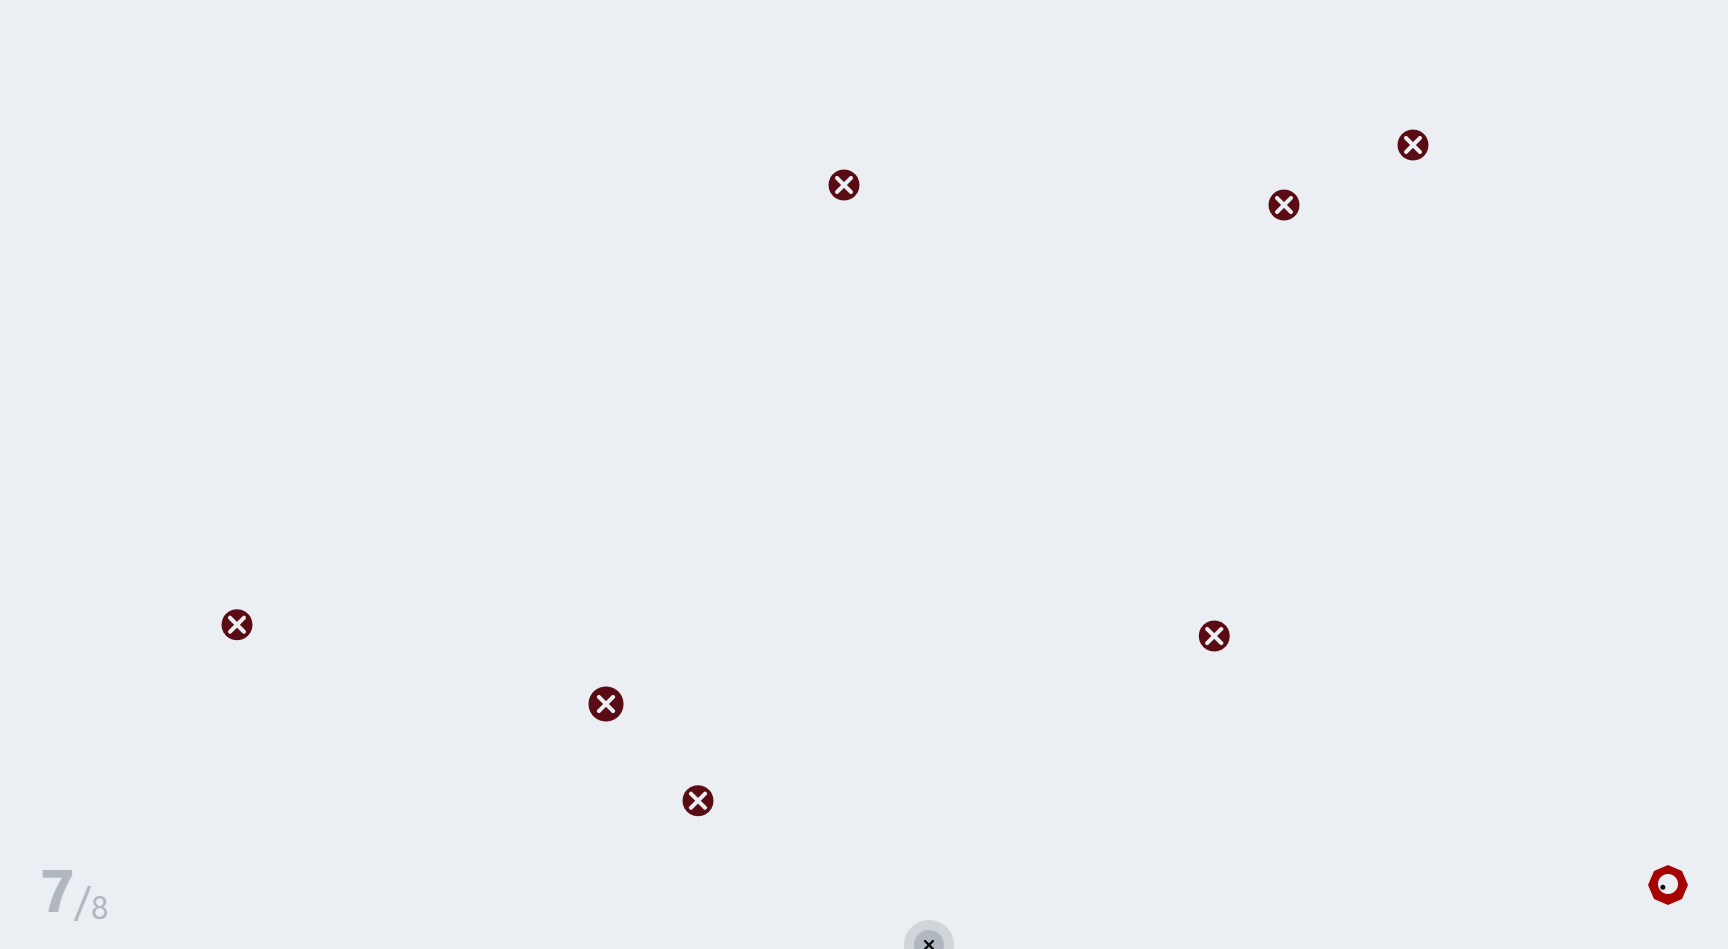
\includegraphics[width=\textwidth]{probesteps/step6.png}

  \subsection*{Step 7: Questions on the underlying project}

  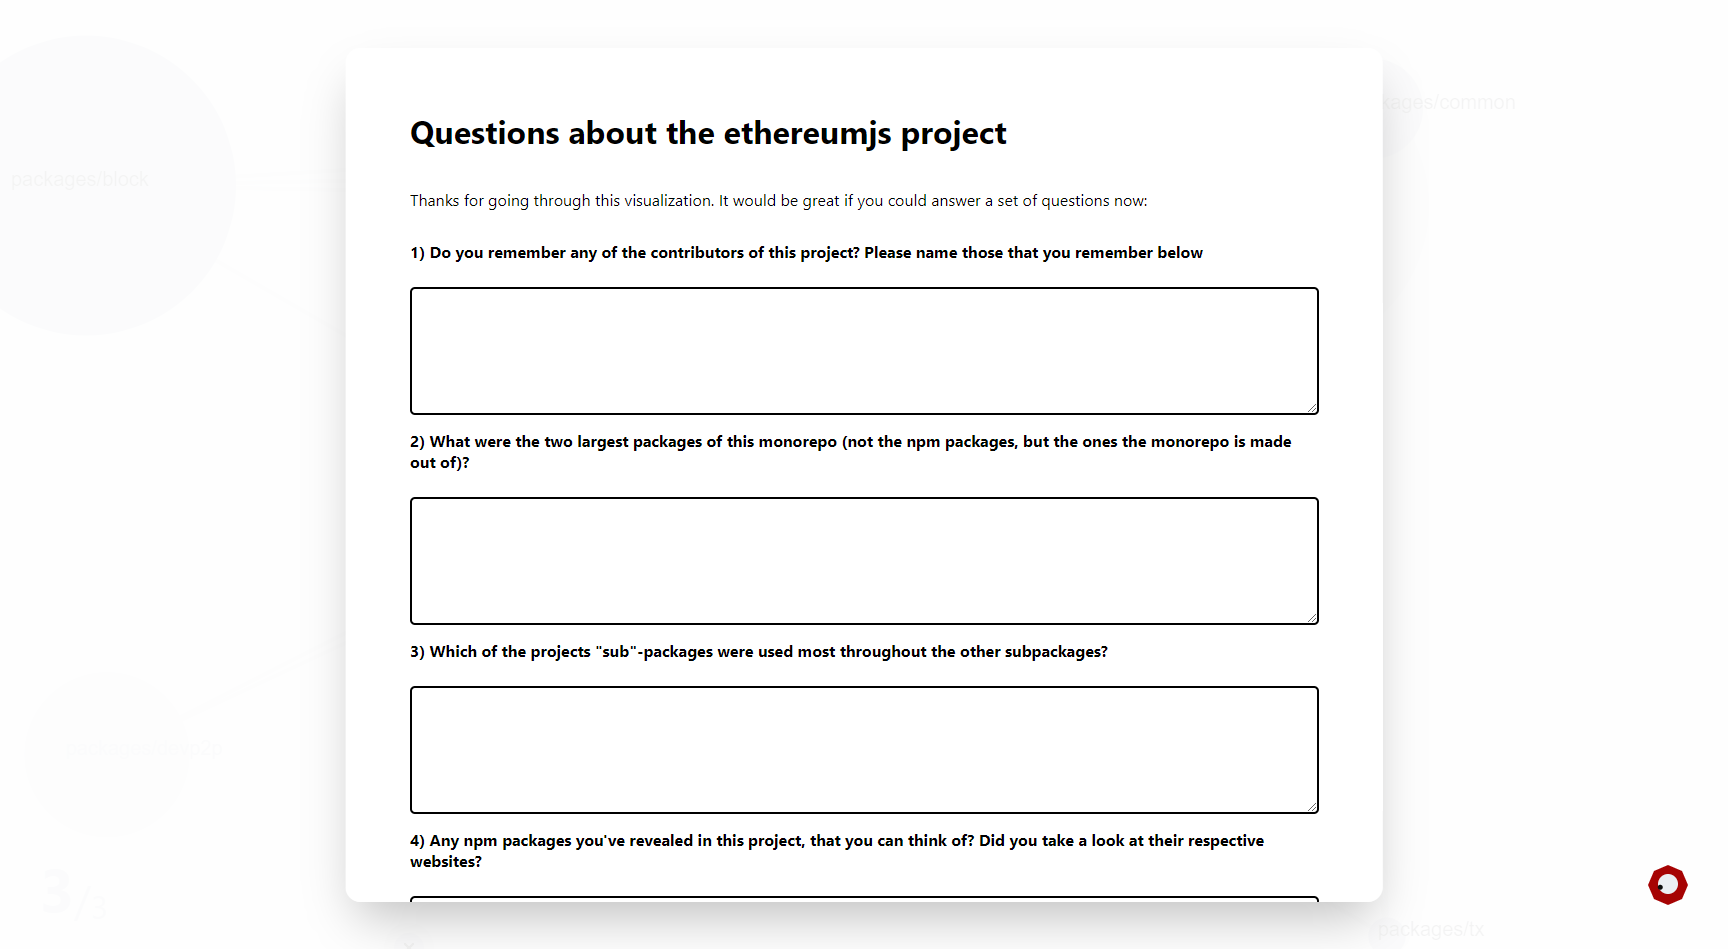
\includegraphics[width=\textwidth]{probesteps/step7.png}

  \subsection*{Step 8: Questions on the research topic}

  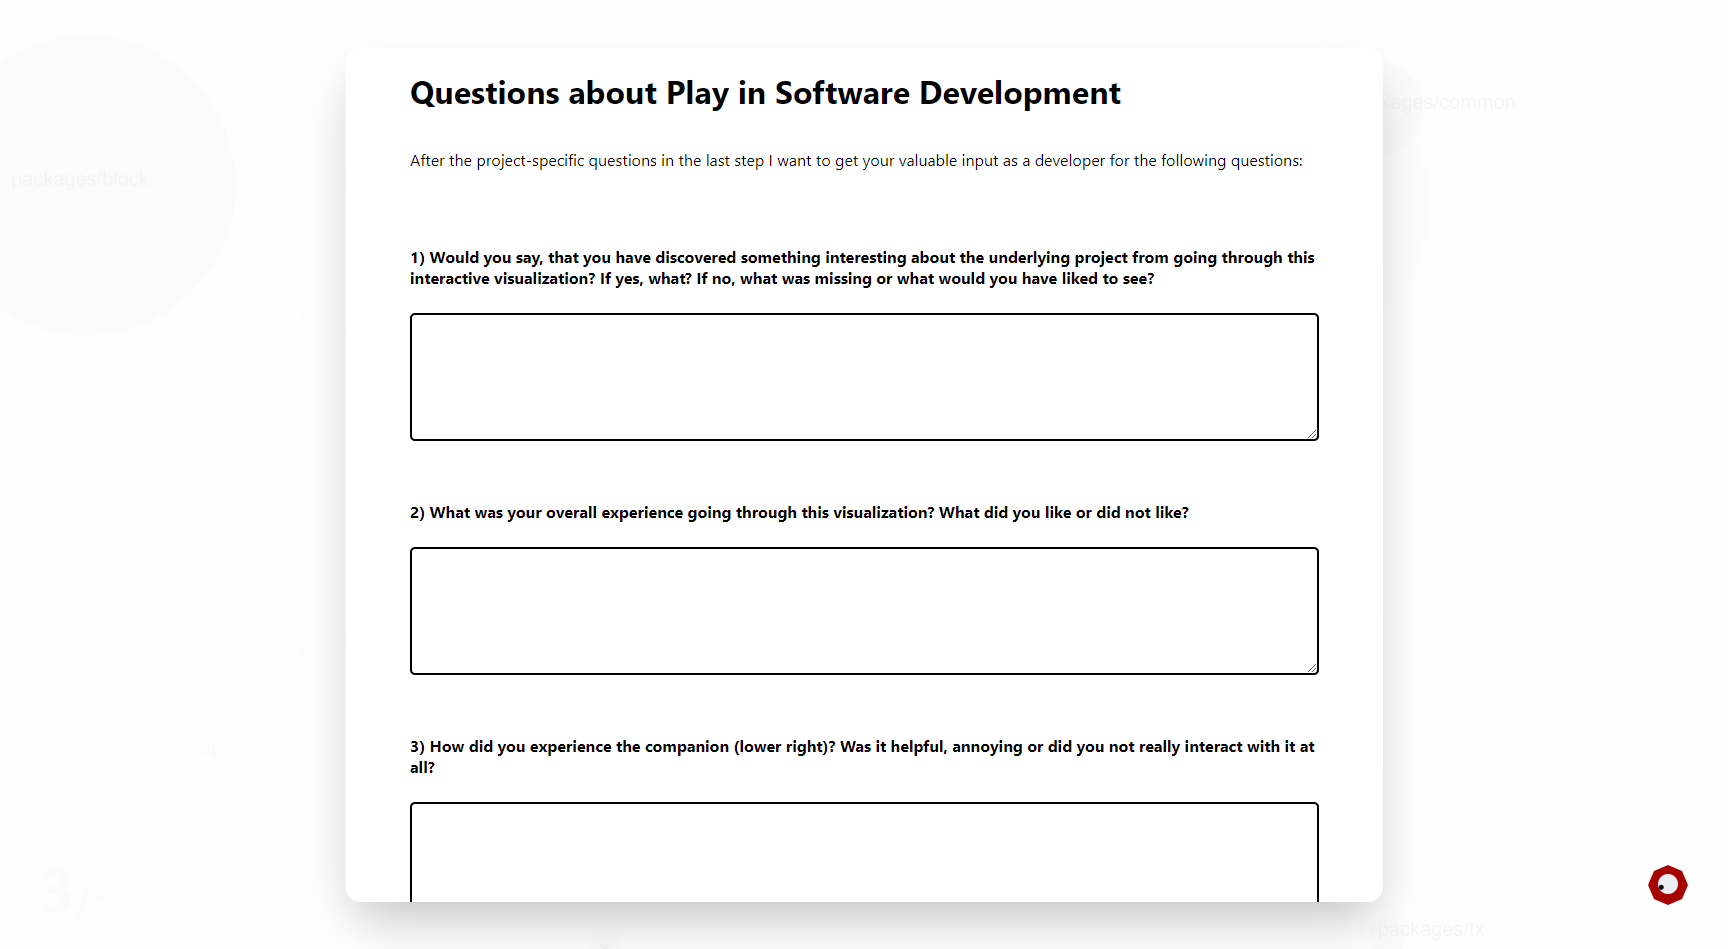
\includegraphics[width=\textwidth]{probesteps/step8.png}

  \subsection*{Step 9: Outro}

  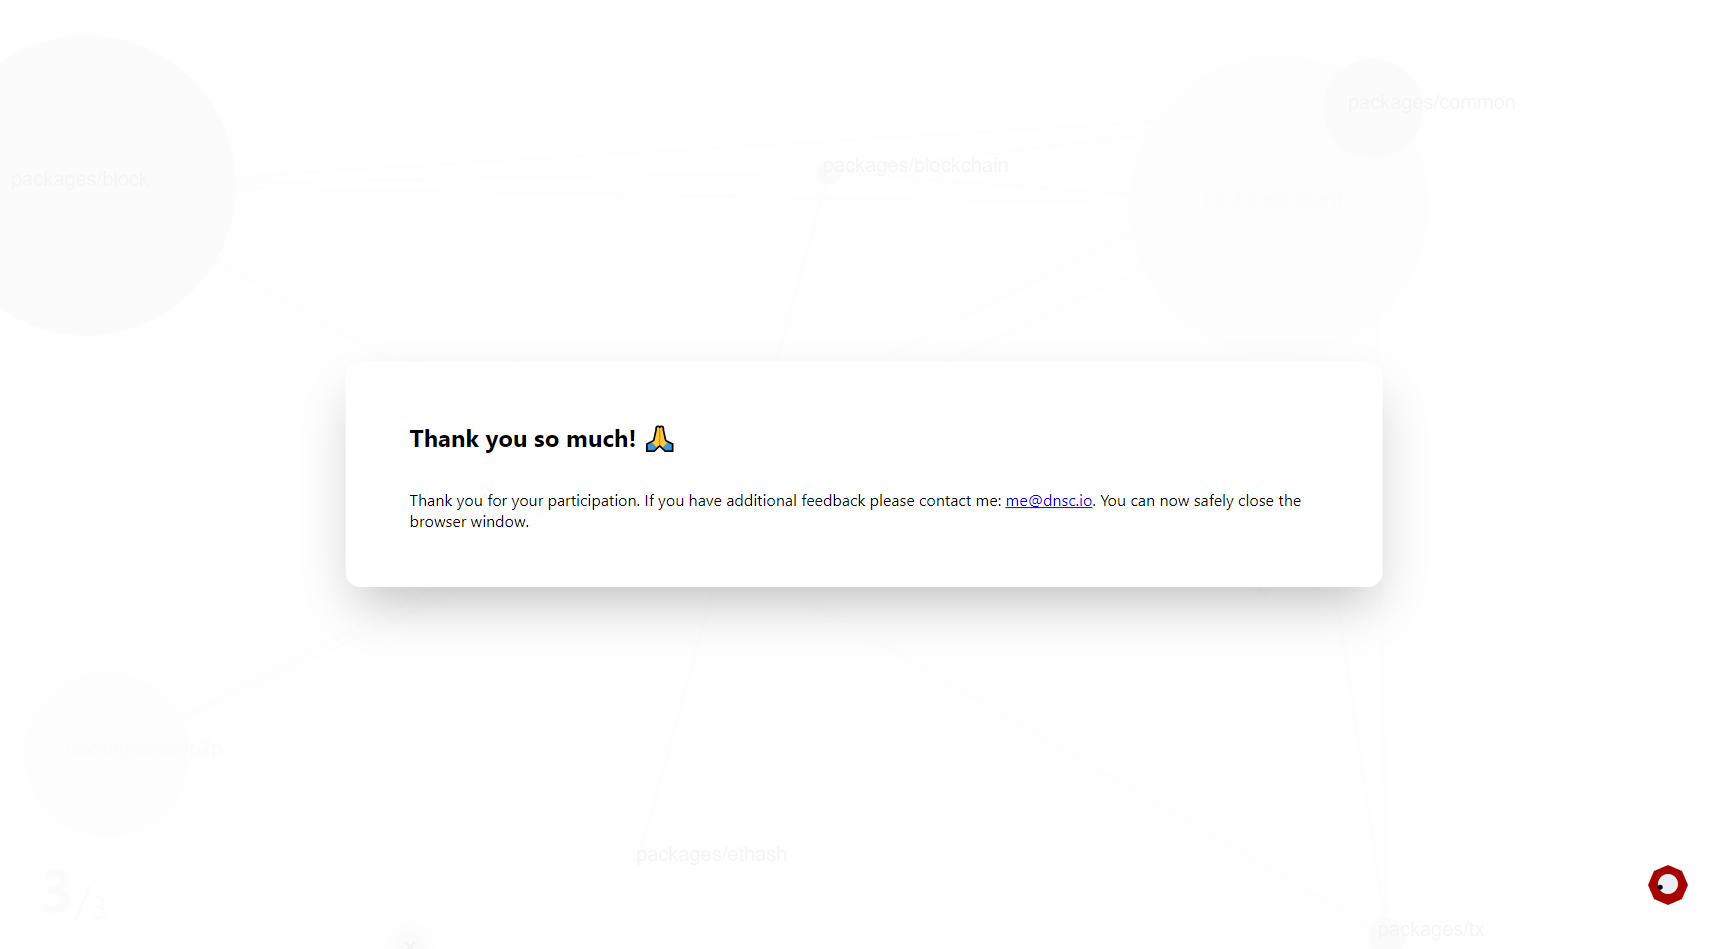
\includegraphics[width=\textwidth]{probesteps/step9.png}

  \newpage
  \section{Participants}
  \label{append:participants}

  \begin{table}[h]
    \begin{tabularx}{\textwidth}{|l|X|l|X|X|}
      \hline
      \textbf{Code} & \textbf{Name} & \textbf{Age} & \textbf{Professional Background} & \textbf{Professional Experience} \\ \hline \hline
      P1            & Anonymous     & 31           & Web Developer                    & 0-1 year                         \\ \hline
      P2            & Anonymous     & 28           & Full Stack Developer             & 1-3 years                        \\ \hline
      P3            & Jens          & 26           & Developer                        & 5-10 years                       \\ \hline
      P4            & Lukas         & 28           & Business Development             & 5-10 years                       \\ \hline
      P5            & Paolo Sfilio  & 28           & Software Developer               & 3-5 years                        \\ \hline
      P6            & Anonymous     & 36           & Backend Developer                & 10+ years                        \\ \hline
      P7            & Anonymous     & 28           & Data Scientist                   & 1-3 years                        \\ \hline
      P8            & Simon Hansen  & 27           & Web Developer                    & 3-5 years                        \\ \hline
      P9            & Anonymous     & 24           & .Net Dev                         & 3-5 years                        \\ \hline
    \end{tabularx}
  \end{table}


  \newpage
  \section{Aggregated Data from the Technology Probe Logs}
  \label{append:log-aggregated}

  Following are the general data points for each participant, aggregated from the raw logs of the technology probe. This text was generated programmatically, the respective script can be found within the accompanying repository at \texttt{./supplementary-material/data-analysis/aggregate-logs/aggregate-logs.js}.

  \subsection*{Participants}

  \subsubsection*{Participant P1}

  This participant spent a total time of \textbf{5 minutes 19 seconds} within the interactive part of the technology probe.

  During that time the participant clicked within the overview and to reveal (in the detail scenes) \textbf{119} times. The participant also tried to click the companion \textbf{8} times.


  \subsubsection*{Participant P2}

  This participant spent a total time of \textbf{6 minutes 49 seconds} within the interactive part of the technology probe.

  During that time the participant clicked within the overview and to reveal (in the detail scenes) \textbf{589} times. The participant also tried to click the companion \textbf{13} times.


  \subsubsection*{Participant P3}

  This participant spent a total time of \textbf{12 minutes 50 seconds} within the interactive part of the technology probe.

  During that time the participant clicked within the overview and to reveal (in the detail scenes) \textbf{224} times. The participant also tried to click the companion \textbf{10} times.


  \subsubsection*{Participant P4}

  This participant spent a total time of \textbf{3 minutes 15 seconds} within the interactive part of the technology probe.

  During that time the participant clicked within the overview and to reveal (in the detail scenes) \textbf{131} times. The participant also tried to click the companion \textbf{7} times.


  \subsubsection*{Participant P5}

  This participant spent a total time of \textbf{null [ed. note: not finished]} within the interactive part of the technology probe.

  During that time the participant clicked within the overview and to reveal (in the detail scenes) \textbf{40} times. The participant also tried to click the companion \textbf{0} times.


  \subsubsection*{Participant P6}

  This participant spent a total time of \textbf{2 minutes 18 seconds} within the interactive part of the technology probe.

  During that time the participant clicked within the overview and to reveal (in the detail scenes) \textbf{131} times. The participant also tried to click the companion \textbf{4} times.


  \subsubsection*{Participant P7}

  This participant spent a total time of \textbf{8 minutes 14 seconds} within the interactive part of the technology probe.

  During that time the participant clicked within the overview and to reveal (in the detail scenes) \textbf{561} times. The participant also tried to click the companion \textbf{45} times.


  \subsubsection*{Participant P8}

  This participant spent a total time of \textbf{9 minutes 50 seconds} within the interactive part of the technology probe.

  During that time the participant clicked within the overview and to reveal (in the detail scenes) \textbf{185} times. The participant also tried to click the companion \textbf{6} times.


  \subsubsection*{Participant P9}

  This participant spent a total time of \textbf{5 minutes 50 seconds} within the interactive part of the technology probe.

  During that time the participant clicked within the overview and to reveal (in the detail scenes) \textbf{184} times. The participant also tried to click the companion \textbf{6} times.



  \newpage
  \section{Qualitative Data -- Coding Units}
  \label{append:coding}

  On the following pages, the documented coding units for the qualitative content analysis can be found. These are the result of a multi-step process as described in chapter 5. The working document that includes every step of the process (Selection, Marking, Categories, Coding) can be accessed at the supplementary repository at the following path:

  \begin{center}
    \texttt{./supplementary-material/data-analysis/qualitative\_analysis.xslx}
  \end{center}

  \begin{landscape}
    \begin{longtable}{|p{0.8cm}|p{7cm}|p{3cm}|p{3cm}|p{5.5cm}|p{0.5cm}|}
      \hline
      \textbf{Part.} & \textbf{Marked Unit}                                                                                                                                                                                                                                                        & \textbf{Category Code}                   & \textbf{Contextual Unit (Feature)} & \textbf{Contextual Unit (Logs)}                                                                                                                    & \textbf{Nr.} \\ \hline
      \endhead
      %
      P1                   & didn't really care when I did this because I wasn't aware this was a thing                                                                                                                                                                                                  & Experience towards (playful) features    & Contributor Revealable             &                                                                                                                                                    & 1            \\ \hline
      P1                   & no emotional attachment to this project                                                                                                                                                                                                                                     & Contextual Considerations                &                                    &                                                                                                                                                    & 2            \\ \hline
      P1                   & Because contributors don't really help me to get started with a project I guess                                                                                                                                                                                             & Social Onboarding                        &                                    &                                                                                                                                                    & 3            \\ \hline
      P1                   & only had some 80 lines and I thought to myself 'well, that's not that big in my opinion'                                                                                                                                                                                    & Experience towards (playful) features    & Potential Issue Revealable         &                                                                                                                                                    & 4            \\ \hline
      P1                   & I didn't really get the impression of the existance of 'sub' packages, whatever they are supposed to be anyway                                                                                                                                                              & Experience towards (playful) features    & Overview Scene (Subpackages)       &                                                                                                                                                    & 5            \\ \hline
      P1                   & only check out npm packages when I actually have to work with them, not randomly only because they are used in a project                                                                                                                                                    & Technical Onboarding                     &                                    &                                                                                                                                                    & 6            \\ \hline
      P1                   & Not exactly sure what you mean with 'legacy' file                                                                                                                                                                                                                           & Experience towards (playful) features    & Potential Issue Revealable         &                                                                                                                                                    & 7            \\ \hline
      P1                   & actually interesting to get told about contributors and see their faces. Not that it would really help me getting into this project but yeah, gives it a more personal flavor                                                                                               & Social Onboarding                        &                                    &                                                                                                                                                    & 8            \\ \hline
      P1                   & during each discovery was still a bit big to digest in a playfull way I think                                                                                                                                                                                               & Attitude towards Playful elements        &                                    &                                                                                                                                                    & 9            \\ \hline
      P1                   & visualizations like images/icons rather than just plain text and a sample of the code and a link to the actual file                                                                                                                                                         & Improvements for implemented features    &                                    &                                                                                                                                                    & 10           \\ \hline
      P1                   & or an icon I learned earlier this represents a contributor                                                                                                                                                                                                                  & Improvements for implemented features    &                                    &                                                                                                                                                    & 11           \\ \hline
      P1                   & The texts where pretty repetitive and I stopped reading after 'contributor' so I might've missed any information that was unique to this slide                                                                                                                              & Experience towards (playful) features    &                                    &                                                                                                                                                    & 12           \\ \hline
      P1                   & I was a bit confused because I didn't know what to do when I reached the first blank slide                                                                                                                                                                                  & Experience towards (playful) features    &                                    & Can also be seen in the logs, No action at all in the beginning,  until companion message in both detail and overview scene (see logs lines 10-63) & 13           \\ \hline
      P1                   & helper on the bottom was quick to assist, though                                                                                                                                                                                                                            & Experience towards (playful) features    &                                    &                                                                                                                                                    & 14           \\ \hline
      P1                   & elements disappear, I would make them fade out rather than just getting invisible instantly                                                                                                                                                                                 & Improvements for implemented features    &                                    &                                                                                                                                                    & 15           \\ \hline
      P1                   & impression of revealing areas better when the initial background would be dark and when you trigger the sonar, everything inside the expanding circle is bright. Maybe with some something visual in the background that gives some depth perception.                       & Improvements for implemented features    &                                    &                                                                                                                                                    & 16           \\ \hline
      P1                   & came to help always at the right time. Good guy!                                                                                                                                                                                                                            & Experience towards (playful) features    &                                    & Both companion helping messages were shown, as seen in the logs (log lines 10, 60)                                                                 & 17           \\ \hline
      P1                   & To be honest, I don't really know. It strongly depends on the urgency to get familiar with a project I guess                                                                                                                                                                & Attitude towards Play in Onboarding      &                                    &                                                                                                                                                    & 18           \\ \hline
      P1                   & Exploring something like in this example can be frustrating if you really just want to get the gist of something because you stumble accross so many random things                                                                                                          & Attitude towards Play in Onboarding      &                                    &                                                                                                                                                    & 19           \\ \hline
      P1                   & this kind of visualization isn't the right thing to learn about a coding project. At least not for me.                                                                                                                                                                      & Attitude towards Play in Onboarding      &                                    &                                                                                                                                                    & 20           \\ \hline
      P1                   & hadn't had too much of these occations yet                                                                                                                                                                                                                                  & Organizational Onboarding                &                                    &                                                                                                                                                    & 21           \\ \hline
      P1                   & I set it up first to get a feeling for what I'm dealing with (if possible) and than I dig deeper into it                                                                                                                                                                    & Technical Onboarding                     &                                    &                                                                                                                                                    & 22           \\ \hline
      P1                   & I talk to those who set up or work on the project if possible                                                                                                                                                                                                               & Social Onboarding                        &                                    &                                                                                                                                                    & 23           \\ \hline
      P1                   & for my IDE, it's mostly stuff that helps visualize things like pairs of brackets and key words or variables vs functions and so on.                                                                                                                                         & Technical Onboarding                     &                                    &                                                                                                                                                    & 24           \\ \hline
      P1                   & I try to stick to conventions and write code that's hopefully easy to understand with meaningful variable and function names                                                                                                                                                & Technical Onboarding                     &                                    &                                                                                                                                                    & 25           \\ \hline
      P1                   & I'd provide some extra goals, like the first 5 questions about contributers I remember or not and so on so the explorer has something to aim for                                                                                                                            & Ideas on Playful Elements for Onboarding &                                    &                                                                                                                                                    & 26           \\ \hline
      P1                   & 'quests' can be aimed to point out core concepts of the project and guide the participant towards them.                                                                                                                                                                     & Ideas on Playful Elements for Onboarding &                                    &                                                                                                                                                    & 27           \\ \hline
      P1                   & Gamification is great to learn things like coding itself, like exploring a story with command line operations                                                                                                                                                               & Ideas on Playful Elements for Onboarding &                                    &                                                                                                                                                    & 28           \\ \hline
      P1                   & Exploring something in a playful way also needs to be done it each person's personal pace                                                                                                                                                                                   & Attitude towards Play in Onboarding      &                                    &                                                                                                                                                    & 29           \\ \hline
      P1                   & exploring something also needs time and is not fun if you are under preasure and you just want to get the gist of something                                                                                                                                                 & Attitude towards Play in Onboarding      &                                    &                                                                                                                                                    & 30           \\ \hline
      P1                   & As you did it in your example, I want to have the headspace to branch out and check out parts of the project that are maybe just nice to know but necessarely helping me with actually working on the project                                                               & Attitude towards Play in Onboarding      &                                    &                                                                                                                                                    & 31           \\ \hline
      P1                   & make the participants make solving problems, like searching for an answer for a specific question                                                                                                                                                                           & Ideas on Playful Elements for Onboarding &                                    &                                                                                                                                                    & 32           \\ \hline
      P1                   & let the participant choose a goal and give him or her some sort of quest line with a bunch of sub goals to achieve                                                                                                                                                          & Ideas on Playful Elements for Onboarding &                                    &                                                                                                                                                    & 33           \\ \hline
      P1                   & letting them to search for reusable components which are used throughout the project to make them aware they exist                                                                                                                                                          & Ideas on Onboarding Elements             &                                    &                                                                                                                                                    & 34           \\ \hline
      P1                   & what dependencies a main component has. Then you have just a portion of npm packages to digest                                                                                                                                                                              & Ideas on Onboarding Elements             &                                    &                                                                                                                                                    & 35           \\ \hline
      P1                   & Serve the project guided and bit by bit, only giving participants the choice what main goal they have or they want to achieve by playing this 'quest line'.                                                                                                                 & Ideas on Playful Elements for Onboarding &                                    &                                                                                                                                                    & 36           \\ \hline
      P3                   & Ich habe mir aber ein paar Profile angeguckt                                                                                                                                                                                                                                & Experience towards (playful) features    & Contributor Revealable             &                                                                                                                                                    & 37           \\ \hline
      P3                   & Anhang der Größe und Zeilenmenge hätte ich dem \textbackslash{}"refactor-worthy\textbackslash{}" aber in den meisten Fällen vermutlich zugestimmt.                                                                                                                          & Experience towards (playful) features    & Potential Issue Revealable         &                                                                                                                                                    & 38           \\ \hline
      P3                   & ungefähre Vorstellung davon bekommen, wie die Projekte untereinander zusammenhängen                                                                                                                                                                                         & Experience towards (playful) features    &                                    &                                                                                                                                                    & 39           \\ \hline
      P3                   & wenn ich es mir nicht merken konnte, war eine Visualisierung auf alle Fälle hilfreich                                                                                                                                                                                       & Experience towards (playful) features    &                                    &                                                                                                                                                    & 40           \\ \hline
      P3                   & schön durch die Vorstellung der Contributors ein paar Namen kennenzulernen, denen man im weiteren Verlauf des Projekt vermutlich häufiger über den Weg laufen wird                                                                                                          & Experience towards (playful) features    & Contributor Revealable             &                                                                                                                                                    & 41           \\ \hline
      P3                   & Mit der Vorstellung der großen \textbackslash{}"refactor-worthy\textbackslash{}" Dateien werden einem direkt mehrere Möglichkeiten eröffnet, in das Projekt einzusteigen                                                                                                    & Experience towards (playful) features    & Potential Issue Revealable         &                                                                                                                                                    & 42           \\ \hline
      P3                   & Mir fehlte ein wenig das fachliche über das Projekt. Was tut es? Wofür ist es gut? Nur anhand des Codes ist das schwierig zu verstehen.                                                                                                                                     & Improvements for implemented features    &                                    &                                                                                                                                                    & 43           \\ \hline
      P3                   & Im ersten Moment wusste ich nicht, wie ich starten sollte                                                                                                                                                                                                                   & Experience towards (playful) features    &                                    & As seen in the logs, companion messages appeared in both scenes (lines 9040, 9090)                                                                 & 44           \\ \hline
      P3                   & urch die Hilfen habe ich aber sehr schnell verstanden, wie der Ablauf gedacht ist                                                                                                                                                                                           & Experience towards (playful) features    &                                    & Both messages seen, after that clicking started as can be seen in logs (9040 and following, 9090 and following)                                    & 45           \\ \hline
      P3                   & Suchen der verschiedenen Punkte hat im ersten Moment Spaß gemacht, wurde anschließend aber ein bisschen nervig (vor allem weil einige Punkte vor einem abgehauen sind).                                                                                                     & Experience towards (playful) features    &                                    &                                                                                                                                                    & 46           \\ \hline
      P3                   & hilfreich um zu verstehen, wie das Onboarding zu bedienen ist                                                                                                                                                                                                               & Experience towards (playful) features    &                                    &                                                                                                                                                    & 47           \\ \hline
      P3                   & Leider sagt er nichts, wenn man auf ihn klick                                                                                                                                                                                                                               & Experience towards (playful) features    &                                    &                                                                                                                                                    & 48           \\ \hline
      P3                   & Wiederholung der Hilfe oder irgendein Feedback wären nett gewesen.                                                                                                                                                                                                          & Improvements for implemented features    &                                    &                                                                                                                                                    & 49           \\ \hline
      P3                   & ganz groben ersten Überblick über das Projekt zu verschaffen, würde ich so eine Visualisierung durchaus gut finden                                                                                                                                                          & Attitude towards Play in Onboarding      &                                    &                                                                                                                                                    & 50           \\ \hline
      P3                   & Wenn ich an einem neuen Projekt anfange, arbeite ich mich von außen immer weiter rein                                                                                                                                                                                       & Technical Onboarding                     &                                    &                                                                                                                                                    & 51           \\ \hline
      P3                   & Ablauf des Codes anhand von konkreten Interaktionen mit dem Programm                                                                                                                                                                                                        & Technical Onboarding                     &                                    &                                                                                                                                                    & 52           \\ \hline
      P3                   & Austausch mit erfahrenen Entwicklern finde ich dabei sehr wichtig                                                                                                                                                                                                           & Social Onboarding                        &                                    &                                                                                                                                                    & 53           \\ \hline
      P3                   & das durchgucken alter Issues und deren Lösungen finde ich immer sehr hilfreich                                                                                                                                                                                              & Organizational Onboarding                &                                    &                                                                                                                                                    & 54           \\ \hline
      P3                   & Entweder mir fällt selber ein Fehler/Verbesserung auf und ich möchte es umsetzen oder ich sehe Issues anderer Benutzer und möchte diese Lösen                                                                                                                               & Organizational Onboarding                &                                    &                                                                                                                                                    & 55           \\ \hline
      P3                   & versuche ich mich von oben nach unten durch den Code zu \textbackslash{}"wühlen\textbackslash{}" um irgendwann an der Stelle anzukommen, an der ich etwas ändern/verbessern möchte                                                                                          & Technical Onboarding                     &                                    &                                                                                                                                                    & 56           \\ \hline
      P3                   & verzweige ich oft in die verschiedenen Bereiche des Codes, die an dieser Stelle verwendet werden. So lerne ich nach und nach die Funktionen kennen und wie sie verwendet werden                                                                                             & Technical Onboarding                     &                                    &                                                                                                                                                    & 57           \\ \hline
      P3                   & Ich fände ein Beispiel-Issue spannend. Ein Fehlverhalten, das einem präsentiert wird und das man zu lösen hat. Das Beispiel-Issue sollte so gewählt sein, dass man an vielen wichtigen Stellen des Codes vorbeikommt                                                        & Ideas on Onboarding Elements             &                                    &                                                                                                                                                    & 58           \\ \hline
      P3                   & bevorzuge doch mehr den direkten Kontakt zu Kollegen/Contributors und das selbständige Entdecken des Codes.                                                                                                                                                                 & Social Onboarding                        &                                    &                                                                                                                                                    & 59           \\ \hline
      P3                   & Für den allerersten Überblick und eventuell einer fachlichen Vorstellung der Software finde ich spielerische Elemente durchaus angebracht                                                                                                                                   & Attitude towards Play in Onboarding      &                                    &                                                                                                                                                    & 60           \\ \hline
      P3                   & mehr bei den Open Source Projekten sehen, weil hier oft eine direkte und nahe Kommunikation mit anderen Entwicklern nur schwer möglich ist                                                                                                                                  & Contextual Considerations                &                                    &                                                                                                                                                    & 61           \\ \hline
      P3                   & Im Arbeitsumfeld sind Kollegen eher greifbar und bei Fragen ansprechbar                                                                                                                                                                                                     & Contextual Considerations                &                                    &                                                                                                                                                    & 62           \\ \hline
      P3                   & Vielleicht mit einem Art Wettbewerb wer einen gewissen Workflow schneller durchgespielt hat                                                                                                                                                                                 & Ideas on Playful Elements for Onboarding &                                    &                                                                                                                                                    & 63           \\ \hline
      P6                   & but many of the connections were overlapping, hard to see                                                                                                                                                                                                                   & Experience towards (playful) features    &                                    &                                                                                                                                                    & 64           \\ \hline
      P6                   & line/file size alone does not tell the whole story                                                                                                                                                                                                                          & Improvements for implemented features    &                                    &                                                                                                                                                    & 65           \\ \hline
      P6                   & Liked the connections and the overview map, helped me see at a glance what is in the project                                                                                                                                                                                & Experience towards (playful) features    &                                    &                                                                                                                                                    & 66           \\ \hline
      P6                   & missed actual textual content of the project besides the previews, maybe include more of the contents of the underyling project                                                                                                                                             & Improvements for implemented features    &                                    &                                                                                                                                                    & 67           \\ \hline
      P6                   & Liked the little worm character, felt smooth                                                                                                                                                                                                                                & Experience towards (playful) features    &                                    &                                                                                                                                                    & 68           \\ \hline
      P6                   & would have liked more connection to the source                                                                                                                                                                                                                              & Improvements for implemented features    &                                    &                                                                                                                                                    & 69           \\ \hline
      P6                   & Helpful as far as indicating what I have done                                                                                                                                                                                                                               & Experience towards (playful) features    & Companion                          &                                                                                                                                                    & 70           \\ \hline
      P6                   & not much interaction with it, could not click it besides messages                                                                                                                                                                                                           & Experience towards (playful) features    & Companion                          &                                                                                                                                                    & 71           \\ \hline
      P6                   & would like to see it on projects of another programming language\textbackslash{}nespecially those that maybe are not as cleanly divided into sub projects                                                                                                                   & Attitude towards Play in Onboarding      &                                    &                                                                                                                                                    & 72           \\ \hline
      P6                   & would have also liked to see more of the structure of the single sub projects                                                                                                                                                                                               & Improvements for implemented features    &                                    &                                                                                                                                                    & 73           \\ \hline
      P6                   & would probably still go at new projects in the IDE itself, seems more efficient at least for the source code                                                                                                                                                                & Attitude towards Play in Onboarding      &                                    &                                                                                                                                                    & 74           \\ \hline
      P6                   & I try to get access to everything that I need (git, deployment server, ...) and then set up the project locally and try to build it                                                                                                                                         & Technical Onboarding                     &                                    &                                                                                                                                                    & 75           \\ \hline
      P6                   & if there is at any point problems I try to contact the person who wrote the code otherwise the other team members already in the project                                                                                                                                    & Social Onboarding                        &                                    &                                                                                                                                                    & 76           \\ \hline
      P6                   & Best case there is documentation for the initial setup, but that is often missing                                                                                                                                                                                           & Organizational Onboarding                &                                    &                                                                                                                                                    & 77           \\ \hline
      P6                   & try to talk to project management to get to know the organizational structure                                                                                                                                                                                               & Organizational Onboarding                &                                    &                                                                                                                                                    & 78           \\ \hline
      P6                   & Navigation in code I do with IntelliJ and go-to-definition most of the time                                                                                                                                                                                                 & Technical Onboarding                     &                                    &                                                                                                                                                    & 79           \\ \hline
      P6                   & first step is always the documentation, if there are problems I google or search through the issue list of the package                                                                                                                                                      & Technical Onboarding                     &                                    &                                                                                                                                                    & 80           \\ \hline
      P6                   & For the source code, would have liked an approach that is near to the code, maybe within the IDE itself and more textual or a little helper within the IDE acting playful                                                                                                   & Improvements for implemented features    &                                    &                                                                                                                                                    & 81           \\ \hline
      P6                   & project organization structure maybe a clearer picture of who to talk to and communication with them as part of a game                                                                                                                                                      & Improvements for implemented features    &                                    &                                                                                                                                                    & 82           \\ \hline
      P6                   & do not think it can be efficient in day-to-day work                                                                                                                                                                                                                         & Attitude towards Play in Onboarding      &                                    &                                                                                                                                                    & 83           \\ \hline
      P6                   & maybe for looking at open source projects out of interests                                                                                                                                                                                                                  & Contextual Considerations                &                                    &                                                                                                                                                    & 84           \\ \hline
      P6                   & maybe for young developers or people starting with development                                                                                                                                                                                                              & Contextual Considerations                &                                    &                                                                                                                                                    & 85           \\ \hline
      P6                   & maybe include more of a progress status                                                                                                                                                                                                                                     & Improvements for implemented features    &                                    &                                                                                                                                                    & 86           \\ \hline
      P6                   & go all the way and create a 3D world from a project that you can go through, although that could be way too far from the project                                                                                                                                            & Ideas on Playful Elements for Onboarding &                                    &                                                                                                                                                    & 87           \\ \hline
      P8                   & Some code examples listed below looked to be refactor-worth. For example commented out console logs or very long config values mapped to string in inline calculations.                                                                                                     & Experience towards (playful) features    & Potential Issue Revealable         &                                                                                                                                                    & 88           \\ \hline
      P8                   & surprised that even a major project like ethereumjs has the same problems like many other projects like commented out code or console logs or very big util.ts files                                                                                                        & Technical Onboarding                     & Potential Issue Revealable         &                                                                                                                                                    & 89           \\ \hline
      P8                   & Some basic information like GitHub stars would be cool at the beginning                                                                                                                                                                                                     & Improvements for implemented features    &                                    &                                                                                                                                                    & 90           \\ \hline
      P8                   & I needed some time and the help box to understand, that I was supposed to click somewhere to reveal the information                                                                                                                                                         & Experience towards (playful) features    &                                    & Also can be seen in the logs, on the overview no help was shown, but then in detail scene it was (line 23471, companion message was closed)        & 91           \\ \hline
      P8                   & I had some problems catching the fast moving dots                                                                                                                                                                                                                           & Experience towards (playful) features    &                                    & Relatively long sequence of reveal clicks without clicking on an lement (e.g. json lines 23613-23755)                                              & 92           \\ \hline
      P8                   & That was fun at first, but at the end it was not that much fun anymore to catch the dots, because it was that easy                                                                                                                                                          & Experience towards (playful) features    &                                    &                                                                                                                                                    & 93           \\ \hline
      P8                   & visualisation of all modules looked a bit chaotic. At first I thought, \textbackslash{}"that should help me get a better overview?!\textbackslash{}"                                                                                                                        & Experience towards (playful) features    &                                    &                                                                                                                                                    & 94           \\ \hline
      P8                   & It came up when I was the first time in a sub module and didn't know what to do. There is was very helpful                                                                                                                                                                  & Experience towards (playful) features    & Companion                          & Can be seen on line 23471 - Companion was shown in submodule                                                                                       & 95           \\ \hline
      P8                   & I don't think that I would prefer such a game/interactive visualisation in contrast to just going throw the filestructure, because the game seemed to be a bit random                                                                                                       & Attitude towards Play in Onboarding      &                                    &                                                                                                                                                    & 96           \\ \hline
      P8                   & I don't know if the modules I checked out are the most important ones or not                                                                                                                                                                                                & Improvements for implemented features    &                                    &                                                                                                                                                    & 97           \\ \hline
      P8                   & usually it's a coworker introducing someone new to the project                                                                                                                                                                                                              & Social Onboarding                        &                                    &                                                                                                                                                    & 98           \\ \hline
      P8                   & I'm checking out a new github project, I just roam around and search for some modules and files whose name seem important to me                                                                                                                                             & Technical Onboarding                     &                                    &                                                                                                                                                    & 99           \\ \hline
      P8                   & I just go through the file structure in GitHub and when I wanna dig deeper I open the project in Intellj                                                                                                                                                                    & Technical Onboarding                     &                                    &                                                                                                                                                    & 100          \\ \hline
      P8                   & There could be some moving dots from module to module, depending on how often the module gets imported into another module                                                                                                                                                  & Improvements for implemented features    &                                    &                                                                                                                                                    & 101          \\ \hline
      P8                   & recognise which module is used a lot and which not that often                                                                                                                                                                                                               & Ideas on Onboarding Elements             &                                    &                                                                                                                                                    & 102          \\ \hline
      P8                   & some activity missing, many games have this discover, fight enemies concept                                                                                                                                                                                                 & Ideas on Playful Elements for Onboarding &                                    &                                                                                                                                                    & 103          \\ \hline
      P8                   & This guide is good for discovering                                                                                                                                                                                                                                          & Experience towards (playful) features    & Detail Scene (Within Subpackage)   &                                                                                                                                                    & 104          \\ \hline
      P8                   & some minigames like fighting the bugs or something similar could make it more interesting to play                                                                                                                                                                           & Ideas on Playful Elements for Onboarding &                                    &                                                                                                                                                    & 105          \\ \hline
      P8                   & some videos of the commit history of the project like                                                                                                                                                                                                                       & Ideas on Playful Elements for Onboarding &                                    &                                                                                                                                                    & 106          \\ \hline
      P8                   & In a work environment you are often applied to that project and there is someone who can introduce you                                                                                                                                                                      & Contextual Considerations                &                                    &                                                                                                                                                    & 107          \\ \hline
      P8                   & In open source project often someone new just joins randomly selfmotivated                                                                                                                                                                                                  & Contextual Considerations                &                                    &                                                                                                                                                    & 108          \\ \hline
      P8                   & playful automatic introduction brings more benefits for open source projects, than for work projects                                                                                                                                                                        & Contextual Considerations                &                                    &                                                                                                                                                    & 109          \\ \hline
      P8                   & find x items of y\textbackslash{}" feature (like the pigeons in gta4)                                                                                                                                                                                                       & Ideas on Playful Elements for Onboarding &                                    &                                                                                                                                                    & 110          \\ \hline
      P8                   & Some speaking character introducing with some basic information                                                                                                                                                                                                             & Ideas on Playful Elements for Onboarding &                                    &                                                                                                                                                    & 111          \\ \hline
      P8                   & Some character to follow, like a rabbit or something that you need to follow from module to module                                                                                                                                                                          & Ideas on Playful Elements for Onboarding &                                    &                                                                                                                                                    & 112          \\ \hline
      P8                   & area constraints, so that you discover a certain area, and after some tasks and knowladge gains you are allowed to discover a broader area                                                                                                                                  & Ideas on Playful Elements for Onboarding &                                    &                                                                                                                                                    & 113          \\ \hline
      P9                   & damit hab ich schon gearbeitet, hab aber nicht auf den link gklickt                                                                                                                                                                                                         & Experience towards (playful) features    & Package Revealable                 & went through pretty fast, not read too much in detail probably                                                                                     & 114          \\ \hline
      P9                   & grundsätzlich find ichs vertretbar, dass man bei über 1000 zeilen etwas refactoren sollte                                                                                                                                                                                   & Technical Onboarding                     & Potential Issue Revealable         &                                                                                                                                                    & 115          \\ \hline
      P9                   & übersicht gut, dass man alle packages auf einem platz sieht                                                                                                                                                                                                                 & Experience towards (playful) features    & Package Revealable                 &                                                                                                                                                    & 116          \\ \hline
      P9                   & mehr info zu den packages gewünscht, zusätzlich zu namen und größe, vielleicht direkt in der übersicht                                                                                                                                                                      & Improvements for implemented features    &                                    &                                                                                                                                                    & 117          \\ \hline
      P9                   & infos je package ganz gut, dass man die direkt die personen sieht mit dem was sie als letztes gemacht haben                                                                                                                                                                 & Experience towards (playful) features    & Package Revealable                 &                                                                                                                                                    & 118          \\ \hline
      P9                   & aufdecken war aber bisschen eintönig, da hätte mir was zusätzliches zu machen gefallen                                                                                                                                                                                      & Improvements for implemented features    &                                    &                                                                                                                                                    & 119          \\ \hline
      P9                   & fand die kleine animation mit dem auge ganz gut, aber viel interaktion gab es nicht                                                                                                                                                                                         & Experience towards (playful) features    & Companion                          &                                                                                                                                                    & 120          \\ \hline
      P9                   & gut bei neuen projekten grade bei größeren, wo es sonst schwierig is einen überblick zu bekommen\textbackslash{}nlinux-kernel würde mir einfallen, also bei großen ganz bekannten projekte, bei denen ich aber nicht unbedingt viel mit der programmiersprache gemacht habe & Contextual Considerations                &                                    &                                                                                                                                                    & 121          \\ \hline
      P9                   & klone mir das projekt als erstes und öffne es dann in meiner ide, da gehe ich dann vom main file ausgehend in die unterfiles, je nachdem was ich machen                                                                                                                     & Technical Onboarding                     &                                    &                                                                                                                                                    & 122          \\ \hline
      P9                   & in einer session zusammen die arbeit am projekt anzufangen um direkt einen ansprechpartner für fragen zu haben                                                                                                                                                              & Social Onboarding                        &                                    &                                                                                                                                                    & 123          \\ \hline
      P9                   & grade als einarbeitung in projekte, wo man schwierig einen überblick bekommen kann                                                                                                                                                                                          & Contextual Considerations                &                                    &                                                                                                                                                    & 124          \\ \hline
      P9                   & vielleicht nicht das schnellste, aber um sich spielerisch eine idee zu verschaffen eine gute idee                                                                                                                                                                           & Attitude towards Play in Onboarding      &                                    &                                                                                                                                                    & 125          \\ \hline
    \end{longtable}
  \end{landscape}
\end{appendices}

\end{document}
